%
% Diplomarbeit von Thomas Biege <TheTom@UnixIsNot4Dummies.ORG>
%
% Dank an Patrick "ThE TeX WiZ" Happel :)
%


% TeX Prolog
\documentclass[12pt]{report}
\usepackage{ngerman}
\usepackage{a4}
\usepackage{graphics}
\usepackage{geometry}
\usepackage{hyperref}
\usepackage{graphicx}
\usepackage{capt-of}
\usepackage[numbib,nottoc,chapter]{tocbibind}
\usepackage[nouppercase]{scrpage2}

%\setheadsepline{0.4pt}  %Kopfliniendicke
%\setfootsepline{0.4pt}  %Fussliniendicke

%\setlength{\headheight}{1.1\baselineskip}

%\renewcommand{\headfont}{\tiny\sffamily\slshape}       %Fontformatierung im Kopf
%\renewcommand{\pnumfont}{\small\rmfamily\normalfont}   %Fontformatierung im Fuss

\makeatletter
\renewcommand{\toc@chapter}[1]{%
	\chapter{#1\prw@mkboth{#1}}%
	\phantomsection%
}
\makeatother

%\usepackage{listings}
%\lstset{language=c}
%\renewcommand{\listfigurename}{\chapter{Abbildungsverzeichnis}}
%\renewcommand{\bibname}{\chapter{Literaturverweise}}
%\fontscheme times
%\makeglossary

\begin{document}

%\pagestyle{headings}
\pagestyle{plain}
%\pagestyle{scrheadings}


% Titelseite
\begin{titlepage}
\begin{center}
\vspace*{3cm}
\LARGE{Modulares System zur Erstellung von flexiblen Intrusion--Detection und --Countermeasure--Umgebungen}\\
%\vspace*{2cm}
%\large{Implementierung eines hostbasierten IDS unter Linux}\\
\vspace*{2.5cm}
\large{An der Fachhochschule Dortmund\\
im Fachbereich Informatik\\
erstellte Diplomarbeit\\
im Studiengang \textit{Allgemeine Informatik [Studienrichtung Multimedia]}\\
zur Erlangung des Grades \textit{Diplom--Informatiker (FH)\/} von} \\
\vspace*{2cm}
Thomas Biege, geboren am 19.05.1977\\
\vspace*{2cm}
Erster Betreuer: Prof. Dr. Swik\\
Zweiter Betreuer: Prof. Dr. Eren\\
\vspace*{1cm}
Dortmund, 17. Dezember 2002\\
\end {center}
\end{titlepage}


% Motivation
\thispagestyle{empty}
\section*{\large Motivation}
Der Antrieb f"ur diese Diplomarbeit bestand zum Einen in der Herausforderung
ein Intrusion--Detection--System (IDS) zu entwickeln, zum Anderen sollte die
schlechte Lage der hostbasierten Intrusion--Detection--Systeme im Open--Source--Bereich
verbessert werden.

Aber nicht nur im Open--Source--Bereich, sondern auch in der Forschung
besteht Handlungsbedarf. Dort werden beispielsweise Analyseverfahren zur Erkennung
von Sicherheitsverst"o"sen entwickelt, die dann aber aufgrund von zu hoher
Entwicklungsarbeit nie ihre Laborumgebung verlassen, um in praxistauglichen
System eingesetzt zu werden.

%\pagebreak

% Zusammenfassung
\thispagestyle{empty}
%\begin{center}
%\section*{Zusammenfassung}
\begin{abstract}
Im Laufe der Diplomarbeit wurden eine Reihe von Programmen entwickelt, von denen
jedes eine spezielle Aufgabe erledigt, um das \textit{Common Intrusion--Detection
Framework\/} nachzubilden. Zu den Aufgaben geh"ort das Protokollieren
von Systemaufrufen, das Weiterleiten von Daten, Datenarchivierung, Analyse der
Daten, Management von Alarmen und zu guter Letzt die Reaktion auf erkannte
Angriffe.

Die Programme kommunizieren haupts"achlich "uber ein TCP/IP--Netzwerk,
oder "uber lokale Interprozesskommunikation.

Wichtige Funktionsteile der Programme wurden in Modulen ausgelagert, die
,"ahnlich wie \textit{Shared Libraries\/} oder \textit{Dynamic Linked Libraries\/},
als bin"are Einheiten zur Laufzeit geladen werden k"onnen.

Das beste Beipiel hierf"ur ist der sog. \textit{BufferDaemon\/}. Seine Aufgabe
besteht lediglich darin, Daten vom Netzwerk zu lesen, zwischenzuspeichern und
nach einer gewissen Zeit zu verarbeiten. Diese drei Arbeitsschritte sind in nahezu
jedem Server--Prozess zu finden. Die Abweichungen bestehen lediglich im Datenformat,
sowie in der Datenverarbeitung. Die kontextbezogenen Aufgaben wurden in Modulen
ausgelagert. Dies erm"oglicht dem \textit{BufferDaemon\/}, indem er die
entsprechenden Module l"adt, jedes beliebige Datenformat (Syslog, SNMP, IDMEF/IAP, usw.)
vom Netz zu lesen und zu verarbeiten (Speicherung in einer Datenbank, Analyse,
Verwaltung vom Alarmen, usw.).

Durch die systematische Aufteilung der verschiedenen Aufgaben eines Intrusion
Detection Systems in eigene Programme und Module, die untereinander
kommunizieren k"onnen, erh"alt man die M"oglichkeit, wie in einem
Baukastensystem, ein Intrusion--Detection--System so zusammenzusetzen, dass es
unterschiedlichsten Anforderungen gerecht werden kann. Man kann alle Komponenten
auf einem Rechner laufen lassen oder jedes Programm so verteilen, dass gr"o"sere
Netzwerke "uberwacht werden k"onnen. Es w"are zudem auch denkbar, dass mehrere
Analyseverfahren in einer Hierarchie zusammengeschaltet werden oder die Aussagen
von verschiedenen Analyseverfahren mit Hilfe einer Korrelationseinheit zu einem
endg"ultigen Ergebnis ausgewertet werden. Die Modularisierung macht es Entwicklern
und Forschern einfach, ihre neu entwickelten Verfahren in ein bestehendes System
einzuf"ugen.
\end{abstract}
%\end{center}

% leere Seite
\clearpage
\thispagestyle{empty}
\mbox {~}
\clearpage


% Inhaltsverzeichniss
%\roman{page}
\setcounter{page}{0}
\setcounter{tocdepth}{4}
\thispagestyle{empty}
\tableofcontents


% TEXT %
%\arabic{page}
\setcounter{page}{0}


%
%% Kapitel
%
%\pagestyle{book}
\chapter{Einf"uhrung}
Es gibt kaum noch Firmen, die nicht ans Internet angeschlossen sind;
inzwischen sind sogar in Deutschland rund 31,8 Millionen Privatpersonen "uber
das Internet zu erreichen. Neben klassischen, kabelbezogenen Verbindungen
finden auch immer mehr Internetverbindungen "uber Satelliten oder Funknetzwerke
in der Praxis Anwendung.

Neben der Anzahl der Internetanschl"usse ist auch die Zahl der Angriffe
drastisch gestiegen. Wenn im Jahr 1998 dem \textsc{Computer Emergency Response
Team} (CERT) \cite{www-cert-stats} noch ca. 3.700 Anzeichen f"ur Sicherheitsverst"o"se
(Incidentsreports) gemeldet wurden, waren es im darauffolgenden Jahr mit 9.800 schon mehr
als doppelt so viele. Die H"aufigkeit der Angriffe steigt weiter an, bereits in den ersten
beiden Quartalen des Jahres 2002 sind "uber 43.000 Incidentsreports beim CERT eingegangen.
Diese Zahlen machen einen explosionsartigen Anstieg der Bedrohung im Internet sehr deutlich.

Zur Zeit gibt es vier generelle Ans"atze, um der steigenden Anzahl von Angriffen Herr
zu werden. Zum einen \textit{Firewalls\/}, die als sehr einfaches Mittel f"ur die Zugangskontrolle
auf Netzwerk-- (Packetfilter) und Applikationsebene (Proxy) eingesetzt werden.
Beim Versandt von Daten "uber nicht vertrauensw"urdige Netzwerke wird die Vertraulichkeit,
Echtheit und Integrit"at mit Hilfe von sog. \textit{Virtual Private Networks\/} (VPN) gesch"utzt.
F"ur die sichere Authentifikation von Benutzern wird bspw. \textit{SecurID} von \textsc{RSA Security}
\cite{www-rsasec} eingesetzt. Dabei generiert ein sog. \textit{SecurID} Token in bestimmten
Zeitintervallen ein Einmal--Passwort, welches zur Anmeldung "uber ein unsicheres Medium
benutzt werden kann.
Wenn alle Abwehrma"snahmen fehlgeschlagen sind, dann k"onnen Einbr"uche immer noch durch
\textit{Intrusion--Detection--Systeme\/} (IDS) entdeckt werden.

Intrusion--Detection ist noch ein junges Gebiet der Sicherheitsindustrie;
jedoch wurden die ersten Intrusion--Detection--Systeme bereits in den sechziger Jahren in
amerikanischen Telefonnetzen und in den Achtzigern vom US Milit"ar zur "Uberwachung von
Datenbanken eingesetzt. Man sieht also, dass die Idee schon lange existierte, als noch
niemand an das Internet, in dem Ausma"s wie wir es heute kennen, gedacht hatte. Ende der
neunziger Jahre erlebten Intrusion--Detection--Systeme ihre Renaissance und wurden
f"ur den kommerziellen Bereich wiederentdeckt.

Da die Erkennung von Angriffen in Computersystemen eine sehr komplexe Angelegenheit
ist, die schon viele Richtungen und Ideen hervorgebracht hat, soll zun"achst ein
"Uberblick "uber bestehende Technologien und Ans"atze gegeben werden. Dieser "Uberblick
soll auch helfen, dass hier entwickelte System, \textsc{M--ICE}, besser einzuordnen und
zu bewerten zu k"onnen.



\section{Anforderungen an ein Intrusion--Detection--System}
Im Jahre 1998 hat das \textsc{Bundesamt f"ur die Sicherheit in der Informationstechnik}
(BSI) von der \textsc{debis IT--Security Services GmbH} eine Studie "uber Intrusion--Detection--Systeme
\cite{paper-anforderungen} anfertigen lassen. Neben ID--Grundlagen und Produkt"ubersichten
wurden in Kapitel 4 und 5 Anforderungen an Intrusion--Detection und Intrusion--Response--Systeme
definiert. Es soll hier nur ein Auszug der Forderungen wiedergegeben werden:
\begin{itemize}
%\item Das System muss einfach zu installieren sein.
%\item Die Wartung des IDS muss einfach und kosteng"unstig sein.
%\item Die Verwaltung des Intrusion--Detection--Systems sollte mit Hilfe einer GUI erleichtert werden.
%\item Das IDS soll eine ausf"uhrliche Online--Hilfe zur Verf"ugung stellen.
%\item Das IDS muss Benutzern verschiedener Erfahrungsstufen die n"otigen
%      Informationen liefern k"onnen. D.h. das IDS muss in der Lage sein einem
%      unerfahrenden Benutzer einen Angriff sehr abstrakt darzustellt. Benutzer
%      mit mehr technischem Wissen k"onnen von dem IDS nach Bedarf mit detailierteren
%      Darstellungen versorgt werden.
\item Der Grund f"ur einen Alarm muss vom IDS angezeigt werden k"onnen.
\item Gro"se Datenmengen m"ussen so darstellbar sein, dass eine manuelle
      Verarbeitung m"oglich ist.
%\item Technischer Support sollte vom Hersteller geleistet werden.
\item Angriffssignaturen sollten von dem Hersteller schnell bereitgestellt werden.
\item Eigene Angriffsmuster m"ussen vom Benutzer manuell eingegeben werden k"onnen.
%\item Die Herstellerfirma sollte Trainingskurse f"ur das Personal des Kunden
%      anbieten.
\item Das System, auf dem die IDS--Software l"auft, muss gut abgesichert sein.
\item Das IDS selbst muss gegen Angriffe geh"artet worden sein.
\item Das Produkt muss leicht skalierbar sein.
\item Um effizienter zu arbeiten, sollte das IDS externe, sicherheitsrelevante
      Informationen aufnehmen k"onnen. Beispiel: Urlaubs--, Feier-- und Krankheitstage
\item Das Intrusion--Detection--System sollte hybrid sein, d.h., es sollte Misuse-- und Anomaly Detection
      unterst"utzen.
\item Daten aus mehreren Quellen (Netzwerk, Logfiles, etc.) sollten verarbeitet
      werden k"onnen.
\item Die Daten sollten in \glqq Echtzeit\grqq\/ analysiert werden.
\item Die Authentizit"at der gesammelten Audit--Daten muss gew"ahrleistet werden
      k"onnen.
\item Aus rechtlichen Gr"unden m"ussen Benutzerdaten pseudonymisiert werden.
\item Die unter den einzelnen IDS--Komponenten ausgetauschten Daten m"ussen
      verschl"usselt werden.
\item Die Integrit"at der gesammelten Audit--Daten muss erhalten bleiben. Dies kann
      durch Speicherung auf einmal beschreibare Medien oder durch Kryptographie
      erziehlt werden.
\item Es muss m"oglich sein, die Granularit"at der Audit--Daten zu ver"andern.
      Beispielsweise kann w"ahrend eines Angriffes die Granularit"at erh"oht werden.
\item Mehrere Angriffe m"ussen vom IDS erkannt und priorisiert werden.
\item Beim Ausfall von Komponenten des Intrusion--Detection--Systems muss sofort
      Alarm gegeben werden.
\end{itemize}


\section{Intrusion--Detection--Systemkomponenten}

F"ur unsere Betrachtung soll die IDS--Spezifikation des \textit{Common Intrusion--Detection
Frameworks\/} (CIDF) \cite{www-cidf} verwendet werden. Nach dem CIDF besteht ein IDS aus
vier Komponenten, sog. Boxen.

\begin{itemize}
\item Event (E--) Box
\item Analysis (A--) Box
\item Countermeasure (C--) Box
\item Storage/Data (D--) Box
\end{itemize}

\vspace{1cm}
\begin{center}
	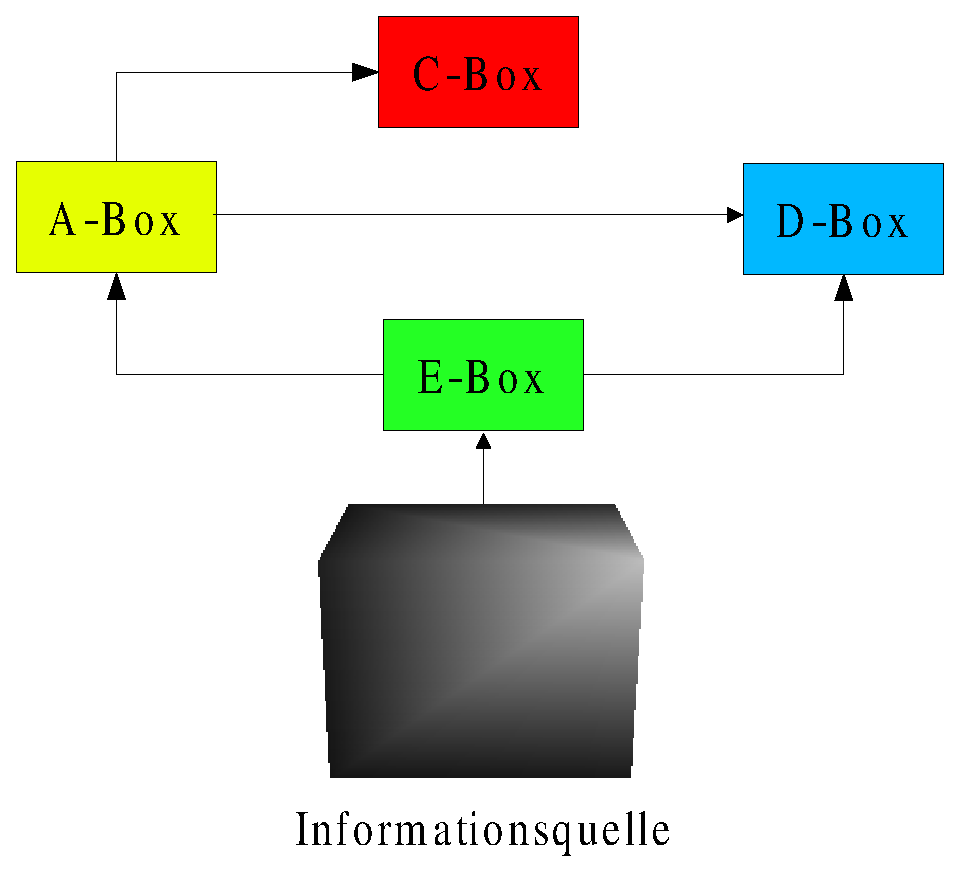
\includegraphics[scale=0.7]{CIDF-Boxen-richtige-groesse.eps}
	\captionof{figure}{CIDF Modell mit E--, D--, A-- und C--Box}
\end{center}
\vspace{1cm}

Die Event--Box ist daf"ur verantwortlich, dass Audit--Daten, in Form von rohen Netzwerkpaketen und/oder
Betriebssystem--Log--Daten aus der Kernel-- und Applikationsebene nahtlos gesammelt werden.
Anschlie"send werden die Daten in ein einheitliches Format (vgl. \cite{draft-idmef}
\cite{paper-bishop} \cite{paper-cisl}) gebracht, an die Analysis--Box versandt und je nach
Konfiguration auch an die Data--Box "ubertragen.
Zuvor sollten jedoch redundante und unwichtige Informationen entfernt werden, um Speicherplatz
zu sparen und die Informationsverarbeitung zu beschleunigen.
In der Analysis--Box findet die Hauptarbeit des IDS statt. Hier werden
die Daten von der Event--Box auf Angriffsmuster, Anomalien und
nicht eingehaltene Sicherheitsvorgaben "uberpr"uft. Existiert f"ur das
gewonnene Analyseresultat eine vom Benutzer definierte Aktion, wird diese
durch die Countermeasure--Box ausgef"uhrt. Desweiteren wir das Analyseergebnis an die Data--Box
weitergeleitet. Folgende Analyseverfahren werden i.d.R. benutzt:

\begin{itemize}
\item Misuse Detection:
	\begin{itemize}
	\item Experten System
	\item Zustandsautomaten (State Transition)
	\item Beschreibungssprachen
	\end{itemize}
\item Anomaly Detection:
	\begin{itemize}
	\item quantitative Analyse
	\item statistische Messungen
	\item regelbasierte Systeme
	\item neuronale Netzwerke
	\end{itemize}
\end{itemize}

Die von der Countermeasure--Box durchgef"uhrten Reaktionen k"onnen zwar
in den verschiedensten Formen auftreten; unterliegen aber grunds"atzlich
zwei Kategorien:

\begin{itemize}
\item Passiv:
	\begin{itemize}
	\item Email verschicken
	\item Nachricht an einen Pager oder Handy senden
	\item Audiodaten abspielen
	\item Dialogfenster "offnen
	%\item Email an den Administrator des attackierenden Systems schicken
	\item etc.
	\end{itemize}

\item Aktiv:
	\begin{itemize}
	\item Menge der aufzuzeichnenden Audit--Daten erh"ohen
	\item kritische oder angegriffene Systeme und Dienste abschalten
	\item Packetfilterregeln von Firewalls anpassen
	\item Informationen "uber das System sammeln, von dem die Angriffe ausgehen
	\item das attackierende Computersystem mit Denial--of--Service (DoS) Attacken ausser Gefecht setzen
	\item etc.
	\end{itemize}
\end{itemize}

Die aktiven Reaktionen werden i.d.R. gar nicht oder sehr selten angewandt, da der Angegriffene,
das Opfer, selbst zum T"ater von Straftaten werden kann. Erschwerend
kommt noch hinzu, dass sich der Angreifer gar nicht auf dem System befinden
muss, von dem die Attacken ausgehen. Der Angreifer kann mit Hilfe von
\textit{IP--Address--Spoofing} \footnote{hierbei wir die Absenderadresse eines IP--Paketes
gef"alscht} seinen wahren Standort verschleiern. Oder das System wird vom Angreifer
nur als Ausgangspunkt seines Angriffs missbraucht. Desweiteren kann der Angreifer
seine Attacken so aussehenen lassen, als w"urden sie von den IP--Adressen
eines Gesch"aftspartnerns kommen. Die C--Box w"urde daraufhin die Firewallkonfiguration
ver"andern, um die Pakete aus dem Partnernetz zu blocken, das h"atte zur Folge, dass eine
Zusammenarbeit nicht mehr m"oglich w"are.

Leider k"onnen die passiven Handlungen der C--Box ebenfalls von dem
Angreifer gegen das zu sch"utzende Netz gewandt werden. Zum Beispiel k"onnen durch
zuviele vom IDS verschickte Alarmmeldungen an Email oder Pager die Mail-
oder Modemserver "uberlasten (Denial--of--Service Attacke) oder der Security Officer
wird dazu gebracht, die wirklich wichtigen Meldungen zu "ubersehen oder einen
Pager gleich ganz abzuschalten bzw. die Emails ungesehen zu l"oschen.

Um diesen Gefahren entgegenzuwirken kann das IDS bspw. so konfiguriert
werden, dass bestimmte IP--Adressen nicht gesperrt werden, sondern nur
der SO alarmiert oder mit ihm R"ucksprache gehalten wird. Alarmmeldungen desselben Types
in einer bestimmten Zeitspanne sollten nur einmal mit Angabe der Menge an
den SO gemeldet werden.


\section{Intrusion--Detection--Technologien}

\subsection{Audit--Datenquelle und Architekturen}

%Intrusion--Detection--Systeme ziehen verschiedene Datenquellen heran, um ihre
%Analyse durchzuf"uhren.

So vielf"altig, wie die Einsatzgebiete der Intrusion--Detection--Systeme sind, so vielf"altig
sind auch deren Architekturen. Hier sollen nur die verbreiteten Varianten angesprochen werden.
Als erstes m"ussen einige Unklarheiten bei den Begriffen \glqq hostbasiertes\grqq\/ und
\glqq netzbasiertes\grqq\/ IDS aus dem Weg ger"aumt werden.
Der Begriff \glqq hostbasiert\grqq\/ mag suggerieren, dass ein IDS zur "Uberwachung der
Sicherheit von Computersystemen verwendet wird; das ist aber nicht ganz korrekt.
Als hostbasierte Intrusion--Detection--Systeme werden Produkte bezeichnet, die ihre Audit--Daten, also
Kernel-- und Applikations--Log--Daten, von einem Host bekommen. Hostbasierte Intrusion--Detection--Systeme
sind in der Lage 1 bis n Rechner zu "uberwachen, sie sind also nicht auf einen Rechner beschr"ankt.

Netzbasierte Intrusion--Detection--Systeme analysieren Netzwerkdaten, es ist egal wie sie diese
erhalten und wo sie sie sammeln.
Dabei "uberwachen sie die Sicherheit von Computersystem in einem Netzwerk.
H"aufig wird der Fehler gemacht, nur solche Intrusion--Detection--Systeme als netzbasierend zu
bezeichnen, die ihre Daten von einem Netzwerkinterface erhalten, welches im sog.
\textit{Promiscuous--Mode\/} arbeitet, um alle vorbeikommenden Netzpakete mitzulesen.
Solche Systeme sind die klassischen, sensorbasierten Intrusion--Detection--Systeme, neuere Ans"atze
verwenden Agenten (s. AID \cite{www-aid}), die auf den zu "uberwachenden Computersystem
installiert sind, um die Netzpakete aus den unterschiedlichen Schichten des TCP/IP--Stacks
abzufangen und an eine zentrale Analyseeinheit zu schicken.

\subsubsection{Hostbasierte Systeme}
Die hostbasierten Intrusion--Detection--Systeme existieren am L"angsten. Sie wurden vom
amerikanischen Milit"ar eingesetzt, um Datenbank--Hosts o."a. zu "uberwachen.
Im Normalfall werden User--Level Log--Daten (syslog bei Unix Systemen)
und/oder Kernel--Level Log--Daten (z.B. BSM Auditing Subsystem von Solaris,
AIX Audit Subsystem, NT Event Log, Linux Trace Toolkit, Syscalltracker, SCSLog o."a.)
auf Einbruchsmuster untersucht.
Andere H--Intrusion--Detection--Systeme, wie z.B. \textit{PortSentry} \cite{www-psionic}, lauschen auch an
TCP-/UDP-Ports und alarmieren den SO, wenn eine Verbindung zu den
entsprechenden Ports aufgebaut wird.

H--Intrusion--Detection--Systeme haben den Vorteil, dass sie weniger \textit{False Positives} ausl"osen als
netzbasierte Intrusion--Detection--Systeme, da sie genau \glqq wissen\grqq, wie das Computersystem
reagiert. Zudem k"onnen sie auch Angriffe sehen, f"ur die ein N--IDS blind ist,
z.B. Angriffe "uber die Konsole, Modems, verschl"usselte Verbindungen oder
b"osartige Programme (wie \textit{Trojanische Pferde\/} o."a.).

Nachteilig macht sich bemerkbar, dass ein H--IDS auf jedem zu "uberwachenden
Rechner installiert und gewartet werden muss. Denial--of--Service Angriffe,
die Fehler im TCP/IP--Stack eines Systems ausnutzen, k"onnen von einem H--IDS
nicht ausreichend oder sogar gar nicht erkannt werden, weil das System vorher
abst"urtzt und ein hostbasiertes Intrusion--Detection--System i.d.R. auf einer h"oheren Ebene
operiert als ein netzbasiertes IDS.

\subsubsection{Netzbasierte Systeme}
Sensorbasierte N--Intrusion--Detection--Systeme erfreuen sich seit einigen Jahren gro"ser
Beliebtheit, da diese Systeme sich gut zentral verwalten und an zentralen
Punkten einsetzen lassen. Somit kann ein IDS ganze Computernetzwerke einfach mit
Hilfe eines Rechners "uberwachen und es muss nicht an jeden einzelnen Host Hand
angelegt werden.

Diese Eigenschaft macht sensorbasierte N--Intrusion--Detection--Systeme sehr attraktiv, da sie
weniger administrativen und finanziellen Aufwand erfordern.
Die Event--Box eines sensorbasierten N--IDS liest alle Daten, die "uber einen
Netzwerksegment transportiert werden, und reicht sie anschlie"send an die
Analysebox weiter.

Anhand der Informationen in den  \textit{Packet Headern\/} (Flags, Attribute, etc.)
k"onnen DoS--Attacken oder \textit{Scans\/} (Abtasten des Netzwerks auf Rechner oder
Abtasten von Rechnern auf angebotene Dienste) erkannt werden. Die Payload enth"alt
die Daten, die von dem TCP/IP--Stack an die Applikationebene weitergereicht
werden. Diese Daten werden von der A--Box auf Angriffsmuster gepr"uft.
Bei der Verwendung von N--Intrusion--Detection--Systemen treten massive Probleme auf, die
teilweise in der Zukunft noch gr"o"sere Auswirkungen haben werden.

Das offensichtlichste Problem, dem sensorbasierte N--Intrusion--Detection--Systeme
gegen"uberstehen, ist die Verschl"usselung der Daten. Nicht nur VPN--L"osungen wie \textit{IPsec\/} o."a.,
sondern auch chiffrierte Login--Verbindungen, wie bei
\textit{Secure Shell\/} (SSH), machen ein klassisches N--IDS blind. Die Daten k"onnen nicht dechiffriert
und somit auch nicht analysiert werden. In solchen F"allen ist ein hostbasiertes
System klar im Vorteil. Der Versuch, diesem Problem mit einer \textit{Public Key
Infrastructure\/} (PKI) oder "ahnlichen Keymanagementverfahren begegnen zu wollen,
ist nicht sinnvoll, da dadurch die Komplexit"at stark erh"oht w"urde, und somit
die Robustheit des IDS sinkt. Zudem w"urde sich die Analyse extrem
verlangsamen, da kryptografische Algorithmen, vor allem asymmetrische,
rechenintensiv sind. Weiterhin kommt erschwerend hinzu, dass nicht alle Protokolle
und Dienste mit einer PKI zusammenarbeiten k"onnen.

Die wachsende Netzwerkbandbreite macht es einem sensorbasierten
N--IDS schwer, alle Daten nahtlos zu lesen, ohne dass interne (Ring-) Puffer
"uberlaufen und Daten verloren gehen. Der \textit{Network Flight Recorder\/} bspw. schafft
es, ein saturiertes 100MBit Netzwerk zu "uberwachen. Jedoch existieren inzwischen
Technologien im Gigabitbereich, die auch f"ur den NFR ein Problem darstellen k"onnten.

Ein weitere H"urde, die es zu bew"altigen gilt, stellt die geswitchte
Netzwerkinfrastruktur dar. Im herk"ommlichen \textit{Ethernet} teilen sich alle
Rechner das "Ubertragungsmedium (physikalisches Segment). Das bedeutet,
wenn zwei Rechner gleichzeitig Pakete "ubermitteln
wollen, dann kollidieren die Pakete u. U. und m"ussen erneut versandt
werden. Die Rechner befinden sich also in einer gemeinsamen \textit{Collision Domain}.
Ein Switch vermeidet Kollisionen, indem er jedem Rechner einen
eigenen physikalischen Netzwerkstrang "uber Ports zuweist und die
Pakete genau zu dem Rechner schickt, an den sie adressiert sind. Ein Switch
erzeugt also kleinere physikalische Segmente, in denen sich nur zwei Rechner
befinden, "ahnlich einer Telefonvermittlung. Wenn aber die Netzpakete nur an den
daf"ur vorgesehenden Rechner gelangen, dann kann die E-Box des N--IDS die
Pakte nicht mehr mitlesen; das IDS ist somit wieder einmal blind.

Viele Switches haben einen sog. \textit{Trunk Port\/}, der es dem N--IDS erlaubt, die
Pakete zu lesen. F"ur ein 100MBit Netzwerk hat jeder Port, inkl. \textit{Trunk Port\/},
des Switches eine Bandbreite von 100MBit. Wenn der Switch zehn Ports, ohne \textit{Trunk Port\/},
hat, m"usste der \textit{Trunk Port\/} 10 x 100MBit Bandbreite haben, um alle Daten von allen Ports
mit voller Geschwindigkeit transportieren zu k"onnen; er hat aber nur $\frac{1}{10}$
dieser Bandbreite. Bei schlechter Implementierung der Software auf dem Switch kann bei einem voll
ausgelasteten Netzwerk ein N--IDS u.U. nicht alle Daten lesen. Der \textit{Trunk Port\/} ist also
eher eine Notl"osung f"ur den Intrusion--Detection--Bereich.

Um die Daten analysieren zu k"onnen, muss das sensorbasierte N--IDS
alle g"angigen Netzprotokolle wie IPv4, IPv6, T/TCP, IPX, Appletalk etc. verstehen.
Wenn in dem zu sch"utzenden Netz ein sehr exotischen Protokoll gesprochen wird,
welches der IDS Hersteller nicht implementiert hat, dann ist das IDS somit wertlos.

Die Spezifikationen f"ur den TCP/IP--Stack sind zwar in den \textit{Request for Comments}
(RFC--791 und RFC--793 \cite{www-rfcdb})
Dokumenten vorgegeben, werden aber von jedem Betriebssystemhersteller anders oder unvollst"andig
implementiert. Das hat zur Folge, dass das sensorbasierte N--IDS nie
genau weiss, in welchem Zustand sich der TCP/IP--Stack eines Hosts befindet.
Die Diskrepanz in den verschiedenen Stack--Implementierungen kann sich ein
Angreifer zunutze machen, um seine Pakete gegen"uber dem IDS zu
\glqq verstecken\grqq\/, oder er kann Pakete im Datenstrom des IDS einf"ugen, die das
Zielsystem nicht anerkennt und ignoriert \cite{paper-evasion}.
Dieser Sachverhalt soll an einem einfachen Beispiel erkl"art werden:
Ein Angreifer schickt ein TCP-Paket, welches die Angriffsdaten enth"alt, an einen
unsicheren Netzdienst des Zielsystems.
Die Pr"ufsumme im TCP--Header ist absichtlich falsch berechnet. Das
IDS sieht das Paket, ignoriert es aber, weil die Pr"ufsumme falsch
ist. Das Zielsystem empf"angt das Paket, "uberpr"uft die Pr"ufsumme aber
nicht, weil es nicht implementiert wurde und reicht die Nutzdaten
an die Serverapplikation weiter. Resultat: Das IDS hat das Paket verworfen, aber
das Zielsystem akzeptierte es und der Angreifer konnte das Sicherheitsloch
unbemerkt ausnutzen.

Diese gravierenden Probleme machen den Einsatz von rein sensorbasierten N--Intrusion--Detection--Systemen
bereits heute fraglich.

Knotenbasierte (nodebased) N--Intrusion--Detection--Systeme vermeiden viele Probleme
der klassischen N--Intrusion--Detection--Systeme (s. AID \cite{www-aid}), sind aber aufgrund ihres dezentralen
Charakters nicht so einfach einzusetzen wie ihre Vorg"anger.
Auf den einzelnen Computersystemen werden kleine \glqq Monitore\grqq\/ eingesetzt,
die in den TCP/IP--Stack eingebunden werden, um die Netzwerkpakete auf
einer h"oheren Ebene zu lesen und sie dann zentral (oder auch dezentral) zu
analysieren. Inkonsistenzen bei der Interpretation von Netzverbindungen,
"uberf"ullte Puffer und Verschl"usselungen auf niedrigerer Ebene (\textit{IPsec\/} etc.)
sind somit kein Problem mehr. Verschl"usselung auf h"oherem Level z. B. durch
SSH, PGP, SSL usw. k"onnen aber immer noch nicht im Klartext
betrachtet werden, ausser nat"urlich mit komplizierten Keymanagementverfahren.

\subsubsection{Alternativen}

Neben den host-- und netzbasierten Ans"atzen gibt es noch andere
Entwicklungen in der Architektur von Intrusion--Detection--Systemen, die zum
gro"sen Teil aber keinen gr"o"seren Einsatz in der Praxis fanden (z. B. mobile autonomous
Agents). Die bekannteste Form ist wohl der \textit{Honeypot\/}, der dem Angreifer ein
verwundbares System vorgaukelt.

\paragraph*{Honeypot Systeme}
Honeypots sind Systeme, die vorgeben, Sicherheitsl"ucken zu haben.
Wenn ein Angreifer dieses System entdeckt, dann wird er es
attackieren und keine Probleme haben, die Sicherheitsmechanismen zu
"uberwinden. Der Angreifer denkt, er befindet sich auf einem normalen
Computersystem, wurde in Wahrheit aber in eine
abgeschottete Umgebung umgeleitet. Der SO wird dar"uber
benachrichtigt und hat nun die M"oglichkeit, das Verhalten des Angreifers
zu beoabachten und zu analysieren. Somit ist es vielleicht m"oglich, das
Bestreben des Angreifers zu erkennen oder sogar neue Angriffsformen zu
entdecken.
\textit{Das Deception Toolkit\/} (DTK) und \textit{ManTrap\/} sind gute Beispiele f"ur ein
hostbasiertes Honeypot System.
Theoretisch sind auch netzbasierte Honeypots (Honeynet) m"oglich, die
dem Angreifer ein ganzes Netz vorgaukeln, indem sie auf einem
Rechner mehrere \textit{Virtual Machines\/} (VM) mit virtuellen Netzverbindungen implementieren.
%\textsc{Secure Networks, Inc} (SNI) hat ein Honeynet angek"undigt, es
%aber anscheinend nie bis zur Auslieferungsreife gebracht.

Honeypots sind sehr zuverl"assig beim Erkennen von Attacken, k"onnen
dem SO aber unn"otig Arbeit machen, da jeder noch so unbegabte
Angreifer in das System einbrechen kann. Diese Angreifer wollen
h"aufig keine speziellen Informationen stehlen, sondern nur ihre
Langeweile vertreiben oder \textit{IRC Bots\/} aufsetzen. Solche Angriffe sind
zeitraubend und liefern dem SO keine neuen Erkenntnisse.
Da ein Honeypot nur eine Falle darstellt kann es nat"urlich passieren,
dass der Angreifer nicht in sie hineintappt und er somit unentdeckt
bleibt. Honeypots eignen sich besonders in einer DMZ oder vor einer
Firewall, da der Angreifer dort nur wenig Angriffsfl"ache findet und so
die Wahrscheinlichkeit h"oher ist, dass der Honeypot Ziel der Attacken wird.

\paragraph*{Agentenbasierte Intrusion Detetcion Systeme (A-IDS)}
A-Intrusion--Detection--Systeme sind ein gutes Beispiel f"ur \textit{Distributed Computing\/}. Auf
dem zu observierenden System laufen eigenst"andige, kleine
Softwareprogramme (Agenten), die einfach nur
Kommandos "uberwachen oder sogar nach Angriffen Ausschau halten.
Die Informationen, die von den Agenten gesammelt wurden, werden
an andere Einheiten des Intrusion--Detection--Systems weitergeleitet, um dort verarbeitet
zu werden.
Zwei sehr bekannte Beispiele f"ur A-Intrusion--Detection--Systeme sind \textit{Autonomous
Agents for Intrusion--Detection\/} (AAFID) \cite{www-aafid} und EMERALD \cite{www-emerald}.
Anhand von AAFID soll dieser IDS-Typ n"aher erl"autert werden.

\vspace{1cm}
\begin{center}
	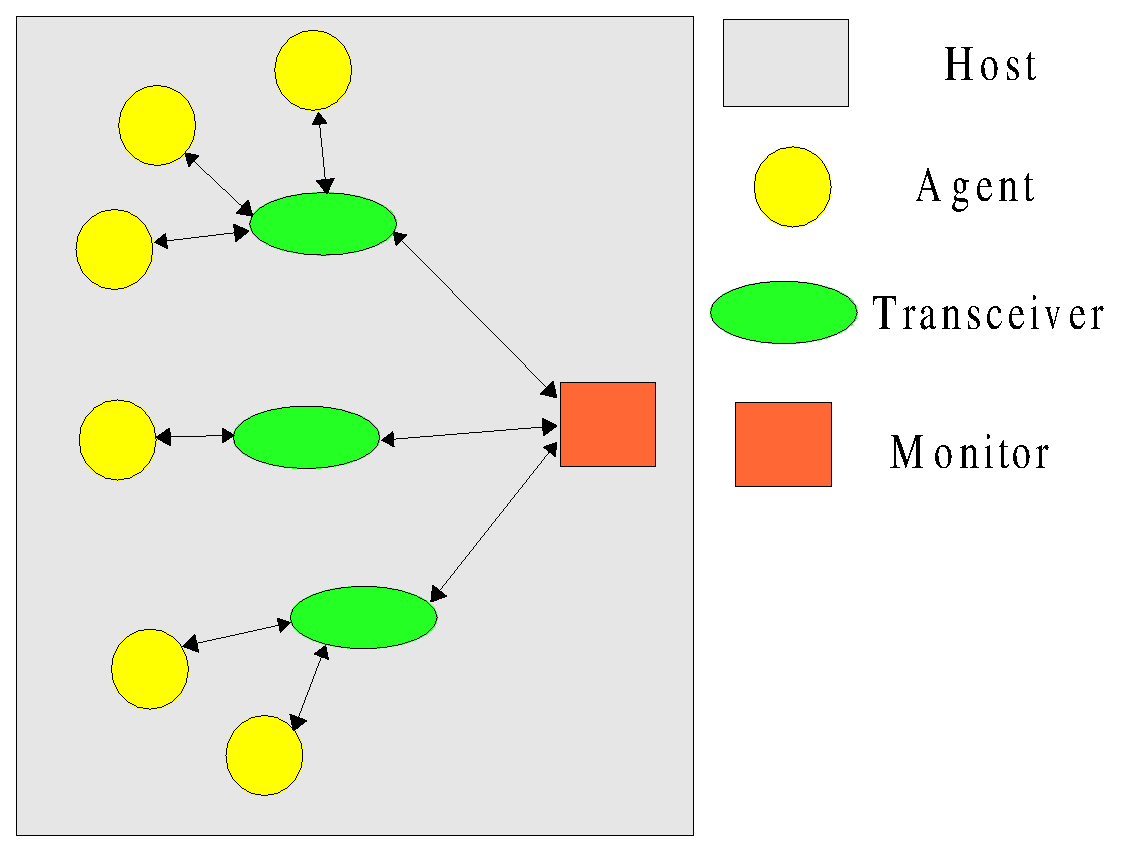
\includegraphics[scale=0.6]{AAFID-richtige-groesse.eps}
	\captionof{figure}{AAFID--Modell}
\end{center}
\vspace{1cm}

AAFID ist hierarchisch strukturiert. An unterster Stelle stehen die
Agenten. Es k"onnen mehrere Agenten, die jeweils unterschiedliche
Aufgaben haben, pro Host eingesetzt werden. Alle Agenten senden ihre
Informationen an einen Transceiver, der sich auf demselben Host
befindet. Der Transceiver "uberwacht und steuert die Agenten, er kann
sie starten, anhalten und rekonfigurieren. Zus"atzlich ist der Transceiver
noch f"ur die Datenreduktion verantwortlich und "ubergibt seine
Ergebnisse an einen oder mehrere Monitore, die die n"achst h"ohere
Instanz der Hierarchie darstellen. Die Monitore selbst k"onnen wieder
hierarchisch angeordnet werden. Sie kontrollieren die Daten von den
Transceivern und f"ugen sie zusammen. Die F"ahigkeit der Monitore, die
Daten von verschiedenen Hosts zu vereinigen, macht es m"oglich, dass
Attacken, die von mehreren Hosts ausgehen, erkannt werden k"onnen.
Der Aufbau von AAFID erlaubt eine leichte Skalierung. Wenn dem
Netz ein neuer Server hinzugef"ugt wird, m"ussen einfach nur die
AAFID-Komponenten installiert werden, die dann ihre Daten an einen
"ubergeordneten Monitor schicken.

\subsection{Analyseverfahren}

Bei den Analyseverfahren haben sich in den letzten Jahren drei Richtungen
herauskristallisiert. Die "alteste Methode, um Einbr"uche festzustellen,
ist \textit{Misuse Detection\/}. Bei diesem Verfahren wird ein Mustervergleich
(Pattern Matching) vorgenommen. Die Daten der Event--Box werden mit
Angriffsmustern (Attack Signatures) aus einer Datenbank verglichen.
Ist dieser Vergleich positiv, dann wurde eine Verletzung der Security
Policy erkannt und es wird entsprechend reagiert. Im kommerziellen
sowie im nichtkommerziellen Bereich ist \textit{Misuse Detection\/} immer noch
das am h"aufigsten benutzte Verfahren. Es ist einfach zu realisieren,
anzuwenden und nicht sehr anf"allig f"ur falsche Alarme (\textit{False Positives}).
Der gro"se Nachteil dieses Verfahrens ist, dass es nur bekannte Angriffe
erkennt, was zur Folge hat, dass neue Angriffe, die sich noch nicht
in der Signature--Datenbank befinden, keinen Alarm ausl"osen (False
Negatives) und somit unbemerkt bleiben.

Um dieses Defizit auszugleichen wurde ein neuer Weg eingeschlagen
und die \textit{Anomaly Detection\/} entwickelt. \textit{Anomaly Detection\/} geht davon
aus, dass alles was nicht zur Menge des \glqq normalen\grqq\/ Verhaltens geh"ort,
also demnach \glqq anomal\grqq\/ ist, ein Angriff sein muss. Diese
Methode hat gegen"uber \textit{Misuse Detection\/} den Vorteil, dass sie es erm"oglicht,
neue Angriffe zu erkennen, da sie ein abnormales Verhalten darstellen.
Zudem muss keine Datenbank mit Angriffsmustern aktualisiert und gepflegt
werden. Aber auch hier tauchen wieder Schwierigkeiten auf, die die
Verbreitung von \textit{Anomaly Detection\/} im kommerziellen Bereich stark behindern.
Verfahren zur Anomalieerkennung m"ussen zuerst das \glqq normale\grqq\/ Verhalten
eines Netzes oder Computersystems erlernen, indem sie Profile f"ur die
Benutzer und das System anlegen. Diese Phase an sich stellt schon eine
H"urde dar und k"onnte auch von einem Angreifer ausgenutzt werden, um dem
IDS Angriffe als normales Verhalten beizubringen. Das Intrusion--Detection--System k"onnte
somit zuk"unftige Angriffe dieser Art nicht mehr erkennen. Ein weiteres
Manko besteht in der hohen Rate an \textit{False Positives}, die durch St"orungen
in der normalen Systemaktivit"at ausgel"ost werden, aber keine Angriffe
darstellen. Zus"atzlich ist die Implementierung von \textit{Anomaly Detection\/}
gegen"uber der \textit{Misuse Detection\/} schwieriger, da die angewandten Verfahren
komplexer sind.

Ein noch sehr junges Verfahren, das als \textit{Burglar Alarm\/}, \textit{Passive Traps\/},
oder \textit{Strict Anomaly Detection\/} bezeichnet wird, benutzt einen relativ
simplen, jedoch sehr effektiven Ansatz. Es besagt, dass alles was nicht
\glqq richtig\grqq\/ ist, \glqq falsch\grqq\/ sein muss. Diese Aussage erinnert an Anomaly
Detection; es wird aber Mustererkennung wie bei \textit{Misuse Detection\/} benutzt,
d.h., das bekannte, normale Verhalten des Systems wird als
Signature in eine Datenbank abgelegt und jede Systemaktivit"at, die nicht einem
der Muster aus der Datenbank entspricht, ist anomales Verhalten und signalisiert
einen Angriff.
Es m"ussen nur relativ wenige Muster in der Datenbank abgespeichert werden.
Diese Muster m"ussen nicht wie bei \textit{Misuse Detection\/} f"ur jeden neuen Angriff
aktualisiert werden, sondern nur bei einer Ver"anderung des IT-Systems.
Dadurch ergibt sich ein geringer Verwaltungsaufwand im laufenden Betrieb als
bei normalen \textit{Misuse Detection\/} Systemen.

Damit das ganze etwas klarer wird, ein kleines Beispiel:
Der eMail--Proxy in einer DMZ darf nur TCP-Pakete auf Port 25
empfangen und absenden. Desweiteren d"urfen diese Pakete nur in das Internet
oder in das zu sch"utzende Netz geschickt werden. Das ist das \glqq richtige\grqq\/
Verhalten, welches als ein Muster in einer Datenbank abgelegt wird.
Das IDS "uberpr"uft nun den Paketfluss des eMail--Proxies mit dem gespeicherten
Muster. Sollte der eMail--Proxy diesem Verhalten einmal nicht folgen, so besteht
die Wahrscheinlichkeit eines Angriffs. Die Muster m"ussen sich nicht auf abstrakte
Netzverbindungen beziehen, sondern k"onnen auch tiefere Ebenen wie
Header--Informationen der einzelnen Netzwerkschichten oder Systemaufrufe eines
Betriebssystems widerspiegeln.

Damit die Fehlerquote bei der Erkennung von Angriffen vergleichbar
gering bleibt, m"ussen Anomalien, wie sie immer mal wieder in Netzwerken
auftreten, als Ausnahme explizit angegeben werden oder in einen Toleranzbereich
fallen. Somit k"onnen \textit{False Positives} zwar auftreten, sind aber weitaus
geringer als bei \textit{Anomaly Detection\/}, \textit{False Negatives} sind nahezu ausgeschlossen.
Wenn Angriffe unter der Toleranzgrenze bleiben, dann werden sie nat"urlich
nicht detektiert.

Nachfolgend sollen die verschiedenen Analyseverfahren f"ur Misuse und
\textit{Anomaly Detection\/} kurz erl"autert werden. Auf \textit{Strict Anomaly Detection\/}
und andere alternativen Analyseverfahren (Immunsystem, Genetische
Algorithmen, Datamining, etc.) soll hier nicht n"aher eingegangen werden, da sie noch
zu neu sind und bisher noch keine Verwendung in der Praxis finden.

\subsubsection{Mustererkennung}

\paragraph*{Experten Systeme}
F"ur die Analyse der Daten wurden schon fr"uh F"ahigkeiten von
Experten Systemen entdeckt. Folgende Intrusion--Detection--Systeme benutzten
Experten Systeme:
	\begin{itemize}
	\item MIDAS
	\item IDES
	\item NIDES \cite{www-nids}
	\item DIDS
	\item AID (benutzt RTworks) \cite{www-aid}
	\item Emerald (benutzt eine Abwandlung von P-BEST) \cite{www-emerald}
	\item CMDS (benutzt das freie System CLIPS \cite{www-clips})
	\end{itemize}

Experten Systeme k"onnen mit \textit{if-then-else-}Ausdr"ucken von dem
Anwender leicht programmiert werden. Sie haben aber das Problem,
dass sie gro"se Mengen dieser Regeln nicht schnell genug abarbeiten
k"onnen, da sie nur Interpreter, und damit bekanntlich langsam
sind. Hinzu kommt noch, dass ein Experten System nat"urlich immer
nur so gut sein kann, wie die Person, die es programmiert hat. Eine
Ver"anderung des Regelwerks gestaltet sich schwierig, da es
Auswirkungen auf die restlichen Regeln hat. Durch die reinen
\textit{if--then--else--}Bedingungen sind Experten Systeme nicht in der Lage
Unsicherheiten bzgl. der Angriffsanalyse zu handhaben, sondern
k"onnen nur \glqq Ja\grqq -- oder \glqq Nein\grqq --Aussagen machen.

\paragraph*{Zustandsautomaten (State Transition)}
F"ur \textit{Misuse Detection\/} bieten optimierte Zustandsautomaten zur
Mustererkennung eine flexible und leistungsf"ahige M"oglichkeit Eindringlinge
zu erkennen.

Das erste Intrusion--Detection--System, das diese Technik benutzte, war STAT \cite{www-stat}
und sp"ater USTAT, NetSTAT und WinSTAT, die alle an der Universit"at von
Californien, Santa Barbara, entwickelt wurden.
Auf dem ACM Workshop im Jahr 2000 wurde eine flexible und
kraftvolle Beschreibungssprache names STATL f"ur zustandsautomatenbasierte
Intrusion--Detection--Systeme, ebenfalls von der Universit"at
von Californien, Santa Barbara, vorgestellt.

\begin{center}
	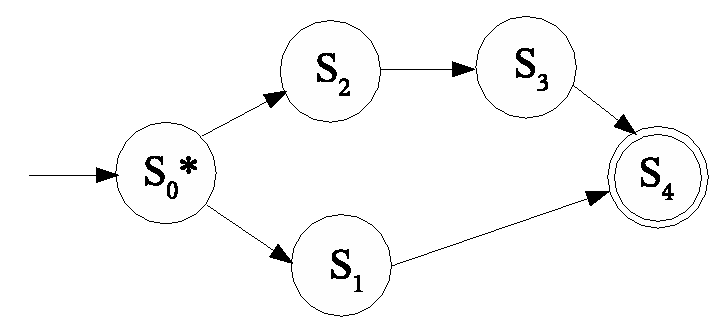
\includegraphics[scale=0.7]{State-Transition_new.eps}
	\captionof{figure}{Zustandsautomat}
\end{center}

Das obige Bild zeigt den Weg von einem Startzustand (Kreis \texttt{S$_{0}$}) "uber
mehrere \textit{Transitionen} und \textit{States\/} zu einem Endzustand
(Kreis \texttt{S$_{4}$}), der einen Einbruchsversuch signalisiert. Ein Eindringen
in das System besteht i.d.R. aus mehreren Aktionen. Jede Aktion wird durch eine
\textit{Transition\/} wiedergegeben. Die \textit{States\/} spiegeln den Systemzustand
wieder, der bspw. aus User--Privilegien, vorhandenen Dateien oder dem
derzeitigen Zustand eines Netz-- oder Systemdienstes bestehen kann.
Das Intrusion--Detection--System verwaltet f"ur jedes Angriffsszenario ein State--
Transition--Diagramm. Wenn eine Systemaktivit"at stattfindet,
"uberpr"uft die Analyseeinheit diese mit jedem State--Transition--Diagramm
und "uberf"uhrt jeden Zustandsautomaten in den neuen State,
wenn die Aktivit"at mit der Transition "ubereinstimmt. Dieses Verfahren
macht es m"oglich, die Wahrscheinlichkeit und den Verlauf von
Angriffen zu ermitteln und die Schritte des Angreifers vorherzusagen,
indem die verschiedenen Zustandsautomaten bzgl. ihres aktuellen
States untersucht werden. Wurde der Endzustand erreicht, d.h. ein
Eindringen liegt vor, so wird ein entsprechendes Ereignis von der
Intrusion--Response--Einheit (C--Box) ausgef"uhrt. Die
Zustandsdiagramme bieten ein abstraktes Abbild der
Angriffsmuster, sie sind somit leicht verst"andlich und unabh"angig
vom Format der Audit--Daten und technischen Details.
Zustandsautomaten stellen das Minimum an Aktivit"at f"ur einen Angriff
dar. Aus diesem Grund k"onnen Varianten einer Attacke schon mit
wenigen, kleinen Zustandsautomaten abgedeckt werden. Auf State--Transition
basierte Intrusion--Detection--Systeme erm"oglichen es sogar koordinierte und
stark verlangsamte Attacken zu erkennen. Eine verbesserte Variante der
State--Transition--Analyse wurde mit dem sog. Colored Petri (CP)--
Netz im IDIOT IDS implementiert.

\paragraph*{Beschreibungs-/Interpretersprachen}
Damit sich die Benutzung von Analyseeinheiten in Intrusion--Detection--Systemen noch
etwas einfacher gestaltet, wurden Sprachen zur Beschreibung von
Angriffsszenarien entwickelt.
Bekannte Beispiele sind:
\begin{itemize}
	\item RUSSEL
	\item STALKER
	\item N--Code
	\item Snort's Beschreibungssprache
	\item STATL
%	\item regul"are Ausdr"ucke
\end{itemize}

\vspace{0.5cm}

\subsubsection{Anomalieerkennung}

\paragraph*{Quantitative Analyse}
Es gibt verschiedene Arten der quantitativen Analyse, die gel"aufigste
ist die Schwellwerterkennung (\textit{Threshold Detection\/} oder auch
\textit{Threshold and Triggers\/} genannt). Bei der Schwellwerterkennung
werden System-- und Benutzeraktivit"aten mit Hilfe von Z"ahlern
dargestellt. Der Wert der Z"ahler ist bis zu einem gewissen Schwellwert
als normales Verhalten definiert, bei der "Uberschreitung dieses
Schwellenwertes, wird ein m"oglicher Angriff gemeldet. Als Beispiel
kann man sich vorstellen, dass ein Benutzer in den letzten zwei
Stunden drei Mal erfolglos versucht hat sich an ein System
anzumelden. Der Wert 3 ist in diesem Fall der Schwellwert und das
IDS reagiert, indem es z.B. den Benutzeraccount sperrt.
Als Erweiterung der Schwellwertanalyse wurde die \textit{heuristische
Schwellwert Analyse} entwickelt. Bei der \textit{heuristischen Schwellwert
Analyse\/} sind die Grenzwerte nicht starr sondern werden dynamisch
angepasst. In unserem Beispielfall w"urde der Grenzwert nicht statisch
auf 3 gesetzt werden, sondern w"are anhand des Einlogverhaltens des
Users in der Vergangenheit berechnet worden.
Der Grenzwert k"onnte bspw. aus der alten Anzahl von fehlerhaften
Logins, zuz"uglich einer Standardabweichung, errechnet werden.
Als weiteres quantitatives Analyseverfahren kann man noch die
Integrit"atspr"ufung (\textit{Target--Based Integrity Check\/}) nennen. Bei dieser
Methode wird die Ver"anderung von Systemobjekten (Dateien,
Programme, Hardware etc.), die sich eigentlich nicht ver"andern d"urfen,
"uberwacht. Das bekannteste Beispiel ist \textit{Tripwire\/}. \textit{Tripwire\/} "uberwacht
Dateien und Programme, indem es kryptographische Hashwerte (MD5
Algorithmus) von ihnen generiert, sie in einer Datenbank ablegt und
diese MD5--Hashwerte in regelm"a"sigen Zeitabst"anden mit den
Hashwerten der z.Zt. im System befindlichen Dateien bzw.
Programme vergleicht. Stimmen die Hashwerte nicht "uberein, so
wurde die entsprechende Datei oder das Programm ver"andert, z.B. indem sie von
dem Angreifer durch ein trojanisches Pferd ersetzt oder der Inhalt der
Passwort--Datenbank verf"alscht wurde. Die quantitativen Methoden
werden aber nicht nur zur Erkennung von Attacken benutzt, sondern
auch zur Datenreduzierung.
Die Eigenschaft, Systemattribute und Benutzerverhalten in Zahlen
auszudr"ucken, macht sich das NADIR IDS zunutze, um die redundanten
und nutzlosen Informationen in den Audit--Daten zu reduzieren. Die
NADIR--Entwickler stellten Benutzeraktivit"aten mit Hilfe von
Vektoren dar. Diese \textit{Profile--Vektoren\/} k"onnen f"ur die Experten
Systeme und f"ur die statistische Analyse benutzt werden.

\paragraph*{Statistische Messungen}
IDES und NIDES benutzen statistische Verfahren und waren die ersten
funktionierenden \textit{Anomaly Detection\/} Systeme (eigentlich sind es
hybride Intrusion--Detection--Systeme, da sie sowohl \textit{Misuse Detection\/} als auch
\textit{Anomaly Detection\/} benutzen).
Die Systeme verwalten eine Menge von statistischen Profilen, die
das Normalverhalten der Benutzer und der Systemkomponenten
beinhalten. Die Profile werden in periodischen Zeitabst"anden
aktualisert. Ein Sicherheitsversto"s wird gemeldet, sobald eine starke
Abweichung vom Normal--Profil auftritt.

Ein weiteres IDS, das auf statistische Messungen basiert, ist
Haystack. Haystack benutzt zwei Mengen von statistischen Profilen.
Eine Menge dient zum Vergleich des Benutzerverhaltens gegen"uber
Angriffsverhalten, die zweite Menge wird benutzt um eine
Abweichung vom Normalverhalten festzustellen. Mit statistischen
Verfahren k"onnen Angreifer erkannt werden, die sich als andere
Benutzer maskieren, indem sie deren Account benutzen. Da sich der
Angreifer anders verh"alt, als der Benutzer, dessen Account missbraucht
wird, wird das IDS darauf aufmerksam und alamiert den SO. Zudem
k"onnen auch v"ollig neue Angriffstaktiken und --methoden erkannt
werden, die ein System mit quantitativer Analyse nicht erkennen
w"urde. Der gro"se Nachteil vieler statistischer Verfahren ist die
Unf"ahigkeit im Echtzeitbetrieb zu arbeiten, was eine sofortige
Reaktion auf einen Angriff unm"oglich macht. Zur Zeit der Entwicklung
dieser Analysemethoden war der \textit{Batchmode--Betrieb\/} v"ollig
ausreichend, da sie f"ur die "Uberwachung von \textit{Mainframes\/} konzipiert
waren und es noch keine so ausgepr"agte Vernetzung gab.
Der Versuch, statistische Analysen f"ur Realtime--Intrusion--Detection--Systeme zu
verwenden, scheiterte an der hohen Performanz, die daf"ur n"otig war.
Hinzu kommt, dass statistische Messungen nur eine Aktivit"at und nicht
eine Abfolge von Aktivit"aten analysieren k"onnen. Diese Eigenschaft
schr"ankt die Verwendung solcher Systeme im Hinblick auf die Menge
der zu detektierenden Attacken stark ein, da die meisten Angriffe aus
einer Abfolge von Handlungen bestehen.

Die o.g. Verfahren basieren alle auf Annahmen bzgl. des normalen und
nicht--normalen Verhaltens eines Systems. Der Grenzwert, den das IDS
benutzt, darf nicht zu niedrig sein, um falsche Alarmierungen (False
Positives) zu vermeiden, was nur dazu f"uhrt, dass das IDS nicht mehr
beachtet wird. Andererseits darf der Grenzwert nicht zu hoch liegen,
so dass Angriffe nicht erkannt werden (\textit{False Negatives}).

Die folgenden Ans"atze ben"otigen keine Parameter f"ur den Grenzwert und
versuchen, die Nachteile der parameterbehafteten Analyseverfahren
auszugleichen.

\paragraph*{Regelbasierte Systeme}
Diese Systeme funktionieren im Grunde genau wie statistische
Systeme, mit dem einzigen Unterschied, dass Regeln anstatt Statistiken
benutzt werden. \textit{Wisdom and Sense\/} (W\&S) ist bspw. ein regelbasiertes IDS.
Die Regeln k"onnen bei W\&S entweder durch den Benutzer
eingegeben werden (um die \textit{Security Policy\/} darzustellen) oder es kann
die Regel aus alten Audit--Daten generieren.
Das \textit{Time--Based Inductive Machine} (TIM) IDS benutzt auch Regeln,
geht aber einen ganz anderen Weg als andere \textit{Anomaly Detection\/}
Systeme. Es fahndet nicht nach individuellen Ereignissen, sondern
"uberwacht deren zeitliche Abfolge. Eine Anomalie liegt vor, wenn die
zeitliche Abfolge von Systemereignissen nicht eingehalten wurde.

\paragraph*{Neuronale Netzwerke}
Neuronale Netzwerke k"onnen anomales Verhalten mit Hilfe von
adaptiven Lerntechniken erkennen und ben"otigen deshalb keine
Parameter, die durch den Benutzer vorgegeben werden m"ussen. Das
neuronale Netzwerk muss erst mit sauberen, d.h. nicht mit
Angriffsaktivit"aten verunreinigten, Daten trainiert werden. Aufgrund
dieser Lerneigenschaft stellen neuronale Netzwerke einen gro"sen Wert
f"ur die Anomalieerkennung dar. Leider lassen sich durch Benutzung
von Neuronalen Netzwerken nicht die Ursachen einer Anomalie
herausfinden. Dem SO kann nur das Vorhandensein eines
Sicherheitsversto"ses nicht aber dessen Grund gemeldet werden.
Um dieses Problem zu umgehen, werden neuronale Netzwerke
entwickelt, die sich nur auf einen Angriffstyp beschr"anken. Das
bedeutet, wenn das neuronale Netzwerk f"ur \textit{SYN--Flooding\/} feuert,
dann weiss man, um welchen Angriff es sich handelt. Diese L"osung "ahnelt
dann aber wieder der Mustererkennung.



%
%% Kapitel
%


%% Kapitel
\chapter{Konzept}
Um das Ziel zu erreichen unterschiedlichsten Umgebungen und Anspr"uchen gerecht werden zu k"onnen,
muss ein "au"serst modulares System geschaffen werden. Dabei sollen die einzelnen
Komponenten, wie sie im \textit{Common Intrusion--Detection--Framework\/} beschrieben werden,
als eigenst"andige Programme implementiert werden. Daten zwischen den Komponenten sollen "uber
ein TCP/IP Netzwerk oder lokal "uber FIFOs ausgetauscht werden.

Eine solche Architektur reicht aber noch nicht aus, um die gew"unschte Modularit"at zu
erf"ullen. Aus diesem Grunde sollen wichtige Funktionen aus den einzelnen IDS--Komponenten
entnommen und in dynamisch ladbare Module ausgelagert werden.
Die Module sind einfach auszutauschen, und man umgeht das l"astige
und fehleranf"allige Anpassen des Quellcodes. Somit ist es nicht nur m"oglich, sich einer
gegebenen IT--Infrastruktur besser anpassen zu k"onnen, bspw. durch ein Datenbank--Modul f"ur
eine bereits vorhandene \textsc{Oracle} Datenbank, sondern es ist auch m"oglich, eigene
Verfahren in ein bestehendes System zu integrieren, um es zu verbessern oder einfach nur,
um seine eigenen Entwicklungen zu testen.

Das IDS soll unter SuSE Linux entwickelt und implementiert werden. Bei der Entwicklung
soll aber auf Portabilit"at geachtet werden, um sp"atere Portierungen zu vereinfachen.


\section{Audit--Datenquelle}
Jedes IDS lebt von den Daten, die es f"ur seine Analyse ben"otigt.
Hostbasierte Intrusion--Detection--Systeme analysieren i.d.R. Log--Daten
von Applikationen und dem Kernel.

In Applikations--Logs lassen sich anhand von Fehlermeldungen m"ogliche Angriffe
erkennen. Aber nicht nur direkte Attacken k"onnen erkannt werden, sondern
auch simple Verst"o"se gegen die Sicherheitspolitik. Beispielsweise k"onnte
das erfolgreiche Anmelden eines Administrators mitten in der Nacht, au"serhalb
der normalen Arbeitszeiten, ein Hinweis auf den Missbrauch des Administrator--Accounts
sein.

Leider sind Applikations--Logs oft nicht aussagekr"aftig genug, deshalb lassen sich
Angriffe auf Kernel--Ebene besser erkennen. Mit Hilfe
von Informationen "uber Systemaufrufe, wie der R"uckgabewert, die Identit"at des
Aufrufers, der Aufrufsequenz, die Parameter oder einfach aufgrund des Vorhandenseins
eines bestimmten Systemaufrufes lassen sich konkrete Aussagen "uber das
Verhalten von Benutzern und Applikationen machen.

Da Linux von Haus aus keine M"oglichkeit bietet Systemaufrufe \footnote{inzwischen gibt es ab
SuSE--Kernel 2.4.19 das \textit{Linux Trace Toolkit\/}, um das System auf Kernel--Ebene zu "uberwachen}
im \textit{User Space} zu verfolgen, soll ein eigenes \textit{Loadable Kernel Module\/}
(LKM) entwickelt werden, das diese Aufgabe erf"ullt.

Um die Log--Daten aus dem Kernel vor Manipulation zu sch"utzen, soll nicht der Umweg "uber \textit{Syslog}
oder andere Systemapplikationen gegangen werden. Eine eigene Ger"atedatei (Schnittstelle im
Dateisystem zwischen \textit{User Space} und \textit{Kernel Space})
soll im Linux--Dateisystem angelegt werden, die es Benutzerprogrammen erlaubt, die Daten mit \texttt{read(2)}
direkt aus dem \textit{Kernel Space} zu lesen. Diese Ger"atedatei soll nicht nur dazu dienen
Daten aus dem LKM zu lesen, sondern sie soll auch als Schnittstelle zur Steuerung des LKMs mit Hilfe von
\texttt{ioctl(2)} genutzt werden. Es soll m"oglich sein, das
Logging f"ur bestimmte Systemaufrufe an-- oder abzuschalten und den Status diverser, modulinterner Parameter
(Syscall--Status, Debug--Level, Ringpuffergr"o"se) in Erfahrung zu bringen.

Unser IDS soll also Textdateien in denen Log--Daten enthalten sind, "uberwachen
k"onnen und zudem eine Ger"atedatei auslesen, um Informationen aus dem Kernel
zu bekommen.

Da u.U. sehr viele Daten von dem LKM generiert werden k"onnten, muss man sich folgende Frage stellen:
\glqq Wohin mit all den Audit--Daten, wenn niemand sie aus dem \textit{Kernel Space} holt?\grqq\/
Es gibt f"ur ein solches Problem nur zwei L"osungen: Entweder man vergr"o"sert dynamisch den Puffer,
in dem man die Daten zwischenspeichert, oder man hat einen festen Speicherbereich und "uberschreibt
alte Eintr"age.

Der erste Ansatz hat den Nachteil, dass der ganze Kernel--Speicher aufgebraucht werden k"onnte, was zur Folge
h"atte, dass das System stehen bliebe. Der zweite Ansatz l"oscht Daten, die vielleicht wichtig f"ur die
Analyse sind.

F"ur unsere Implementierung soll der letzte Ansatz gew"ahlt werden. Die Daten werden in einem Ringpuffer
gespeichert, so dass immer die "altesten mit den neusten Eintr"agen "uberschrieben werden.

%Alle n"otigen Infomationen m"ussen vom LKM erfasst und weitergeleitet werden.
%Zudem muss das LKM "uber entsprechende Tools konfiguriert werden k"onnen um die Liste der
%zu "uberwachenden Syscalls ver"andern zu k"onnen.

Desweiteren muss das LKM selber vor Manipulation
gesch"utzt werden. Es soll die Option geschaffen werden, das LKM vor den Augen des Angreifers
zu verstecken und es fest im System zu verankern, so dass es nicht mehr entfernt werden kann.
Um die Verarbeitung der Informationen zu erleichtern, soll das LKM ein einfach zu analysierendes
Log--Format mit festen \textit{Tokens\/} und \textit{Delimitern\/} benutzen.

\section{Datenverarbeitung auf dem Client}
Die Log--Zeilen k"onnen Daten enthalten, die vom Benutzer beeinflusst wurden, aus diesem Grund m"ussen
beim Design der Client--Komponente von \textsc{M--ICE} entsprechende Sicherheitsvorkehrungen
getroffen werden. Die Client--Komponente soll nur da, wo es wirklich n"otig ist, mit Super--User--Rechten
arbeiten, zudem sollen, wenn immer m"oglich, logisch zusammengeh"orige Codeteile in eigene Prozesse
aufgespalten werden.

Die auf dem Client generierten Daten m"ussen auf sicherem Wege an andere IDS--Komponenten
f"ur die Weiterverarbeitung verteilt werden.
Dazu sind folgende Aufgaben n"otig:
\begin{itemize}
	\item Sammlung
	\item Filterung
	\item Pseudonymisierung
	\item Formatierung
	\item Verschl"usselung
	\item Weiterleitung
\end{itemize}

Die Filterung, Pseudonymisierung und Formatierung der Log--Daten soll jeweils in ein eigenes
Modul ausgelagert werden, da diese wichtigen Aufgaben durch verschiedenste Methoden realisiert
werden k"onnen.

\paragraph*{Sammlung} Das Sammeln von Audit--Daten soll darin bestehen, immer die aktuellste
Textzeile aus einer Log--Datei zu lesen. Dabei kann die Datei eine normale Datei, eine Ger"atedatei
oder ein FIFO sein. Somit k"onnen also \textit{Syslog}--Dateien, Applikations--Log--Dateien und bspw.
die Ger"atedatei des LKMs als Datenquelle dienen.

\paragraph*{Filterung} Die Filterung soll als erstes in der langen Kette der Datenverarbeitung
greifen, um die Menge der zu analysierenden und zu speichernden Daten zu reduzieren.
%Positiver Nebeneffekt ist neben der Datenreduzierung die Einsparung von Verarbeitungszeit.

Eine effiziente Datenreduktion, wie bspw. durch Abstraktion der Audit--Daten in Vektoren (s. NADIR IDS),
hat den Nachteil, dass die originalen Audit--Daten nicht weiter in der Analyse, und, noch
viel wichtiger, nicht mehr im Management--Teil des Intrusion--Detection--Systems auftauchen.
F"ur \textsc{M--ICE} sollen regul"are Ausdr"ucke vom Anwender in das System eingegeben
werden k"onnen, um Audit--Daten zeilenweise zu filtern. Diese Methode ist einfach zu implementieren,
ausreichend effektiv und verf"alscht zudem die Daten nicht. Als kleiner Nachteil hierf"ur sei
zu bedenken, dass der Adminitrator sein System kennen muss, um entscheiden zu k"onnen, welche
Log--Daten unwichtig sind und welche nicht.

\paragraph*{Pseudonymisierung} Die Pseudonymisierung von benutzerbezogenen Daten steckt
sozusagen noch in den Kinderschuhen. Pseudonymisierung wird aus Datenschutzgr"unden eingesetzt
und ist nicht zu verwechseln mit Anonymisierung. Bei der Anonymisierung wird bspw. die Identit"at
einer Person so ver"andert, dass es nicht mehr m"oglich ist festzustellen, welche reale Person sich
hinter einer anonymisierten Identit"at verbirgt. Diese Technik macht den Einsatz im
Intrusion--Detection--Bereich
nutzlos, da man nat"urlich wissen m"ochte, wer hinter einem Sicherheitsversto"s steht.
Die Pseudonymisierung erlaubt es hingegen, die Privatssph"are von Computerbenutzern zu sch"utzen
und gleichzeitig diese Privatssph"are wieder aufzuheben, sobald ein Angriff entdeckt wurde.

Zwei in Deutschland entwickelte Verfahren sind recht bekannt und wurden gr"o"stenteils auch schon
implementiert.

An der Universit"at Cottbus wurde im Laufe der Entwicklung des Intrusion--Detection
Systems AID \cite{www-aid} von M. Sobirey et al. ein Verfahren zur Pseudonymisierung mit Hilfe von
symmetrischer Krypthographie entwickelt. Dabei wird auf dem zu beobachteten Rechner mit
einem geheimen Schl"ussel die Benutzeridentit"aten chiffriert. Wird ein Angriff erkannt, dann wird die
verschl"usselte Benutzeridentit"at mit dem geheimen Schl"ussel wieder in Klartext "ubersetzt.

Eine andere Methode wurde von U. Flegel an der Universit"at Dortmund entwickelt. Hier wurde
ein anderer kryptographischer Ansatz benutzt, das sog. \textit{Secret Sharing\/} (s. \cite{book-crypto-1},
S. 84 ff.). Beim \textit{Secret Sharing\/} wird ein geheimer Schl"ussel in n Teile aufgebrochen.
Diese n Schl"usselteile ben"otigt man, um Ciphertext wieder in Klartext umwandeln zu k"onnen.
Man definiert also einen Schwellwert und nur wenn diese Schwelle "uberschritten wird
kann die Identit"at eines Benutzers wieder hergestellt werden. Zum besseren Verst"andnis
ein kleines Beispiel: Die Sicherheitspolitik erlaubt drei fehlgeschlagene Login--Versuche, bevor
der Administrator benachrichtigt wird. Der Schwellwert liegt also bei drei und somit m"ussen
auch drei \textit{Shared Secrets\/} generiert werden. Wurden vom System drei Fehlermeldungen erzeugt,
so ist es m"oglich, die Identit"at des Benutzers wieder herzustellen.

F"ur \textsc{M--ICE} soll kein Pseudonymisierungsverfahren implementiert werden, um den Entwicklungsaufwand
gering zu halten. Es soll jedoch durch ein Modul in der Client--Anwendung von \textsc{M--ICE}
die M"oglichkeit geschaffen werden, ein solches Verfahren sp"ater problemlos einzuf"uhren.

\paragraph*{Formatierung} Die nativen Unix--Log--Daten sollen mit weiteren Informationen
angereichert und in ein einheitliches Format gebracht werden. Folgende zus"atzliche
Informationen k"onnen n"utzlich sein:
\begin{itemize}
	\item Rechnername
	\item Domainname
	\item IP--Adresse
	\item Betriebssystem
	\item Betriebssystem--Release
	\item Betriebssystem--Version
	\item Datum
	\item Uhrzeit
\end{itemize}


\paragraph*{Verschl"usselung} Die Verschl"usselung auf dem Client soll mit Hilfe eines symmetrischen
Verschl"usselungsverfahrens geschehen. Bei symmetrischer Kryptographie in verteilten Systemen besteht das
Problem der Schl"usselverteilung. Im Fall von \textsc{M--ICE} reicht es aus, wenn der Administrator
den geheimen Schl"ussel in die entsprechende Konfigurationsdatei eintr"agt.

\paragraph*{Weiterleitung} Die verschl"usselten Daten m"ussen in zwei Richtungen weitergeleitet werden:
zur Analyseeinheit und an eine Datenbank zur Speicherung. Da die Verdopplung des Datenstroms u.U. dazu
f"uhren kann, dass das Netzwerk "uberlastet wird, sollen entsprechende Optionen bereitgestellt werden,
diesem bei Bedarf entgegen wirken zu k"onnen.

\section{Analyse}
Es ist nicht Ziel der Diplomarbeit, ein besonders ausgefeiltes Analyseverfahren zu implementieren
oder sogar zu entwickeln. Dies w"urde den Umfang einer eigenen Diplomarbeit in Anspruch nehmen.
Um das System aber testen zu k"onnen, soll eine einfache Analyse mit Hilfe von regul"aren Ausdr"ucken
implementiert werden.

Der Quellcodeteil, der die Analyse durchf"uhrt, wird in ein Modul ausgelagert. Dieses Modul soll
umfassend konfigurierbar sein, damit ausreichend Flexibilit"at geboten wird, die sogar eine Zusammenschaltung
der Analyseverfahren erlaubt.

Analyseergebnisse, die an den Management--Host oder an eine andere Analyseeinheit weitergereicht werden,
sollen im \textit{Intrusion Detection Message Exchange Format\/} eingepackt und verschl"usselt werden.


\section{Datenbanken}
Das System soll "uber zwei Datenbanken verf"ugen. Eine Datenbank dient zur Speicherung von
rohen \textit{Syslog}--Daten und analysierten Kernel--Daten, um eine genauere, manuelle Analyse
bei verd"achtigen Handlungen durchf"uhren zu k"onnen. Die zweite Datenbank speichert
lediglich die gemeldeten Alarme und die entsprechende IDMEF--Nachricht.

Zur Bewahrung der Datenintegrit"at sollen die Log--Daten an der Quelle kryptographisch
signiert werden. So gespeicherte Daten lassen Manipulationen leicht erkennen und geniessen
zudem einen h"oheren Echtheitswert, um bspw. auch in juristischen Auseinandersetzungen genutzt
werden zu k"onnen.


\section{Management--Host}
Der Management--Host soll Alarme von verschiedenen Analyseeinheit in unterschiedlichen Formaten
entgegennehmen k"onnen und benutzerdefinierte Reaktion ausl"osen.

Damit der Management--Host Ereignisse von verschiedenen Sensoren verwalten kann, muss eine
Tabelle f"ur die Zuordnung zwischen Klassifikation und Klassifikationsbeschreibung und eine
Tabelle zur Abbildung der Alarme auf vorhandene Reaktionen existieren.

Kleine und leicht austauschbare Programme sollen die Reaktionen des Systems "ubernehmen. Dabei
soll die M"oglichkeit bestehen, Reaktionen ohne Probleme hinzuzuf"ugen oder zu entfernen.

Zus"atzlich sollen Schnittstellen geschaffen werden, um andere IDS Sensoren, bspw. Snort \cite{www-snort},
mit dem Management--Host verwalten zu k"onnen. Diese Eigenschaft w"urde den Aufbau eines hybriden
Intrusion--Detection--Systems erlauben.


\section{Heartbeat}
Die Komponenten des Intrusion--Detection--Systems sollen an dem Management--Host ihren Prozessstatus melden,
damit festgestellt werden kann, ob ein Prozess eingefroren oder sogar beendet wurde. Dieses kann absichtlich
durch einen Angreifer geschehen sein oder auch unabsichtlich durch Fehler oder "Uberlastung des Client--Systems.
Hierf"ur soll die IDMEF--Heartbeat--Klasse benutzt werden.

Der Management--Host muss eine Liste mit allen Komponenten verwalten, die je eine Heartbeat
Nachricht gesendet haben oder noch senden m"ussen. F"allt eine Einheit aus, so bleibt auch die
Heartbeat--Nachricht aus und der Management--Host kann den Security Officer entsprechend
dar"uber informieren.


\section{Graphical User Interface}
Damit der Benutzer die erkannten Angriffe besser "uberschauen und weiterverarbeiten kann,
soll die Benutzung eines \textit{Graphical User Interfaces\/} (GUI) ber"ucksichtigt werden;
es soll jedoch keine GUI implementiert werden, da auch diese Aufgabe den Umfang dieser
Diplomarbeit "uberschreiten w"urde. Einer m"oglichen GUI m"ussen also gen"ugend Schnittstellen
und Informationsquellen zur Verf"ugung gestellt werden, damit der Benutzer mit allen wichtigen
Daten versorgt werden kann. Als Informationsquelle k"onnte bspw. eine SQL--Datenbank oder im XML--Format
gespeicherte Daten dienen.


\section{Verschl"usselte Kommunikationsprotokolle}
Die Kommunikation "uber das Netzwerk soll verschl"usselt erfolgen, um die Daten und die Komponenten
zu sch"utzen. Oberster Leitsatz hierbei ist jedoch, alles einfach zu halten, um eventuelle
logische Fehler im Design der Protokolle zu vermeiden.

Damit die Prozesse des Intrusion--Detection--Systems nicht unn"otig ausgebremst oder aufgebl"aht werden,
soll f"ur die Verschl"usselung ein symmetrischer und kein asymmetrischer Algorithmus benutzt werden.
Eine Schl"usselverteilung \`a la \textit{Kerberos\/} \cite{www-kerberos} oder \textit{Needham-Schroeder\/}
\cite{www-needham} soll nicht eingesetzt werden. Die manuelle Schl"usselverteilung ist v"ollig ausreichend.
Gl"ucklicherweise verlieren die "ubermittelten Daten ihren Wert innerhalb einiger Sekunden
(Dauer der Verarbeitung durch die IDS--Komponenten).

Kommunikationsprotokolle werden bei jeder Transaktion von Daten zwischen allen Prozessen, egal
ob lokal oder entfernt, benutzt. Verschl"usselung ist hingegen aber nur n"otig, wenn die Daten
"uber ein Netzwerk an ein entfernten Prozess geschickt werden. Sollten die Daten bspw. "uber ein
\textit{Loopback Device\/} gehen, muss dem Anwender die M"oglichkeit bleiben, die Verschl"usselung
abzuschalten.

Bei der Verschl"usselung der Daten wurden drei Ziele verfolgt:
\begin{itemize}
	\item Schutz vor Manipulation
	\item Schutz vor unbefugtem Lesen
	\item Schutz gegen \textit{Replay Attacken\/}
\end{itemize}

\paragraph*{Manipulation} Die Manipulation unserer Audit--Daten w"urde unweigerlich dazu f"uhren,
dass wir nach dem Entschl"usseln unbrauchbare Daten erhielten. Das Resultat w"are zum einen
fehlerhafte Eintr"age in unseren Datenbanken und zum andern, was wesentlich schlimmer
ist, wird die Analyse dadurch gest"ort.
Um dem zu entgegnen muss eine Pr"ufsumme von unserem Klartext berechnet werden. Diese
Pr"ufsumme wird mit dem Klartext verschl"usselt und muss vom Kommunikationspartner validiert
werden.

\paragraph*{Lesen} Das Lesen unserer Daten muss mit Hilfe von Kryptographie verhindert werden, um
einem Angreifer die M"oglichkeit zu nehmen, in Erfahrung zu bringen, was das IDS sieht und erkennt.
Zudem ist die Verschl"usselung zwingend notwendig, um die o.g. Manipulation zu verhindern.
% und das Ausf"uhren der Gegenma"snahmen mit Hilfe des \textit{ReactionDaemon\/}
%zu sichern.
%
%Bei der Verwendung von Kryptographie in \textsc{M-ICE} geht es nicht darum die Daten bis in alle Ewigkeit geheim
%zu halten, da die Log--Daten, nachdem sie ausgewertet wurden, keinen gro"sen Wert mehr besitzen.
%F"ur die Krypthographieunterst"utzung wurde die MCrypt-Bibliothek (\cite{www-libmcrypt}) benutzt.

\paragraph*{Replay Attacken} Ein potentieller Angreifer kann \textit{Replay Attacken} (s. \cite{book-crypto-1}, S. 70)
dazu benutzten, die Analyseeinheit unseres Intrusion--Detection--Systems durcheinander zu bringen, Eintr"age
in den Datenbanken vorzunehmen oder sogar, um Reaktionen ausf"uhren zu lassen.

Die einfache Verschl"usselung der Nachricht hilft hier nicht gegen einen Angriff auf das Protokoll.
Da immer der selbe Schl"ussel benutzt wird, kann eine aufgezeichnete Nachricht sp"ater wieder
eingespielt werden und w"urde vom IDS akzeptiert und verarbeitet.

Es gibt mehrere L"osungsans"atze, um \textit{Replay Attacken\/} zu verhindern. F"ur unser IDS wird
einfach ein Zeitstempel benutzt. Vorrausetzung hierf"ur ist aber, dass auf allen beteiligten Rechnern
die Zeit synchronisiert wird bspw. "uber NTP. Da das Paket von Applikationsebene zu Applikationsebene
jedoch etwas Zeit ben"otigt muss der Empf"anger ein Zeitfenster erlauben, in dem ein Paket ankommen darf.
Dieses Fenster ist aber nur f"ur das erste Paket n"otig, nachfolgende Pakete m"ussen immer einen h"oheren
Zeitstempel haben als das vorherige. Dieses Fenster erlaubt immer noch einen \textit{Replay Angriff\/}
mit dem ersten Paket; die Angriffsfl"ache wird jedoch verkleinert. Da diese L"osung nicht absolut
wasserdicht ist, muss eine Verbesserung vorgenommen werden.

Mit einigen Ver"anderungen lie"se sich die Gefahr einer \textit{Replay Attacke\/} noch
weiter verringern. Beispielsweise k"onnte das erste Paket ausschlie"slich zur Zeitsynchronisation
benutzt werden und keine weiteren Daten enthalten. Damit k"onnte ein Angreifer aber immer noch
die ganze Verbindung inkl. Zeitsynchronisationspaket duplizieren, um sein Ziel zu erreichen.
So ein Angriff ist aber nur m"oglich, wenn der Server multi--threaded, also parallel, l"auft. Ein
parallel laufender Server sollte also noch Absenderadresse und Absenderport in einer globalen
Tabelle f"ur aktive Client--Sessions verwalten und bei neuen Verbindungen diese Werte pr"ufen.

F"ur unser IDS wurde jedoch ein viel einfacheres und dennoch effektives Mittel gegen
\textit{Replay Attacken} gefunden. Zwischen den parallelen Clientverbindungen soll einfach
eine bestimmte Zeit (Zeitfenster + n) gewartet werden, so dass der Zeitstempel wiedereingespielter
Pakete auf jedenfall zu alt ist.


%
%% Kapitel
%
\chapter{Implementierung}

\section{Intrusion Detection Message Exchange Format}

Das \textit{Intrusion Detection Message Exchange Format\/} (IDMEF \cite{draft-idmef}) ist ein
von der \textit{Intrusion Detection Working Group\/} (IDWG \cite{www-idwg}) entwickeltes
objektorientiertes Datenformat. IDMEF basiert auf \textit{Unified Modeling Language\/} (UML)
und \textit{Extensible Markup Language\/} (XML), um ein erweiterbares, aber dennoch
einheitliches Format definieren zu k"onnen.

IDMEF wurde entwickelt, um Informationen zwischen einem IDS--Sensor und dem IDS--Manager
auszutauschen. Aber man kann es auch benutzen, um bspw. Alarme von verschiedenen Intrusion--Detection--Systemen
in einer einzigen Datenbank zu sammeln, zu korrelieren oder mit Hilfe eines \textit{Graphical User Interface\/}
darzustellen.

\subsection{IDMEF--Message--Aufbau}
UML bietet die M"oglickeit, Beziehungen zwischen Klassen aufzuzeigen und stammt eigentlich
aus der Softwareentwicklung. Eine Klasse besteht aus einem Namen und aus Attributen, dabei
m"ussen Attribute nicht zwingend angegeben werden.
Klassen werden wie folgt dargestellt:

\begin{center}
	
\includegraphics[scale=0.8]{UML-Klasse.eps}
	\captionof{figure}{UML Klasse}
\end{center}

Im UML Schema werden folgende Mengenangaben definiert:
\begin{itemize}
	\item \textbf{n}: genau n (ohne Angabe: 1)
	\item \textbf{0..*}: Null oder mehr
	\item \textbf{1..*}: Eins oder mehr
	\item \textbf{0..1}: Null oder Eins (oder auch \glqq optional\grqq)
	\item \textbf{n..m}: von n bis m (einschlie"slich)
\end{itemize}

\vspace{1cm}

Das IDMEF--Modell benutzt lediglich die Beziehungen Vererbung und Gruppierung.
Bei der Vererbung gibt es eine Oberklasse und eine beliebige Anzahl von Unterklassen.
Eine Unterklasse erbt alle Attribute, Operationen und Beziehungen der Oberklasse. Sie ist
aber in der Lage weitere Operationen oder Attribute zu definieren.
\begin{center}
	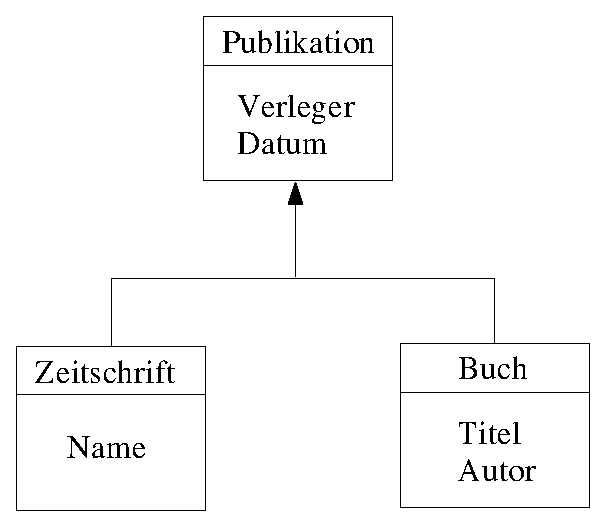
\includegraphics[scale=0.8]{UML-Vererbung.eps}
	\captionof{figure}{UML Vererbung}
\end{center}

\vspace{1cm}

Eine Gruppierung ist eine Vereinigung von Klassen. Dabei sind die einzelnen Klassen und deren
Attribute Teil der Gruppierungsklasse.
\begin{center}
	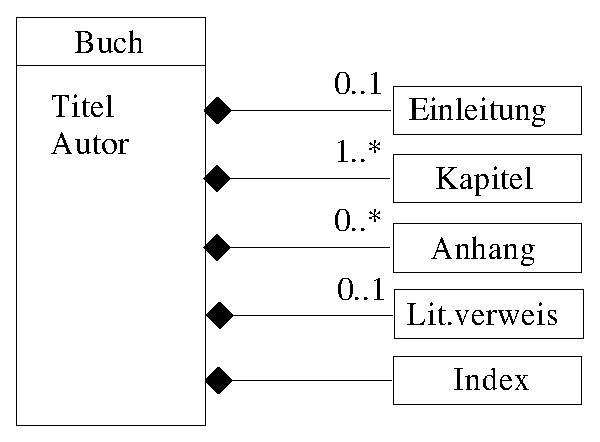
\includegraphics[scale=0.8]{UML-Gruppierung.eps}
	\captionof{figure}{UML Gruppierung}
\end{center}

\vspace{1cm}

Eine komplette IDMEF-Nachricht ist wie folgt aufgebaut:
\begin{center}
	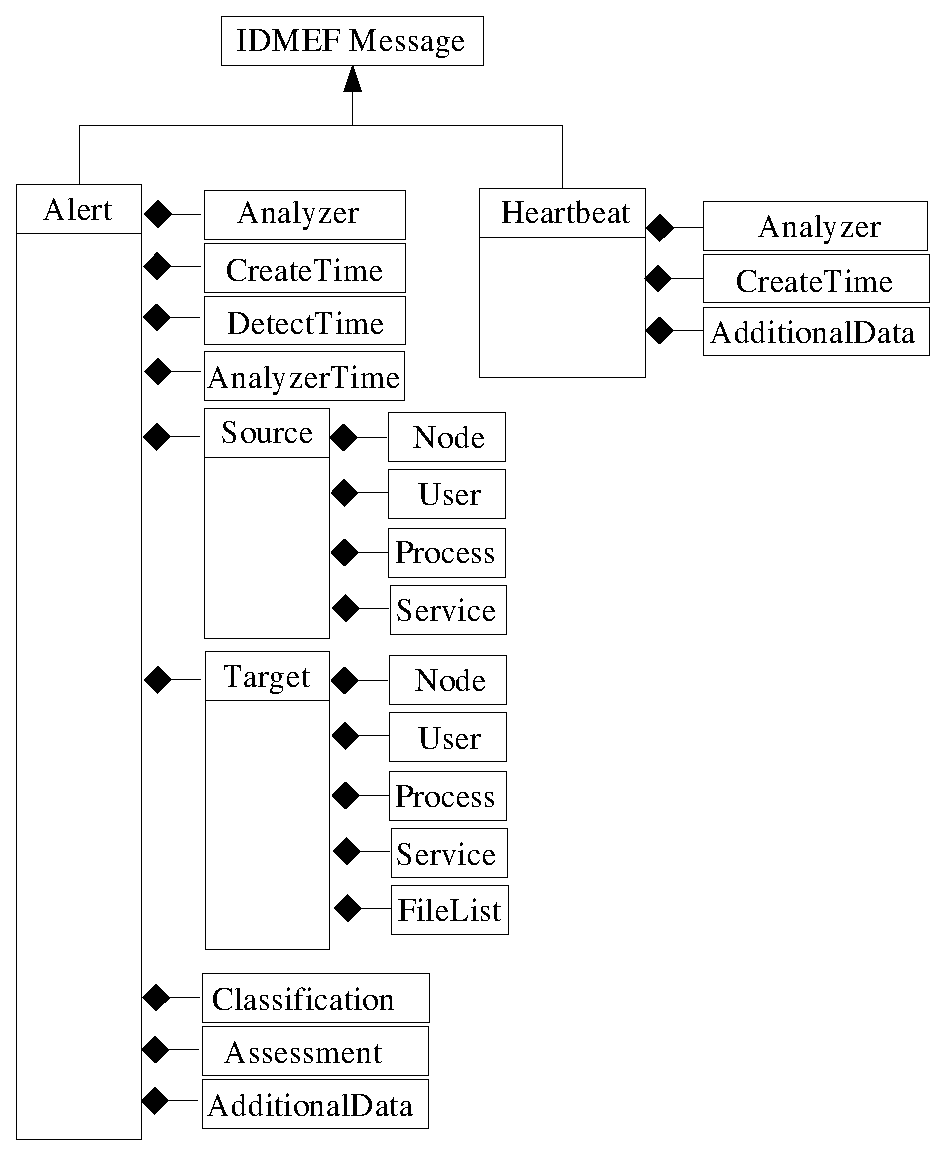
\includegraphics[scale=0.8]{IDMEF-Aufbau.eps}
	\captionof{figure}{IDMEF--Aufbau}
\end{center}


\section{Design}
Um die geforderte Modularit"at in Bezug auf dynamisch ladbare Module zu erf"ullen, kann unter
Linux die Funktion \texttt{dlopen(3)\/} benutzt werden. Diese Funktion dient prim"ar zum Laden
von \textit{Shared Libraries\/}, kann aber hervorragend f"ur unsere Zwecke benutzt werden.
Leider verwenden die unterschiedlichen Unix--Derivate ebenso
unterschiedliche Verfahren, um \textit{Shared Libraries\/} einzubinden. Aus diesem Grund
wird die Bibliothek \textit{libltdl\/} des \textit{libtool Projektes\/} von GNU \cite{www-libtool}
benutzt, um die Portabilit"at zu wahren.

Zur Unterst"utzung des IDMEF--Models wurde die \textit{libidmef\/} Bibliothek von
\textsc{SiliconDefense\/} \cite{www-libidmef} benutzt.
Diese Bibliothek stellt eine C--API zur Verf"ugung, um die IDMEF--Dokumente quasi objektorientiert
erzeugen und handhaben zu k"onnen. Leider fehlt hier die Implementierung eines geeigneten
Transportprotokolls (bspw. IAP und IDXP) \footnote{\textit{libiap} \cite{www-libiap} und
\textit{libidxp} \cite{www-libidxp} wurden sp"ater entdeckt und nicht mehr verwendet},
so dass ein eigenes Protokoll entwickelt werden musste.

Der detaillierte Aufbau von \textsc{M-ICE} soll mit Hilfe des folgenden Diagramms verdeutlicht werden.
\vspace{1cm}
\begin{center}
	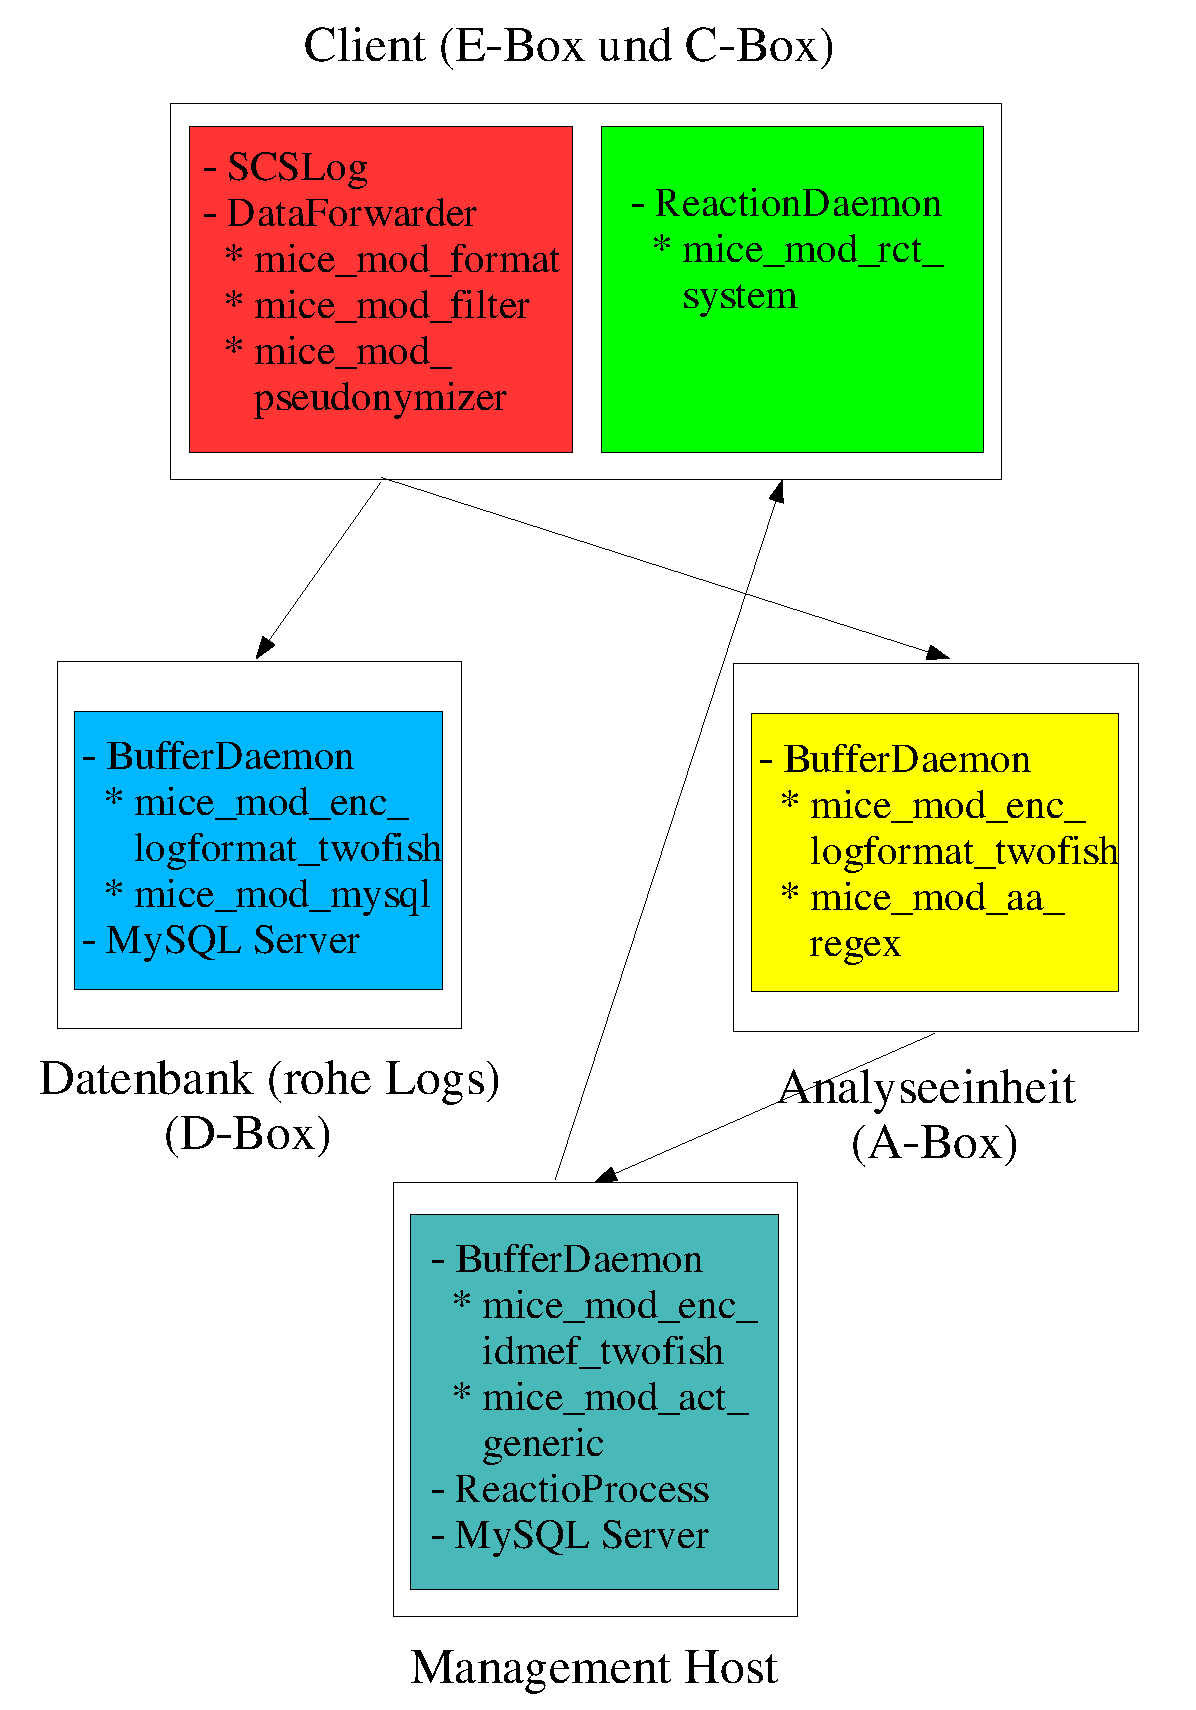
\includegraphics[scale=0.5]{MICE-Aufbau_02.eps}
	\captionof{figure}{Detaillierter Aufbau von M--ICE}
\end{center}
\vspace{1cm}

\pagebreak

Stark abstrahiert stellt das ganze also einen Kreislauf dar. Der Kreis beginnt mit einer Aktion
auf dem Client, diese Aktion wird im Verlauf des Kreises analysiert und die Reaktion auf dem Client
schlie"st den Kreis wieder.
\begin{center}
 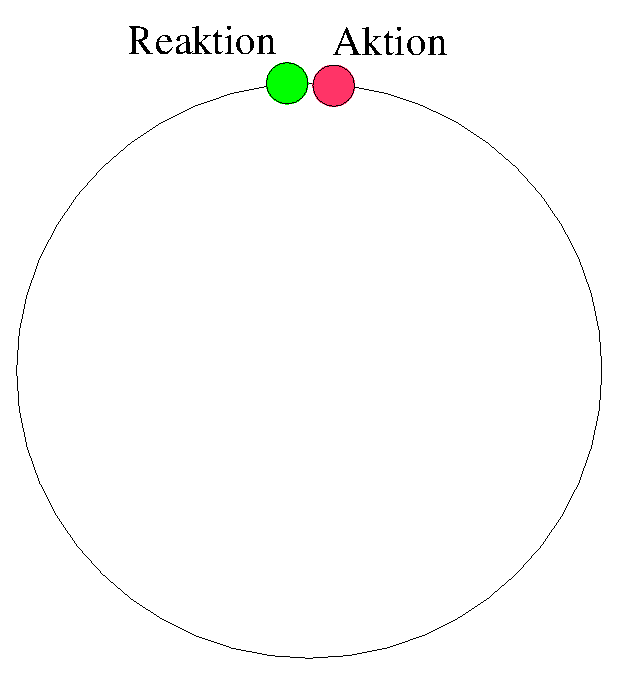
\includegraphics[scale=0.39]{MICE-Aufbau_03.eps}
	\captionof{figure}{Abstrakter Aufbau von M--ICE}
\end{center}


\subsection{Die Bausteine}
%Die Verteilung der Komponenten sollte nun klar sein.
Nachfolgend soll die Implementierung genauer betrachtet werden.

\subsubsection{SCSLog --- Das Kernel--Modul}
Da Linux von Haus aus kein Syscall--Logging unterst"utzt, wurde ein \textit{Loadable Kernel Module\/}
(LKM) entwickelt, welches dieses erm"oglicht. Der Aufbau sieht wie folgt aus:
\vspace{0.5cm}
\begin{center}
	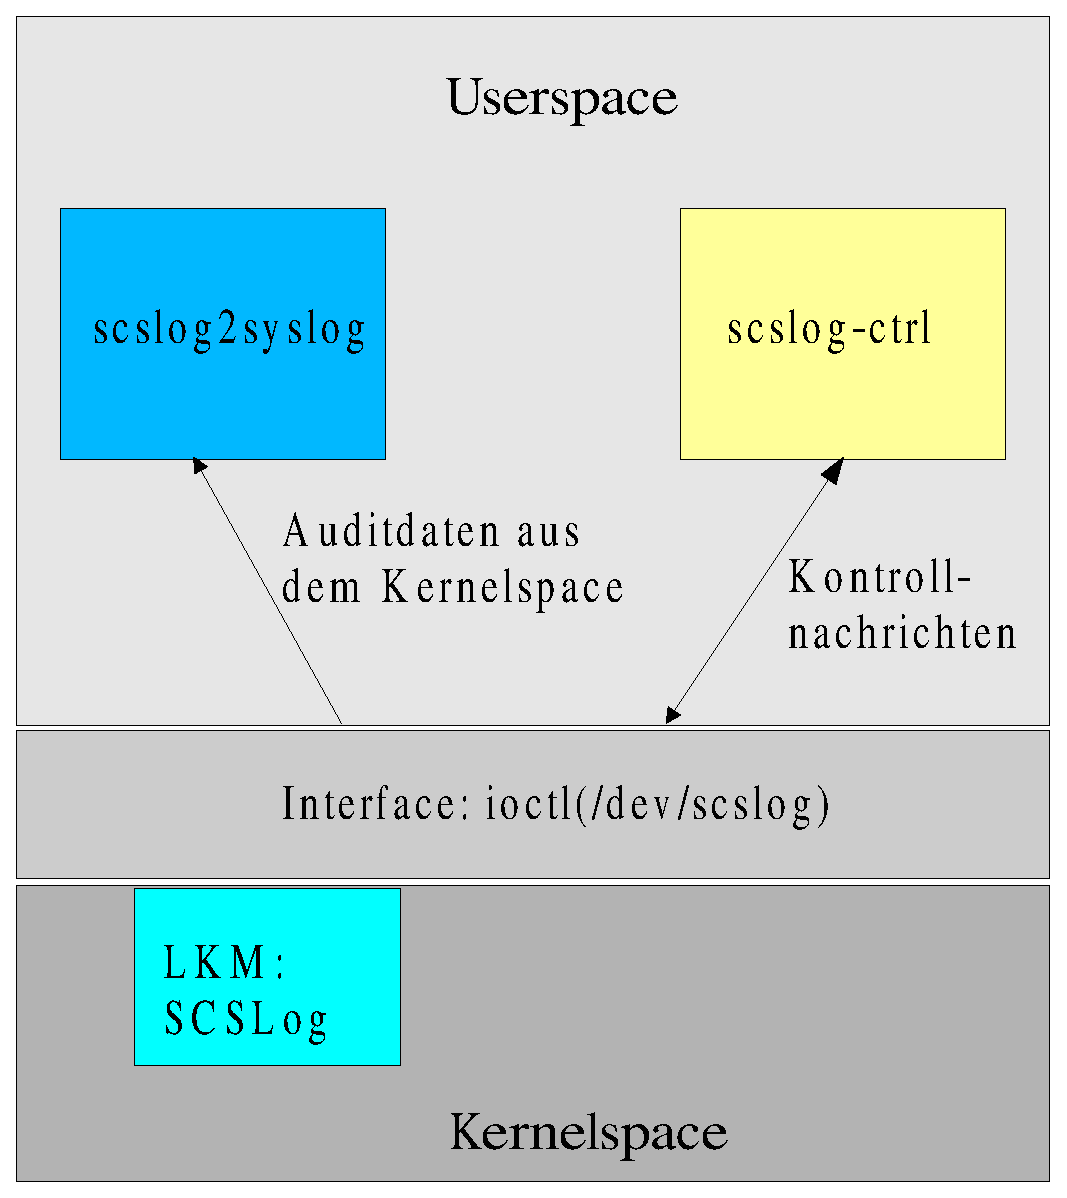
\includegraphics[scale=0.5]{SCSLog-Architektur.eps}
	\captionof{figure}{SCSLog Architektur}
\end{center}
\vspace{1cm}

\textit{SCSLog} besteht aus f"unf Teilen, drei LKMs und zwei Benutzerprogrammen:
\begin{itemize}
	\item scslog.o: Logging LKM
	\item scshide.o: versteckt ein LKM
	\item scsunrmv.o: macht ein LKM \glqq unentfernbar\grqq\/
	\item scslog--ctrl: Steuerung des SCSLog--Moduls
	\item scslog2syslog: Weiterleitung von SCSLog nach Syslog
\end{itemize}

\paragraph*{SCSLog} Das LKM \textit{SCSLog} muss die originalen, vom Kernel angebotenen, Systemaufrufe
durch seine Log--Funktionen erweitern. Die Systemaufrufe d"urfen nicht komplett ersetzt werden, da sonst
ein Arbeiten mit dem System nicht mehr m"oglich w"are. Um dies zu erreichen, wird die \textit{Syscall Table}
des Kernels ver"andert, indem der Zeiger auf die original Kernel--Funktion gesichert und anschlie"send
auf die Adresse der Log--Funktion gesetzt wird.

\begin{verbatim}
/* remember old value (pointer to original function) */
sci_table[syscall_num].bakup_ptr = sys_call_table[syscall_num];

[...]

/* replace with our funtion (intercept all calls) */
sys_call_table[syscall_num] = (void *) log_ptr;
\end{verbatim}
\vspace{1cm}
Folgende Funktion aus \textsf{scslog.o} "ubernimmt diese Aufgabe:
\begin{verbatim}
/*
** System Call-Table Redirect Routine
*/
static int redirect_syscall_table(u_int action,
                                  int syscall_num,
                                  char *syscall_name,
                                  int (*log_ptr)())
{

  DBG1(KERN_INFO "SCSLog - Debug: redirect_syscall_table...\n")

  switch(action)
  {
    case ACTION_WRAP:
      if(sci_table[syscall_num].logged == TRUE)
        return(-1);

      sci_table[syscall_num].logged = TRUE;

      printk(KERN_INFO "SCSLog - start monitoring syscall: %s()\n",
                                                                syscall_name);

      /* remember old value (pointer to original function) */
      sci_table[syscall_num].bakup_ptr = sys_call_table[syscall_num];

      /* replace with our funtion (intercept all calls) */
      sys_call_table[syscall_num] = (void *) log_ptr;
      break;
    case ACTION_UNWRAP:
      if(sci_table[syscall_num].logged != TRUE)
        return(-1);

      sci_table[syscall_num].logged = FALSE;

      printk(KERN_INFO "SCSLog - stop monitoring syscall: %s()\n"
                                                ,sci_table[syscall_num].name);

      /* restore old pointer */
      sys_call_table[syscall_num]       = sci_table[syscall_num].bakup_ptr;
      sci_table[syscall_num].bakup_ptr  = NULL;
      break;
    default:
      return(1);
  }

  return(0);
}
\end{verbatim}


Um die Analyse der Log--Daten von Benutzerapplikationen wie gefordert zu vereinfachen, wurde
ein einfaches Format gew"ahlt. Hier ein Beispiel (Zeile wurde umgebrochen):
\begin{verbatim}
Syscall: socketcall | Program: reactiondaemon | PID: 2083 |
UID: 0 | EUID: 0 | Call: 5 = socketcall(5, bffff414) |
Comment: accept from IP: 10.0.0.10 Port: 33211 |
\end{verbatim}

\pagebreak

Die Log--Zeile besteht aus sieben Elementen, die genug Informationen f"ur eine Analyse leifern
sollten.
\vspace{0.3cm}
\begin{center}
	\begin{tabular}{|c|l|l|}
	\hline
		\textbf{Feld}		& \textbf{Token}	& \textbf{Beschreibung}						\\ \hline
		1			& Syscall:		& Name des Syscalls					\\ \hline
		2			& Program:		& Programm, welches den Syscall ausf"uhrt		\\ \hline
		3			& PID:			& Prozess ID des Programms				\\ \hline
		4			& UID:			& reale User ID des Programms					\\ \hline
		5			& EUID:			& effektive User ID des Programms			\\ \hline
		6			& Call:			& kompletter Syscall mit R"uckgabewert und Paramentern	\\ \hline
		7			& Comment		& u.U. Kommentar zur weitern Erkl"arung			\\ \hline
	\end{tabular}
\end{center}
\vspace{1cm}

Der Linux--Kernel 2.4.18 bietet ca. 220 Syscalls an. Zum aktuellen Zeitpunkt werden aber nur die
wichtigsten Systemaufrufe unterst"utzt.
\begin{itemize}
	\item execve()
	\item chmod()
	\item open()
	\item symlink()
	\item setuid()
	\item setgid()
	\item setreuid()
	\item setregid()
	\item socketcall()
\end{itemize}

Im Konzept wurde festgelegt, einen Ringpuffer f"ur die Zwischenspeicherung zu benutzen. Nachfolgend
werden die globalen Variablen und Funktionen, die zur Handhabung des Ringpuffers notwendig sind, gezeigt.
\begin{verbatim}
/*
** Ring Buffer for buffering Log Data
*/
u_int rb_maxline = MAXBYTESPERLINE;
u_int rb_maxring = MAXLINESPERRING;

u_int rb_pos_w;
u_int rb_pos_r;
u_int rb_overflow_w;
u_int rb_overflow_r;
u_int rb_records;

char  ringbuffer[500][4096];

[...]

int   rb_write(char *log_data, int overwrite);
int   rb_read(char *log_data, int release);
[...]
\end{verbatim}

Zur Zeit ist dieser Ringpuffer noch statisch, es sind aber alle n"otigen Ans"atze im Quellcode
von \textit{SCSLog} vorhanden, um sp"ater die Gr"o"se aus der Benutzerebene via \texttt{ioctl(2)}
anpassen zu k"onnen.

\paragraph*{SCSHide} Um \textit{SCSLog} \glqq unsichtbar\grqq\/ werden zu lassen, wurde \textit{SCSHide} entwickelt,
welches sich eines einfachen Tricks bedient.
Der Linux--Kernel benutzt eine verkettete Liste, um Informationen "uber geladene LKMs zu verwalten. \textit{SCSHide}
geht nun diese Liste durch und sucht nach dem Modulnamen, den es als Argument auf der Befehlszeile erhalten
hat. Ist das Modul gefunden, wird der Zeiger aus dem vorigen Listenelement, der auf das zu versteckende Listenelement
zeigt, auf die Adresse f"ur das nachfolgende Element gesetzt. Somit ist der Eintrag f"ur unser Modul nicht
mehr Teil der Liste und somit unzug"anglich f"ur den Kernel.

Folgender Code ist daf"ur verantwortlich:
\begin{verbatim}
/* check the names of all modules loaded before scshide */
for(prevmod = thismod, currentmod = thismod->next;
      currentmod != NULL;
    prevmod = currentmod, currentmod = currentmod->next)
{
  if(strcmp(currentmod->name, module))
    continue;

  if(messages)
    printk(KERN_INFO "SCSHide - found module '%s'\n", currentmod->name);

  break;
}

if (currentmod == NULL)
{
  printk(KERN_INFO "SCSHide - module '%s' not found!\n", module);
  return(0);
}

/* remove the module structure from the modules list */
if(messages)
  printk(KERN_INFO "SCSHide - remove listentry of module '%s'\n",
                                                         currentmod->name);
prevmod->next = currentmod->next;
\end{verbatim}

\paragraph*{SCSUnrmv} Das LKM \textit{SCSUnrmv} ist das Letzte in der Reihe der Kernel--Module.
Genau wie \textit{SCSHide} ver"andert auch \textit{SCSUnrmv} die verkettete Liste im Linux--Kernel.
Dabei wird diesmal aber nicht die Reihenfolge der Liste ver"andert, sondern lediglich der \textit{Use Counter}
inkrementiert. Linux entfernt ein Modul nicht, solange der \textit{Use Counter} gr"o"ser als Null ist.

\paragraph*{SCSLog--Ctrl} Zur Steuerung des LKMs \textit{SCSLog} "uber die Ger"atedatei \textsf{/dev/scslog}
dient das Programm \textsf{scslog--ctrl}. So kann man bspw. wie folgt das Logging f"ur den Syscall
\texttt{open(2)} und \texttt{setuid(2)} ein-- und wieder ausschalten:

\begin{verbatim}
root@HotSpot# scslog-ctrl -s 5,23
root@HotSpot# scslog-ctrl -u 5,23
\end{verbatim}

Als kleines Beispiel soll gezeigt werden, wie "uber \texttt{ioctl(2)} das Logging f"ur einen beliebigen
Systemaufruf gesetzt wird, nachdem sicher gestellt wurde, dass dieser Systemaufruf nicht bereits "uberwacht
wird.
\begin{verbatim}
if((retval = ioctl(sdev, SCSLOG_IOCQLOGGING, &sc_table[idx].num)) < 0)
{
  err_mesg(WARN, "%s: Can't query status for syscall number %d (%s)"
               , pname, sc_table[idx].num, sc_table[idx].name);
  return(-2);
}

if(retval == TRUE)
  continue; // syscall already set, skip to the next

if(ioctl(sdev, SCSLOG_IOCSLOGGING, &sc_table[idx].num) < 0)
{
  err_mesg(WARN, "%s: Can't set monitoring for syscall number %d (%s)"
               , pname, sc_table[idx].num, sc_table[idx].name);
  return(-3);
}
\end{verbatim}


\paragraph*{Scslog2Syslog} Das Hilfsprogramm \textsf{scslog2syslog} hat lediglich die Aufgabe, in einer
Endlosschleife die Log--Zeilen von der Ger"atedatei \textsf{/dev/scslog} zu lesen und an \textit{Syslog} weiterzureichen.

\vspace{1cm}

\subsubsection{DataForwarder --- Datenweiterleitung}
Im Konzept wurde f"ur den \textit{DataForwarder} gefordert, dass die Privilegien des Super--Users
nur wenig genutzt werden und die logischen Teile, soweit wie m"oglich, in eigene Prozesse aufgeteilt
werden. Die untenstehende Abbildung zeigt das Design des \textit{DataForwarders}.
\vspace{1cm}
\begin{center}
	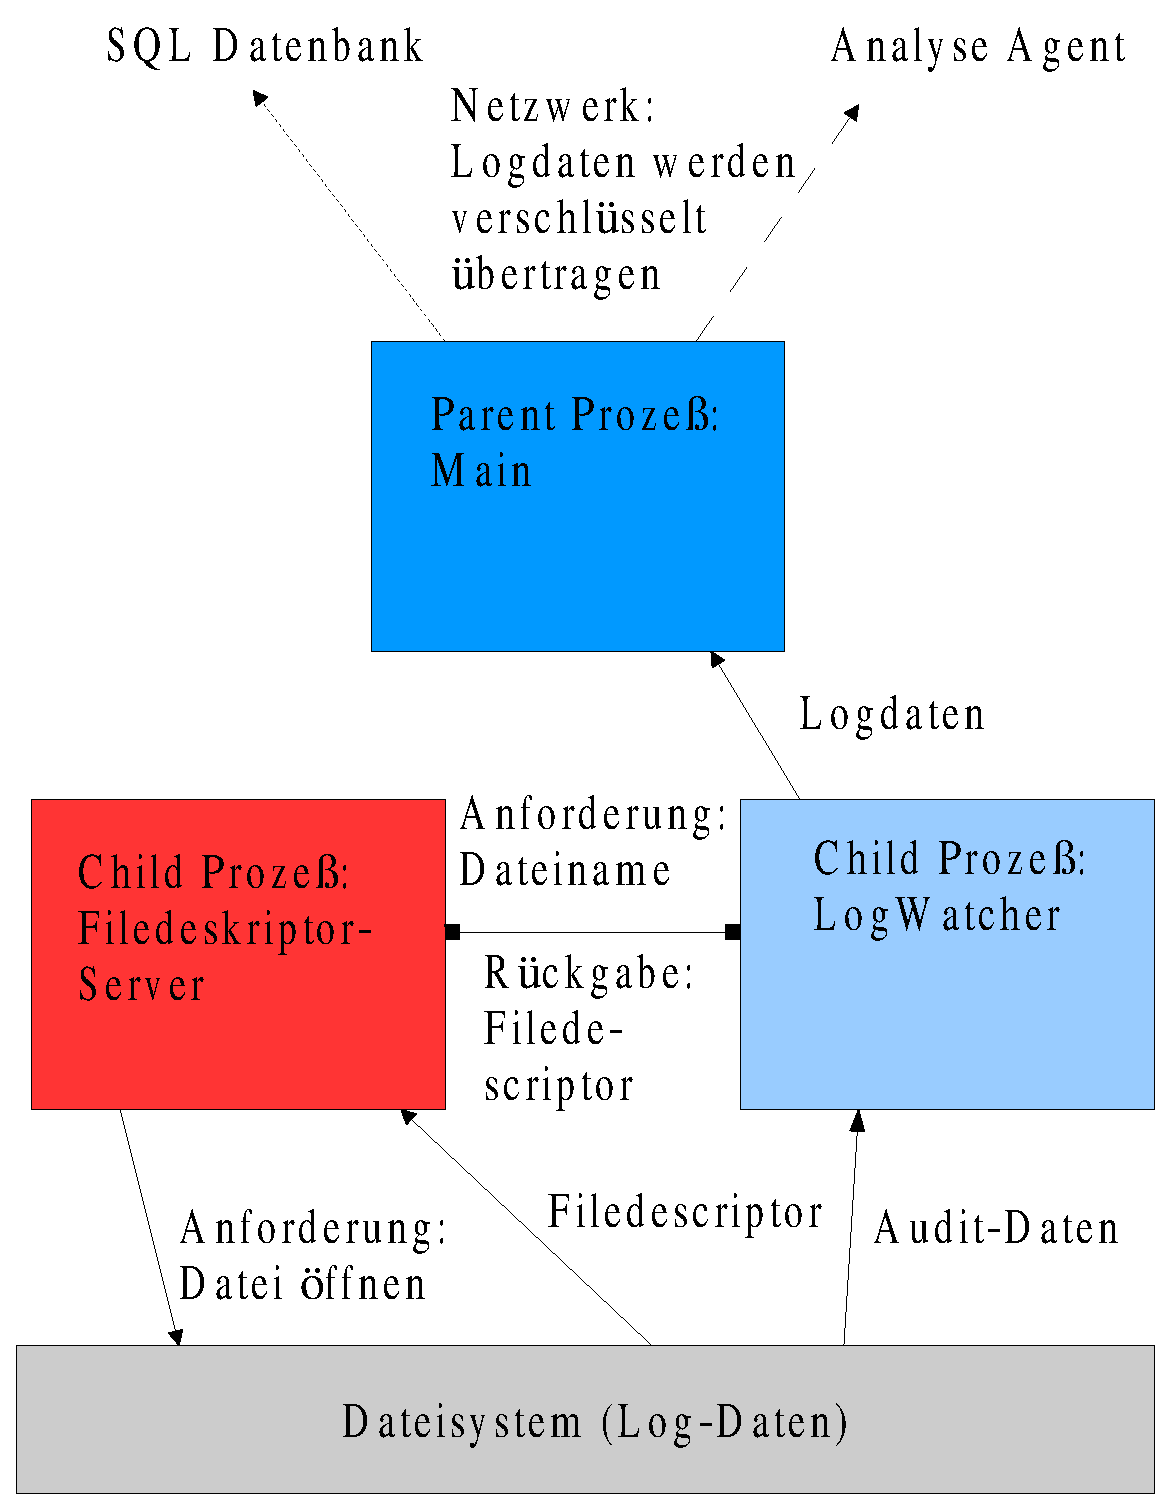
\includegraphics[scale=0.5]{Dataforwarder-Architektur.eps}
	\captionof{figure}{DataForwarder Architektur}
\end{center}
\vspace{1cm}

In diesem Modell l"auft nur der \textsf{Filedescriptor Server} (rot gekennzeichnet)
mit Super--User--Rechten, da er die zu "uberwachenden Dateien "offnet; die anderen beiden Prozesse
laufen mit normalen Benutzerrechten. Der \textsf{LogWatcher--Prozess} fordert den \textsf{Filedescriptor
Server} auf, eine bestimmte Datei zu "offnen und erh"alt dann den zugeh"origen Dateideskriptor
"uber einen \textit{Unix Domain Socket} zur"uck. Entdeckt der \textsf{LogWatcher--Prozess} neue Daten,
dann werden diese in einem \textit{Shared Memory Segment} geschrieben und dort f"ur die weitere Verarbeitung
vom \textsf{Main--Prozess} gelesen. Zur Synchronisation zwischen den beiden Prozessen f"ur Lese-- und
Schreibeoperationen von und in das \textit{Shared Memory Segment} dient ein \textit{Semaphore}.

\pagebreak

Desweiteren enthielt die Konzeptbeschreibung f"ur den \textit{DataForwarder} sechs Hauptaufgaben:
\begin{itemize}
	\item Sammlung
	\item Filterung
	\item Pseudonymisierung
	\item Formatierung
	\item Verschl"usselung
	\item Weiterleitung
\end{itemize}

%Die Namen und Pfade der Module f"ur Filterung, Pseudonymisierung und Formatierung der Log--Daten und
%deren Konfigurationsdatei werden aus der Datei \textsf{dataforwarder.conf} gelesen und mit \textsf{libtool}
%geladen.

\paragraph*{Sammlung} Aus der Konfigurationsdatei des \textit{DataForwarders} wird eine Liste
von Dateinamen gelesen, die durch den \textsf{Filedescriptor Server} ge"offnet und vom \textsf{LogWatcher}
"uberwacht werden. Der \textsf{LogWatcher} achtet dabei auf folgende Ver"anderung bei den Dateien:
\begin{itemize}
	\item Entfernung aus dem Dateisystem
	\item neuer Inode
	\item gestutzte Dateil"ange
	\item Modifikationszeit
\end{itemize}
Zus"atzlich ist die Reihenfolge, in der die Ver"anderungen gepr"uft werden, wichtig, da bspw. eine "Anderung
in der Modifikationszeit einer Datei nicht zwangsweise auf das Hinzuf"ugen von Daten schlie"sen l"asst.
Die Reihenfolge, wie sie oben in der Liste angegeben ist, ist auch die Reihenfolge, die im Code des
\textsf{LogWatchers} benutzt wird.

Bei der Bearbeitung der Dateien wird zwischen regul"aren Dateien und Ger"atedateien unterschieden. Bei Ger"atedateien
wird einfach gepr"uft, ob Daten zum Lesen vorhanden sind, wenn dem so ist, dann werden alle vorhandenen Daten
gelesen und in das \textit{Shared Memory Segment} geschrieben.

\paragraph*{Filterung} Die zur Filterung geforderten regul"aren Ausdr"ucke wurden mit Hilfe der
\glqq POSIX regex functions\grqq\/ der GNU C--Bibliothek implementiert. Das Filtermodul
\textsf{mice\_mod\_filter} wird im Kapitel \frqq Die Module\flqq\/ genauer betrachtet.

\paragraph*{Pseudonymisierung}
Das Pseudonymisierungsmodul \textsf{mice\_mod\_pseudonymizer} enth"alt keinen funktionalen Code.

\paragraph*{Formatierung} Die Formatierung wurde im Modul \textsf{mice\_mod\_logformat} implementiert
und wird ebenfalls im Kapitel \frqq Die Module\flqq\/ genauer beschrieben.

\paragraph*{Verschl"usselung} F"ur den kryptografischen Teil von \textsc{M--ICE} wurde die Bibliothek
MCrypt \cite{www-libmcrypt} benutzt.

\paragraph*{Weiterleitung} Die Konfigurationsdatei des \textit{DataForwarders} muss die IP--Adressen
und Port--Nummern vom Datenbank--Server und der Analyseeinheit enthalten, damit die Daten weitergeleitet
werden k"onnen. Sind IP--Adresse und Port--Nummer auf 0 gesetzt, wird nicht versucht, Daten an die
entsprechende Komponente zu schicken. Wenn eine Verbindung aufgrund eines Fehlers nicht zustande
kommen sollte, dann wird erneut versucht die Verbindung zu "offnen. Der untenstehende Code--Abschnitt
soll dies f"ur den SQL--Server verdeutlichen.
\begin{verbatim}
/*
** Send Data to MySQL Server.
*/
if(SqlSock >= 0)
{
  if(writen(SqlSock, (char *) &Message, sizeof(Message)) < 0)
  {
    log_mesg(WARN_SYS, "%s: Error while sending Data to SQL Server.
                        Try to reopen Connection...\n", cProgname);

    close(SqlSock);

    if((SqlSock = tcp_open(CfgSQLIP[iSectSQL], NULL, CfgSQLPort[iSectSQL])) < 0)
      log_mesg(WARN_SYS, "%s: Error while opening Socket to SQL Server.\n"
                       , cProgname);

    if(writen(SqlSock, (char *) &Message, sizeof(Message)) < 0)
    {
      log_mesg(WARN, "%s: Error while sending Data to SQL Server. Abort!\n"
                   , cProgname);
      close(SqlSock);
      exit(-1);
    }
  }
}
\end{verbatim}

%/*
%** Send Data to Analysis Unit
%*/
%if(AnaSock >= 0)
%{
%  if(writen(AnaSock, (char *) &Message, sizeof(Message)) < 0)
%  {
%    log_mesg(WARN_SYS, "%s: Error while sending Data to Analysis Server.
%                        Try to reopen Connection...\n", cProgname);
%
%    close(AnaSock);
%
%    if((AnaSock = tcp_open(CfgASIP[iSectAna], NULL, CfgASPort[iSectAna])) < 0)
%      log_mesg(WARN_SYS, "%s: Error while opening Socket to Analysis Server.\n"
%                       , cProgname);
%
%    if(writen(AnaSock, (char *) &Message, sizeof(Message)) < 0)
%    {
%      log_mesg(WARN, "%s: Error while sending Data to Analysis Server. Abort!\n"
%                   , cProgname);
%      close(AnaSock);
%      exit(-1);
%    }
%  }
%}

\vspace{1cm}
\begin{center}
	\includegraphics[scale=0.5]{DF-Datenfluss.eps}
	\captionof{figure}{Datenflussdiagramm des DataForwarders}
\end{center}
\vspace{1cm}


\subsubsection{BufferDaemon --- multifunktionaler Netzwerk--Server}
Der \textit{BufferDaemon} ist ein multifunktionaler Netzwerk--Server, der mit Hilfe von Modulen
verschiedene Datenformate (\textit{Encoding Modul\/}) vom Netz entgegennehmen und in bestimmten
Zeit-abst"anden
verarbeiten (\textit{Output Modul\/}) kann. Zur Zwischenspeicherung dient ein Ringpuffer, der entweder im
RAM oder "uber \textit{Memory Mapping\/} auf der Festplatte gehalten wird. Jede Zuordnung zwischen
\textit{Encoding Modul} und \textit{Output Modul} bekommt ihren eigenen Ringpuffer, ihren eigenen
Socket und einen eigenen Interval--Timer. Um diese Informationen zu verwalten, wird ein Array der
Struktur \texttt{ProcQ} benutzt.

\pagebreak

\begin{verbatim}
struct ProcessQueue
{
  struct ProcessQueue *prev;

  struct enc_info
  {
    int               iSock;
    saddr_in          SAddrIn;
    int               iCliSock;
    saddr_in          CliAddrIn;
    size_t            MsgSize;
    pthread_t         TID;
    char              *cModName;

    lt_dlhandle       dlHandle;
    const lt_dlinfo   *dlInfo;
    size_t            (*InitPtr)(char *);
    char *            (*FuncPtr)(char *, size_t);
    int               (*ClosePtr)(void);
  } Encoding;

  struct out_info
  {
    time_t            TimeInv;
    size_t            MsgSize;
    pthread_t         TID;
    char              *cModName;

    lt_dlhandle       dlHandle;
    const lt_dlinfo   *dlInfo;
    size_t            (*InitPtr)(char *);
    char *            (*FuncPtr)(char *, size_t);
    int               (*ClosePtr)(void);
  } Output;

  enum CacheMethod  CMethod;
  struct rb_info    Ringbuffer;
  struct mm_info    MMap;

  struct ProcessQueue *next;

} *ProcQ;
\end{verbatim}

Der \textit{BufferDaemon} lauscht an einem benutzerdefinierten Port, um Daten zu empfangen.
Die empfangenen Daten werden an das \textit{Encoding Modul} "ubergeben, dort dekodiert und
in Klartextform als eindimensionales Char--Array an den Aufrufer zur"uckgegeben.
Dieses Array wird im Ringpuffer gespeichert, nach einem bestimmten Zeitinterval vom
\textit{Output Modul} wieder ausgelesen und verarbeitet. Beide Module laufen
in verschiedenen Threads.
\begin{verbatim}
/*
** Call Encode-Modules Decode-Function to get Plaintext Message
*/
if
(
  (
    cDecodedMsg =
    (*ProcQ[ProcQEnt].Encoding.FuncPtr)(cEncodedMsg,
                                        ProcQ[ProcQEnt].Encoding.MsgSize)
  ) == NULL
)
{
  log_mesg(WARN, "%s: Error while decoding received Data!\n", cProgname);
  continue;
}

/*
** Now write the Plaintext Message to the Ringbuffer
*/
pthread_mutex_lock(&ProcQ[ProcQEnt].Ringbuffer.rb_mutex);
if
(
  intRBWrite(&ProcQ[ProcQEnt].Ringbuffer,
             cDecodedMsg, ProcQ[ProcQEnt].Output.MsgSize,
             TRUE) < 0
)
{
  log_mesg(WARN, "%s: Error: intRBWrite(cDecodedMsg,
                  ProcQ[ProcQEnt].Output.MsgSize, TRUE)!\n", cProgname);
}

pthread_mutex_unlock(&ProcQ[ProcQEnt].Ringbuffer.rb_mutex);

[...]

/*
** Read Data from Ringbuffer
*/
pthread_mutex_lock(&ProcQ[ProcQEntry].Ringbuffer.rb_mutex);
while
(
  intRBRead(&ProcQ[ProcQEntry].Ringbuffer,
            cMsg,
            ProcQ[ProcQEntry].Output.MsgSize,
            TRUE) != -1
)
{
  /*
  ** Call Module Function
  */
  if
  (
    (*ProcQ[ProcQEntry].Output.FuncPtr)(cMsg,ProcQ[ProcQEntry].Output.MsgSize)
    < 0
  )
  {
    log_mesg(WARN, "%s: Debug: Error while calling Modules FUNC Function\n"
                 , cProgname);
  }

  memset(cMsg, 0, ProcQ[ProcQEntry].Output.MsgSize);
}
pthread_mutex_unlock(&ProcQ[ProcQEntry].Ringbuffer.rb_mutex);
\end{verbatim}

\vspace{1cm}
\begin{center}
	\includegraphics[scale=0.5]{BD-Datenfluss.eps}
	\captionof{figure}{Datenflussdiagramm des BufferDaemons}
\end{center}
\vspace{1cm}


\subsubsection{ReactionProcess --- Reaktionen nach Ma"s}
Die \textit{ReactionProcesses} lesen die \textit{Reaction Message\/}, die vom Management--Host
geschickt wurde,  von einem FIFO und f"uhren Ihre Aktion aus. \textsc{M--ICE} ist
bei der Menge und Art seiner Reaktionen sehr flexibel, d.h. es kann jede denkbare Reaktion
implementiert werden.

Aufbau der \textit{Reaction Message\/}:
\begin{verbatim}
typedef struct
{
  char    cIdmefMsg[MAX_IDMEFMSGSIZE+1]          __attribute__ ((packed));
  char    cAlertID[RIDMSG_MAX_ALERTID+1]         __attribute__ ((packed));
  char    cAlertIDDesc[RIDMSG_MAX_ALERTDESC+1]   __attribute__ ((packed));
  int     iRID;
} RIDMsgFormat;
\end{verbatim}
\vspace{1cm}

Folgende Reaktionsm"oglichkeiten wurden implementiert.
\begin{center}
	\begin{tabular}{|c|c|}
		\hline
		\textbf{Name}			& \textbf{Beschreibung}						\\ \hline
		rid\_1\_write\_to\_syslog	& Gibt Alarminformationen an Syslog weiter			\\ \hline
		rid\_2\_send\_to\_alert\_db	& Schickt Alarminformationen zur Speicherung an eine Datenbank	\\ \hline
		rid\_3\_save\_to\_file		& Schreibt die rohe IDMEF--Message in eine Datei			\\ \hline
		rid\_4\_countermeasure		& Informiert den ReactionDaemon "uber Gegenma"snahmen		\\ \hline
	\end{tabular}
\end{center}
\vspace{1cm}

\begin{center}
	\includegraphics[scale=0.5]{RP-Datenfluss.eps}
	\captionof{figure}{Datenflussdiagramm des ReactionProcess'}
\end{center}
\vspace{1cm}


\subsubsection{ReactionDaemon --- Reaktionen ausf"uhren}
F"ur den \textit{ReactionDaemon} wird eine Art \textit{Remote Procedure Call\/} ben"otigt.
Die angebotenen Funktionen werden hier ebenfalls als Module eingebunden.
Unser Protokoll erlaubt jeweils drei Modi f"ur Client-- und f"ur Server--Nachrichten.

Client--Nachrichten:
\begin{center}
	\begin{tabular}{|c|c|}
		\hline
		\textbf{Modus}	& \textbf{Beschreibung}			\\ \hline
		EXEC		& F"uhre Funktion aus			\\ \hline
		SHOW		& Zeige alle angebotenen Funktionen an	\\ \hline
		CHECK		& "Uberpr"ufe ob Funktion unterst"utzt	\\ \hline
	\end{tabular}
\end{center}

Server--Nachrichten:
\begin{center}
	\begin{tabular}{|c|c|}
		\hline
		\textbf{Modus}	& \textbf{Beschreibung}				\\ \hline
		RETVAL		& R"uckgabewert der ausgef"uhrten Funktion	\\ \hline
		ALL		& R"uckgabe aller angebotenen Funktionen	\\ \hline
		SUPPORTED	& Funktion wird unterst"utzt			\\ \hline
	\end{tabular}
\end{center}

\vspace{1cm}

Die Strukturen f"ur den \textit{Remote Procedure Call\/} werden nachfolgend gezeigt,
dabei ist f"ur die einzelnen Modi jeweils eine Struktur vorhanden, diese Struktur
wird dann in die eigentliche \textit{Reaction Message}--Struktur eingef"ugt.
\begin{verbatim}
typedef struct
{
  char      alert_id[RIDMSG_MAX_ALERTID+1];
  u_int     reaction_id;
  uid_t     uid_for_exec;
  gid_t     gid_for_exec;
  u_int     function_id;
  u_int     num_of_args;
  char      arg_fmt_string[MAX_ARGSTRG_SIZE+1]  __attribute__ ((packed));
  char      arg_fmt_param[MAX_FMTSTRG_SIZE+1]   __attribute__ ((packed));
} stExecMsg;

typedef struct
{
  u_int     show;
} stShowMsg;

typedef struct
{
  u_int     function_id;
} stCheckMsg;

typedef struct
{
  int     ret_val;
} stRetvalMsg;

typedef struct
{
  struct
  {
    u_int   uiID;
    char    *cModName[MAX_MODNAME+1]  __attribute__ ((packed));
  } Function[MAX_FUNCID]              __attribute__ ((packed));
} stAllMsg;

typedef struct
{
  u_int     supported;
} stSupportedMsg;


typedef struct
{
  short     sChkSum;
  time_t    Timestamp;

  u_int     Mode;

  union
  {
    stExecMsg       Exec;
    stShowMsg       Show;
    stCheckMsg      Check;
    stRetvalMsg     Retval;
    stAllMsg        All;
    stSupportedMsg  Supported;
  } ModeData;

} stReactionMsg;
\end{verbatim}

\pagebreak

Die auszuf"uhrende Funktion im EXEC--Modus wird "uber eine \textsf{Function ID} Nummer bestimmt.
Die \textsf{Function ID} ist direkt einem Modul zugeordnet. Die Konfigurationsdatei des
\textit{ReactionDaemons} verdeutlicht dies gut:
\begin{verbatim}
[FUNCTION_ID]
FID = 0x000001

[REACTION_MODULES]
RCT_MOD = mice_mod_rct_system

[REACTION_MODULES_CONFIG_FILE]
RCT_FILE = /etc/M-ICE/mice_mod_rct_system.conf
\end{verbatim}

\vspace{1cm}
\begin{center}
	\includegraphics[scale=0.5]{RD-Datenfluss.eps}
	\captionof{figure}{Datenflussdiagramm des ReactionDaemons}
\end{center}
\vspace{1cm}


\subsection{Die Module}
Wie zuvor schon erw"ahnt, wurden wichtige Funktionen in dynamisch ladbare Module ausgelagert, um
die Flexibilit"at und Erweiterbarkeit weiter zu erh"ohen.
Im Laufe der Entwicklung von \textsc{M--ICE} wurden einige Module implementiert,
die hier nur kurz erkl"art werden sollen.

\pagebreak

Die meisten Module bestehen lediglich aus einer Konfigurationsdatei und dem Modul selbst:
\begin{itemize}
	\item /etc/M-ICE/mice\_mod\_$<$name$>$.conf
	\item /lib/M-ICE/mice\_mod\_$<$name$>$.*
\end{itemize}

\vspace{0.5cm}

Jedes Modul muss drei Funktionen zur Verf"ugung stellen:
\begin{itemize}
	\item mice\_mod\_$<$name$>$\_LXT\_init: Initialisierung des Moduls
	\item mice\_mod\_$<$name$>$\_LXT\_func: eigentliche Funktion
	\item mice\_mod\_$<$name$>$\_LXT\_close: Modul schlie"sen
\end{itemize}

\vspace{0.5cm}

Die Funktionen haben folgende Argumente:
\begin{center}
	\begin{tabular}{|c|c|}
		\hline
		\textbf{Funktion}	& \textbf{Argumente}			\\ \hline
		init			& \texttt{char *cConfigFile}			\\ \hline
		func			& funktionsabh"angig			\\ \hline
		close			& \texttt{void}					\\ \hline
	\end{tabular}
\end{center}

\vspace{0.5cm}

\subsubsection{mice\_mod\_filter}
Zur Datenreduktion wird direkt auf dem Client mit Hilfe von regul"aren Ausdr"ucken gefiltert.
Die Filterregeln werden einfach in die Konfigurationsdatei \textsf{mice\_mod\_filter.conf}
eingetragen und durch folgenden Code verarbeitet:

\begin{verbatim}
for
(
  TmpList = _mmf_CfgRules[_mmf_iSectFilterRules];
    TmpList != NULL;
  TmpList = TmpList->next
)
{
  if(re_compile_pattern(TmpList->str, strlen(TmpList->str), _mmf_RegExBuf) != 0 )
  {
    log_mesg(WARN, "mice_mod_filter: Error while compiling Regular Expression
                    '%s'. Skipped...\n", TmpList->str);
    continue;
  }

  _mmf_RegExBuf->regs_allocated = REGS_FIXED;

  if(re_match(_mmf_RegExBuf, cLogData, LogDataLen, 0, NULL) >= 0)
    break;
}

if(TmpList != NULL)
{
  /*
  ** We find a matching Pattern.
  ** Let's skip this Logentry, because the User wants to filter it out.
  */
  return(1);
}

return(0);
\end{verbatim}
Das Filtermodul gibt 1 an den Aufrufer zur"uck, wenn die Regel zutrifft, und 0 wenn nicht.
Dem Aufrufer ist nun "uberlassen, was er mit dieser Information anf"angt. In unserem Fall
ignorieren wir bei einem R"uckgabewert von 1 den Log--Eintrag.

\vspace{0.5cm}

\subsubsection{mice\_mod\_logformat}
Um die nativen Log--Daten des Clients mit weiteren wichtigen Informationen anzureichern,
benutzt der \textit{DataForwarder} das Modul \textsf{mice\_mod\_logformat}.
%\vspace{0.5cm}
Die Struktur der aufgewerteten Audit--Daten sieht wie folgt aus:
\begin{verbatim}
typedef struct
{
  char    cHost     [MAX_HOST]      __attribute__ ((packed));
  char    cDomain   [MAX_DOMAIN]    __attribute__ ((packed));
  char    cIP       [MAX_IP]        __attribute__ ((packed));
  char    cOSystem  [MAX_OS]        __attribute__ ((packed));
  char    cRelease  [MAX_RELEASE]   __attribute__ ((packed));
  char    cVersion  [MAX_VERSION]   __attribute__ ((packed));
  char    cDate     [MAX_DATE]      __attribute__ ((packed));
  char    cTime     [MAX_TIME]      __attribute__ ((packed));
  char    cLogLine  [MAX_DATA]      __attribute__ ((packed));
  u_short sChkSum                   __attribute__ ((packed));
} LogFormat;
\end{verbatim}

\vspace{0.5cm}

\subsubsection{mice\_mod\_pseudonymizer}
Ein Pseudonymisierungsverfahren wurde nicht implementiert.

\vspace{0.5cm}

\subsubsection{mice\_mod\_mysql}
Damit der \textit{BufferDaemon} die Audit--Daten in eine MySQL--Datenbank speichern kann, l"adt er
das Modul \textsf{mice\_mod\_mysql} als \textit{Output Modul}. Dieses Modul verwaltet drei Tabellen
\texttt{rawlog\_line}, \texttt{scslog\_line} und \texttt{firewall\_line}.
Die \textit{SCSLog}-- und die \textit{SuSEfirewall2}--Eintr"age werden vom Modul analysiert,
dabei werden die Daten in die entsprechenden Tokens und deren Werte aufgespalten. Die Werte werden
in die dazugeh"orige Spalte der jeweiligen Tabelle eingetragen. Diese Aufteilung erm"oglicht es dem
Anwender zielgenau nach Systemaufrufen, Benutzeridentit"aten, IP--Adressen, Port--Nummern und dergleichen
zu suchen.

\vspace{0.5cm}

Tabellenaufbau f"ur \textit{Syslog}:
\begin{verbatim}
CREATE TABLE rawlog_line  ( hostname    TEXT,
                            domain      TEXT,
                            ip          TEXT,
                            osystem     TEXT,
                            release     TEXT,
                            version     TEXT,
                            date        DATE,
                            time        TIME,
                            logline     TEXT,
                            signature   TEXT );
\end{verbatim}

Tabellenaufbau f"ur \textit{SCSLog}:
\begin{verbatim}
CREATE TABLE scslog_line  ( hostname    TEXT,
                            domain      TEXT,
                            ip          TEXT,
                            osystem     TEXT,
                            release     TEXT,
                            version     TEXT,
                            date        DATE,
                            time        TIME,
                            syscall     TEXT,
                            program     TEXT,
                            pid         INT     UNSIGNED  NOT NULL,
                            uid         INT     UNSIGNED  NOT NULL,
                            euid        INT     UNSIGNED  NOT NULL,
                            call        TEXT,
                            comment     TEXT );
\end{verbatim}

\pagebreak

Tabellenaufbau f"ur \textit{SuSEfirewall2}:
\begin{verbatim}
CREATE TABLE firewall_line  ( action      TEXT,
                              if_in       TEXT,
                              if_out      TEXT,
                              mac         TEXT,
                              source      TEXT,
                              destination TEXT,
                              ip_length   TEXT,
                              tos         TEXT,
                              prec        TEXT,
                              ttl         TEXT,
                              id          TEXT,
                              protocol    TEXT,
                              src_port    TEXT,
                              dst_port    TEXT,
                              pac_length  TEXT,
                              date        DATE,
                              time        TIME );
\end{verbatim}

\vspace{0.5cm}

\subsubsection{mice\_mod\_aa\_regex}
Das Analysemodul verarbeitet die Log--Daten aus dem Ringpuffer des \textit{BufferDaemons} mit Hilfe
von regul"aren Ausdr"ucken. Dabei werden nach erfolgreicher Erkennung intern Informationen "uber die
passende Regel gespeichert. Hier ein Beispiel f"ur die \texttt{Authentication Messages}:
\begin{verbatim}
/******************************************************************************
**
** A U T H   R U L E S
**
******************************************************************************/

// Auth Success
for(TmpList = _mice_mod_aa_regex_CfgAuth.aCfgAuthSucc
              [_mice_mod_aa_regex_CfgAuth.iSectionNr],
    iRuleCtr = 0;
      TmpList != NULL;
    TmpList = TmpList->next, iRuleCtr++)
{
  if(_mice_mod_aa_regex_DoesMatch(cLogLine, LogLineLen, TmpList->str) == TRUE)
  {
    /*
    ** Fill in Match Info Data
    */
    mInfo->iMatched     = TRUE;
    mInfo->iSectNr      = _mice_mod_aa_regex_CfgAuth.iSectionNr;
    mInfo->iSectType    = ST_AUTH;
    mInfo->iRuleNr      = iRuleCtr;
    mInfo->cRuleType    = RT_AUTH_S;
    mInfo->cMatchedRule = TmpList->str;
    mInfo->cSendTo      = _mice_mod_aa_regex_CfgAuth.cCfgSendTo
                          [_mice_mod_aa_regex_CfgAuth.iSectionNr];

    return(TRUE);
  }
}
\end{verbatim}

\vspace{0.5cm}

Die Informationen werden sp"ater ben"otigt, um unsere IDMEF--Nachricht zu bauen. Daf"ur werden folgende
Funktionen von \textsf{mice\_mod\_aa\_regex} benutzt:
\begin{itemize}
	\item \texttt{xmlNodePtr \_mice\_mod\_aa\_regex\_FormatIDMEF(LogFormat LogFmt, MatchInfo mInfo)}
	\item \texttt{xmlNodePtr \_mice\_mod\_aa\_regex\_BuildMsg(LogFormat LogFmt, MatchInfo mInfo)}
	\item \texttt{xmlNodePtr \_mice\_mod\_aa\_regex\_BuildMsgTree(LogFormat LogFmt, MatchInfo mInfo)}
	\item \texttt{xmlNodePtr \_mice\_mod\_aa\_regex\_BuildAnalyzer(LogFormat LogFmt)}
	\item \texttt{xmlNodePtr \_mice\_mod\_aa\_regex\_BuildSource(LogFormat LogFmt)}
	\item \texttt{xmlNodePtr \_mice\_mod\_aa\_regex\_BuildTarget(LogFormat LogFmt)}
\end{itemize}

\vspace{0.5cm}

In der Funktion \texttt{\_mice\_mod\_aa\_regex\_BuildMsgTree\/} werde alle IDMEF--Klassen zusammengef"uhrt:
\begin{verbatim}
MessageClass  = newIDMEF_Message
                (
                  newAttribute("version",IDMEF_MESSAGE_VERSION),
                  newAlert
                  (
                    newSimpleElement("ident",
                       intToString(_mice_mod_aa_regex_StaticInfo.ulAlertID)),
                    AnalyzerClass,
                    newCreateTime(NULL),
                    newDetectTime(NULL),
                    newAnalyzerTime(NULL),
                    SourceClass,
                    TargetClass,
                    newClassification
                    (
                      newAttribute("origin", "vendor-specific"),
                      newSimpleElement("name", mInfo.cRuleType),
                      newSimpleElement("url", "http://unkonwn.de"),
                      NULL
                    ),
                    newAdditionalData
                    (
                      newAttribute("meaning","Logline"),
                      newAttribute("type","string"),
                      newSimpleElement("value", LogFmt.cLogLine),
                      NULL
                    ),
                    NULL
                  ),
                  NULL
                );
\end{verbatim}

\vspace{0.5cm}

Nachdem die IDMEF--Nachricht gebaut wurde, wird sie mit dem Twofish--Algorithmus verschl"usselt und
an ihr Ziel geschickt.
Als Ziel kann nichts, der Management--Host, die Analyseeinheit oder beide angegeben werden.
Dieses Verhalten kann f"ur jede Kategorie in der Konfigurationsdatei des Analysemoduls seperat
gesetzt werden. Es ist denkbar, bereits analysierte Daten mit Hilfe eines anderen Verfahrens
von einem anderen Analyseagenten genauer untersuchen zu lassen oder Statistiken zu f"uhren.

\vspace{0.5cm}

\subsubsection{mice\_mod\_enc\_logformat\_twofish}
Zum Lesen der Daten vom \textit{DataForwarder} muss der \textit{BufferDaemon} das \textit{Encoding Modul}
\textsf{mice\_mod\_enc\_logformat\_twofish} laden.

\begin{verbatim}
memcpy(cDecodedMsg, CMsg->cCipherText, CMsg->CipherTextLen);

for(iCnt = 0; iCnt < CMsg->CipherTextLen; iCnt++)
  mdecrypt_generic(_mice_mod_enc_logformat_twofish_CryptoInfo.CryptModule,
                   &cDecodedMsg[iCnt], 1);

LFmt = (LogFormat *) cDecodedMsg;

[...]

/*
** Verify Checksum (CRC)
*/
sChkSum_Orig    = LFmt->sChkSum;
LFmt->sChkSum   = 0;
sChkSum_New     = in_chksum((u_short *) LFmt, sizeof(LogFormat));

if(sChkSum_Orig != sChkSum_New)
{
  log_mesg(WARN, "%s: Debug: Checksum does not match... skipping Message\n",
  _mice_mod_enc_logformat_twofish_cProgname);
  free(cDecodedMsg);
  return(NULL);
}

LFmt->sChkSum = sChkSum_Orig;

return(cDecodedMsg);
\end{verbatim}

\vspace{0.2cm}

\subsubsection{mice\_mod\_enc\_idmef\_twofish}
Der \textit{BufferDaemon}, der auf dem Management--Host l"auft, liest das IDMEF--Format der
Analyseeinheit mit Hilfe des \textit{Encoding Moduls} \textsf{mice\_mod\_enc\_idmef\_twofish}.
Dieses Modul unterscheidet sich strukturell nicht besonders vom Modul
\textsf{mice\_mod\_enc\_logformat\_twofish}. Es wird nach der Validierung der Pr"ufsumme
lediglich ein Zeiger auf eine IDMEF--Nachricht zur"uckgegeben und nicht auf eine
\textsf{LogFormat}--Nachricht.

\vspace{0.5cm}

\subsubsection{mice\_mod\_act\_generic}
Das Modul \textsf{mice\_mod\_act\_generic} dient als \textit{Output Modul} f"ur den \textit{BufferDaemon},
um auf dem Management--Host die Forderungen nach ausbaubaren und system"ubergreifenden
Reaktionen zu erf"ullen. Der Schl"ussel f"ur diese Eigenschaft ist das sog. \textit{Match File}.
Die \textsf{Analyzer ID\/}, die in der IDMEF--Nachricht kodiert ist, wird
dazu benutzt, um das richtige \textit{Match File\/} ausfindig zu machen. Die richtige Zuordnung wird
durch folgende Schleifenverschachtelung eruiert:

\begin{verbatim}
for(iCnt_Matchfile = 0; iCnt_Matchfile <= MFInfoEntries; iCnt_Matchfile++)
{
  for(iCnt_Alert = 0; iCnt_Alert < IDMEFmsg->nalerts; iCnt_Alert++)
  {
    for
    (
      iCnt_Classification = 0;
        iCnt_Classification < IDMEFmsg->alerts[iCnt_Alert]->nclassifications;
      iCnt_Classification++
    )
    {
      // Check for RID 1
      for(iCnt_AID = 0;
            iCnt_AID <= stMFInfo[iCnt_Matchfile].AID_1Entries;
          iCnt_AID++)
      {
        if(stMFInfo[iCnt_Matchfile].iAID_1[iCnt_AID] == -1) // no entry
          continue;

        // Should we react on this AlertID?
        if
        (
          !strcasecmp(IDMEFmsg->alerts[iCnt_Alert]->
                                classifications[iCnt_Classification]->
                                name,
                      stMFInfo[iCnt_Matchfile].
                      sAIDValList[stMFInfo[iCnt_Matchfile].
                      iAID_1[iCnt_AID]])
        )
        {
          _mice_mod_act_generic_ProcessReaction
          (
            cData,
            RID_1,
            stMFInfo[iCnt_Matchfile].
            sAIDValList[stMFInfo[iCnt_Matchfile].
            iAID_1[iCnt_AID]],
            stMFInfo[iCnt_Matchfile].
            sAIDDescList[stMFInfo[iCnt_Matchfile].
            iAID_1[iCnt_AID]]
          );
        }
      }
      [...]
    }
  }
}
\end{verbatim}
In diesem Codest"uck sieht man, wie jede Klassifikation, aller Alarme aus der IDMEF-Nachricht
mit dem Inhalt jedes \textit{Match Files} verglichen wird, um eine m"ogliche Reaktion zu finden.


\vspace{0.5cm}

\subsubsection{mice\_mod\_rct\_system}
Dieses Modul ist das letzte in einer langen Kette von Knotenpunkten in \textsc{M--ICE}'s Datenverarbeitung.
Der \textit{ReactionDaemon} auf dem Client benutzt dieses
Modul, um f"ur die dazugeh"orige \texttt{Function ID} eine Aktion auf dem Client zu veranlassen.
Das Modul \textsf{mice\_mod\_rct\_system} ruft einfach \texttt{system(3)} auf, um einen Befehl
auf Shellebene auszuf"uhren. Die \texttt{Function ID} und der dazugeh"orige Befehl stammen
vom \textit{Countermeasure Reaction Process} des Management--Hosts.
Die Implementierung von \textsf{mice\_mod\_rct\_system} soll nur als Beispiel dienen, um die
Funktionalit"at von \textsc{M--ICE} voll zu testen.
% und den Kreis von Aktion auf dem Client zu Reaktion auf dem Client zu schlie"sen.


\subsection{Die kryptografischen Protokolle}
Bei der Datenverschl"usselung wurden drei Ziele verfolgt:
\begin{itemize}
	\item Schutz vor Manipulation
	\item Schutz vor unbefugtem Lesen
	\item Schutz gegen \textit{Replay Attacken\/}
\end{itemize}

\paragraph*{Schutz vor unbefugtem Lesen und Manipulation}
Die geforderte Pr"ufsumme von unserem Klartext wird vom Sender berechnet und
vom Empf"anger nach der Entschl"usselung "uberpr"uft. Als erkl"arendes Beispiel soll hier die
\textit{LogFormat}--Nachricht zwischen \textit{DataForwarder} und \textit{BufferDaemon} der
Analyseeinheit dienen:
\begin{verbatim}
typedef struct
{
  char    cHost     [MAX_HOST]      __attribute__ ((packed));
  char    cDomain   [MAX_DOMAIN]    __attribute__ ((packed));
  char    cIP       [MAX_IP]        __attribute__ ((packed));
  char    cOSystem  [MAX_OS]        __attribute__ ((packed));
  char    cRelease  [MAX_RELEASE]   __attribute__ ((packed));
  char    cVersion  [MAX_VERSION]   __attribute__ ((packed));
  char    cDate     [MAX_DATE]      __attribute__ ((packed));
  char    cTime     [MAX_TIME]      __attribute__ ((packed));
  char    cLogLine  [MAX_DATA]      __attribute__ ((packed));
  u_short sChkSum                   __attribute__ ((packed));
} LogFormat;

typedef struct
{
  u_int       IVLen                               __attribute__ ((packed));
  char        IV[16]                              __attribute__ ((packed));
  u_int       CipherTextLen                       __attribute__ ((packed));
  char        cCipherText[1*sizeof(LogFormat)]    __attribute__ ((packed));
} CipherMsg;
\end{verbatim}

\vspace{1cm}

In \texttt{LogFormat.sChkSum} wird die Pr"ufsumme unserer \texttt{LogFormat}--Klartextnachricht
gespeichert. Anschlie"send wird die \texttt{LogFormat}--Struktur mit
Hilfe des Twofish--Algorithmus verschl"usselt und nach \texttt{cCipherText[]} kopiert.
Um Entwicklungs- und Ausf"uhrungszeit zu sparen wurde zur Berechnung der Pr"ufsumme ein
einfacher \textit{Cyclic Redundant Check}--Algorithmus und kein krypthografisch sicherer
Hashalgorithmus, wie bspw. SHA, benutzt. Das Erstellen der Pr"ufsumme geschieht im Modul \textsf{mice\_mod\_logformat}:
\begin{verbatim}
/*
** Keep Data Integrity by calculating a CRC sum
*/
LogEntry->sChkSum = 0;
LogEntry->sChkSum = in_chksum((u_short *) LogEntry, sizeof(LogFormat));
\end{verbatim}

\vspace{1cm}

Die \texttt{Chipher Message}, die unsere verschl"usselte \texttt{LogFormat}--Struktur als Nutzlast
enth"alt, wird nun von dem \textit{DataForwarder\/} "uber ein Netzwerk an einen Server geschickt.
\begin{verbatim}
for(iCnt = 0; iCnt < sizeof(LogFormat); iCnt++)
  mcrypt_generic(CryptModule, &Message.cCipherText[iCnt], 1);

[...]

if(writen(SqlSock, (char *) &Message, sizeof(Message)) < 0)
{
  log_mesg(WARN_SYS, "%s: Error while sending Data to SQL Server.
                          Try to reopen Connection...\n", cProgname);

[...]
\end{verbatim}

\vspace{1cm}

Der \textit{BufferDaemon} muss dann nur noch die empfangene Nachricht entschl"usseln, die
Pr"ufsumme berechnen und mit der vom Client mitgeschickten Pr"ufsumme vergleichen.
Dieser Prozess findet im \textit{Encoding Modul\/} statt, bspw. in
\textsf{mice\_mod\_enc\_logformat\_twofish}.
\begin{verbatim}
/*
** Message is encryted. Let's decrypt it!
*/
[...]
memcpy(cDecodedMsg, CMsg->cCipherText, CMsg->CipherTextLen);

for(iCnt = 0; iCnt < CMsg->CipherTextLen; iCnt++)
  mdecrypt_generic(_mice_mod_enc_logformat_twofish_CryptoInfo.CryptModule,
                   &cDecodedMsg[iCnt], 1);

LFmt = (LogFormat *) cDecodedMsg;

/*
** Verify Checksum (CRC)
*/
sChkSum_Orig    = LFmt->sChkSum;
LFmt->sChkSum   = 0;
sChkSum_New     = in_chksum((u_short *) LFmt, sizeof(LogFormat));

if(sChkSum_Orig != sChkSum_New)
{
  log_mesg(WARN, "%s: Debug: Checksum does not match... skipping Message\n"
               , _mice_mod_enc_logformat_twofish_cProgname);
  free(cDecodedMsg);
  return(NULL);
}

LFmt->sChkSum = sChkSum_Orig;
\end{verbatim}

\vspace{0.5cm}

\paragraph*{Replay Attacken} Der Schutz vor \textit{Replay Attacken}, wie sie im Kapitel \frqq Konzepte\flqq\/
beschrieben wurden, wurde wie folgt umgesetzt:

\begin{verbatim}
/*
** Handle Client Request - Thread
*/
void  *voidHandleClientRequest(void *vArg)
{
  [...]

  time_t CurrentTimestamp = time(NULL) - REPLAYATTACK_DELAYWINDOW;

  [...]

  /*
  ** Check Timestamp to avoid replay attacks
  */
  if((time_t) ntohl(RctMsgPtr->Timestamp) > CurrentTimestamp)
    CurrentTimestamp = (time_t) ntohl(RctMsgPtr->Timestamp);
  else
  {
    log_mesg(WARN, "%s: Timestamp (%d) is lower then current Timestamp (%d).
                   Close Connection to Client!\n", cProgname,
		   (time_t) ntohl(RctMsgPtr->Timestamp), CurrentTimestamp);
    goto THREAD_EXIT;
  }

  [...]
\end{verbatim}

\begin{verbatim}
/*********************************************************************
*  We are done with Initialisation Phase, now let's start accepting  *
*  Client Requests                                                   *
*********************************************************************/
CliInfo.CliAddrLen = sizeof(struct sockaddr_in);
while(TRUE)
{
  /*
  ** Wait for Client Request
  */
  log_mesg(WARN, "%s: Waiting for Client Requests...", cProgname);

  if
  (
    (
      CliInfo.iCliSock =
      accept(iSock, (saddr *) &CliInfo.CliAddrIn, &CliInfo.CliAddrLen)
    ) == -1
  )
  {
    log_mesg(WARN_SYS, "%s: Warning: accept() fails! | Syserror", cProgname);
    continue;
  }

  /*
  ** Create new Thread, which handles Client Data.
  */
  if(pthread_create(&CliInfo.TID, NULL,
                    voidHandleClientRequest,
                   (void *)&CliInfo))
    log_mesg(WARN, "%s: Error: Unable creat HandleClientRequest Thread"
                 , cProgname);

  sleep(REPLAYATTACK_DELAYWINDOW+1);
}
\end{verbatim}


\section{Beispielkonfiguration}
Nun, da die einzelnen Programme und Protokolle erl"autert wurden, soll deren Zusammenspiel
anhand einer Beispielkonfiguration verdeutlicht werden.


\subsection{Client}
Auf dem Client--Rechner, den es zu "uberwachen gilt, muss wenigstens der \textit{DataForwarder\/}
laufen, um die restlichen \textsc{M--ICE}--Einheiten mit Daten versorgen zu k"onnen.
Zus"atzlich kann das LKM \textit{SCSlog} und der \textit{ReactionDaemon} auf dem Client
installiert werden.

Folgende Dateien und Verzeichnisse werden angelegt:
\begin{itemize}
	\item /var/run/M--ICE
	\item /lib/M--ICE
	\item /etc/M--ICE
	\item /usr/local/sbin/dataforwarder
	\item /etc/M--ICE/dataforwarder.conf
	\item /sbin/rcMICE--dataforwarder
	\item /lib/M--ICE/mice\_mod\_filter.*
	\item /lib/M--ICE/mice\_mod\_pseudonymizer.*
	\item /lib/M--ICE/mice\_mod\_logformat.*
	\item /dev/scslog
	\item /lib/modules/2.4.18/scslog.o
	\item /lib/modules/2.4.18/scshide.o
	\item /lib/modules/2.4.18/scsunrmv.o
	\item /lib/modules/2.4.18/scsmkrmv.o
	\item /usr/sbin/scslog--ctrl
	\item /usr/sbin/scslog2syslog
	\item /sbin/rcMICE--syscallmonitor
	\item /etc/M--ICE/scslog--ctrl.list
	\item /usr/include/scslog/scslog.h
\end{itemize}

\subsubsection{SCSLog}
Der Benutzer wird beim Starten und Anhalten von \textit{SCSLog} mit einem Shell--Skript unterst"utzt.
Hier wird gezeigt, wie \textit{SCSLog} gestartet, "uberpr"uft und gestoppt wird.
\begin{verbatim}
root@client # rcMICE-syscallmonitor start
M-ICE IDS: Starting SCSLog                                      done
root@client # rcMICE-syscallmonitor  status
scslog               2060576   2
root@client # rcMICE-syscallmonitor stop
M-ICE IDS: Stopping SCSLog                                      done
\end{verbatim}
Das Starten und Stoppen "uber \textsf{rcMICE--syscallmonitor} beinhaltet das Setzen und
Entfernen der Logging--Funktionen via \textsf{scslog--ctrl\/}.

Beim Starten erscheint folg. Meldung in den \textit{Syslog}--Dateien.
\begin{verbatim}
SCSLog - loaded  (Thomas Biege <thomas@suse.de>)
\end{verbatim}

\textit{SCSLog} erzeugt Log--Zeilen (umgebrochen) in folgender Weise:
\begin{verbatim}
Sep 18 12:41:40 otaku.wlan-vpn.ashpool.org scslog2syslog[1442]:
       SCSLog - Syscall: socketcall |
       Program: dataforwarder | PID: 3676 | UID: 503 | EUID: 503 |
       Call: 0 = socketcall(3, bfffbd14) |
       Comment: connect to IP: 10.0.1.1 Port: 53 |
\end{verbatim}

\subsubsection{DataForwarder}
Auch der \textit{DataForwarder} kann einfach "uber ein rc--Skript gestartet und angehalten werden,
zuvor jedoch m"ussen die dynamisch ladbaren Module an die richtige Stelle kopiert und die
Konfigurationsdatei des \textit{DataForwarders} angepasst werden.

Nachdem die Module in den Verzeichnissen \textsf{2.1\_Filter--Module}, \textsf{2.2\_LogFormat--Module}
und \textsf{2.3\_Pseudonymizer--Module} mit \textsf{make} erstellt wurden, m"ussen sie mit Hilfe von
\textsf{libtool} kopiert werden.
Hier ein Beispiel f"ur \textsf{mice\_mod\_filter}:
\begin{verbatim}
root@client:~/M-ICE/2.1_Filter-Module/mice_mod_filter> \
                                      libtool cp mice_mod_filter.la /lib/M-ICE/
cp .libs/mice_mod_filter.so /lib/M-ICE/mice_mod_filter.so
\end{verbatim}
Entsprechend verf"ahrt man f"ur die anderen Module.

\pagebreak

Anschlie"send muss noch der Pfad f"ur die Module in die Konfigurationsdatei des \textit{DataForwarders}
(\textsf{/etc/M--ICE/dataforwarder.conf}) eingetragen werden.
\begin{verbatim}
[MODULES_SEARCH_PATH]
MODPATH   = /lib/M-ICE/

[MODULES]
MOD_FILTER    = mice_mod_filter
MOD_LOGFORMAT = mice_mod_logformat
MOD_PSEUDONYM = mice_mod_pseudonymizer

[MODULES_CONFIG_FILE]
FILTERCONF      = /etc/M-ICE/mice_mod_filter.conf
LOGFORMATCONF   = /etc/M-ICE/mice_mod_logformat.conf
PSEUDONYMCONF   = /etc/M-ICE/mice_mod_pseudonymizer.conf
\end{verbatim}

Die drei untenstehenden Abschnitte der Konfigurationsdatei des \textit{DataForwarders}
geben an, wo die Daten zu finden sind und wohin sie geschickt werden sollen.
\begin{verbatim}
[SQL_SERVER]
SQLIP     = wintermute.ashpool.org
SQLPORT   = 3366
SQLPROTO  = TCP


[ANALYSIS_SERVER]
ASIP      = wintermute.ashpool.org
ASPORT    = 3367
ASPROTO   = TCP

[...]

[LOGFILE_LIST]
FILE      = /var/log/messages
FILE      = /var/log/xferlog
FILE      = /var/log/secure_server.log
FILE      = /var/log/ntp
FILE      = /var/log/faillog
FILE      = /var/log/http.access_log
FILE      = /var/log/http.error_log
\end{verbatim}

\pagebreak

\subsubsection{ReactionDaemon}
Als letztes wird der \textit{ReactionDaemon} auf unserem Client installiert und konfiguriert, damit
der Management--Host Gegenma"snahmen einleiten kann.

Hierf"ur ist nicht viel n"otig. Zun"achst m"ussen alle Module, die sp"ater einer \textsf{Function ID}
zugeordnet werden, auf dem Client installiert werden. Dies geschieht, ebenso wie bei den Modulen f"ur den
\textit{DataForwarder}, mit \textsf{libtool}.

Folgende Dateien und Verzeichnisse werden angelegt:
\begin{itemize}
	\item /var/run/M--ICE
	\item /var/log/M--ICE
	\item /lib/M--ICE
	\item /etc/M--ICE
	\item /usr/local/sbin/reactiondaemon
	\item /etc/M--ICE/reactiondaemon.conf
	\item /sbin/rcMICE--reactiondaemon
	\item /lib/M--ICE/mice\_mod\_rct\_system.*
\end{itemize}

\vspace{1cm}

Am Ende muss die \textsf{Function ID} und das korrespondierende Modul noch in die Konfigurationsdatei
eingetragen werden:
\begin{verbatim}
[FUNCTION_ID]
FID = 0x000001

[REACTION_MODULES]
RCT_MOD = mice_mod_rct_system

[REACTION_MODULES_CONFIG_FILE]
RCT_FILE = /etc/M-ICE/mice_mod_rct_system.conf
\end{verbatim}

\subsection{Datenbank f"ur rohe Log--Daten}
F"ur den Aufbau dieser Datenbank wird der \textit{BufferDaemon} und die Module
\textsf{mice\_mod\_enc\_logformat--\_twofish} und \textsf{mice\_mod\_mysql} verwendet.

Folgende Dateien und Verzeichnisse werden angelegt:
\begin{itemize}
	\item /var/run/M--ICE
	\item /var/log/M--ICE
	\item /lib/M--ICE
	\item /etc/M--ICE
	\item /usr/local/sbin/bufferdaemon
	\item /etc/M--ICE/bufferdaemon--rawlogdb.conf
	\item /sbin/rcMICE--bufferdaemon--rawlogdb
	\item /lib/M--ICE/mice\_mod\_mysql.*
	\item /lib/M--ICE/mice\_mod\_enc\_logformat\_twofish.*
\end{itemize}

\subsubsection{Tabellen erstellen}
Unsere Datenbank entha"lt drei Tabellen. Eine Tabelle f"ur \textit{Syslog}, eine f"ur \textit{SCSLog}
und eine f"ur \textit{SuSEfirewall2}.
Die Tabellen werden wie folgt erstellt:
\begin{itemize}
	\item Erstellen der Datenbank \textsf{mice\_rawlog\_tab}
	\item Tabellen generieren mit \texttt{mysql mice\_rawlog\_tab $<$ create\_mysql\_tab\_for\_raw\_logs.txt}
	\item Einen User \texttt{mice} einrichten
	\item INSERT-- sowie SELECT--Operation f"ur den Benutzer auf Datenbank \textsf{mice\_rawlog\_tab} erlauben
\end{itemize}

\subsubsection{BufferDaemon}
Zuerst wird die IP--Adresse und die Port--Nummer, an die der \textit{BufferDaemon} lauschen soll,
in die Konfigurationsdatei eingetragen.
\begin{verbatim}
[IP_ADDRESS]
IP  = 0.0.0.0

[PORT_NUMBERS]
PORT  = 3366
\end{verbatim}

\vspace{0.5cm}

Nachdem die Module installiert wurden, werden deren Namen in die Konfigurationsdatei
geschrieben.
\begin{verbatim}
[MODULES_SEARCH_PATH]
MODPATH = /lib/M-ICE/

[ENCODING_MODULES]
ENC_MOD = mice_mod_enc_logformat_twofish

[ENCODING_MODULES_CONFIG_FILE]
ENC_FILE = /etc/M-ICE/mice_mod_enc_logformat_twofish.conf

[OUTPUT_MODULES]
OUT_MOD = mice_mod_mysql

[OUTPUT_MODULES_CONFIG_FILE]
OUT_FILE = /etc/M-ICE/mice_mod_mysql.conf
\end{verbatim}
\vspace{0.5cm}

Danach wird der \textit{BufferDaemon} mit Hilfe von \textsf{rcMICE--bufferdaemon} gestartet.
\begin{verbatim}
root@rawlog_db # rcMICE-bufferdaemon start
M-ICE IDS: Starting BufferDaemon                                done
\end{verbatim}

\subsubsection{Tabellen auslesen}
Die SQL--Tabellen lassen sich mit einem SQL--Client abfragen. Dabei kann man
nach Rechnernamen, Datum, IP--Adressen, Programmname, User ID, Syscall und dergleichen
suchen lassen.

\begin{center}
	\includegraphics[scale=0.382]{snapshot-mysql-rawlog_scslog_firewallog.eps}
	\captionof{figure}[Alle drei Tabellen]{Alle drei Tabellen in der "Ubersicht}
	\vspace{0.7cm}
	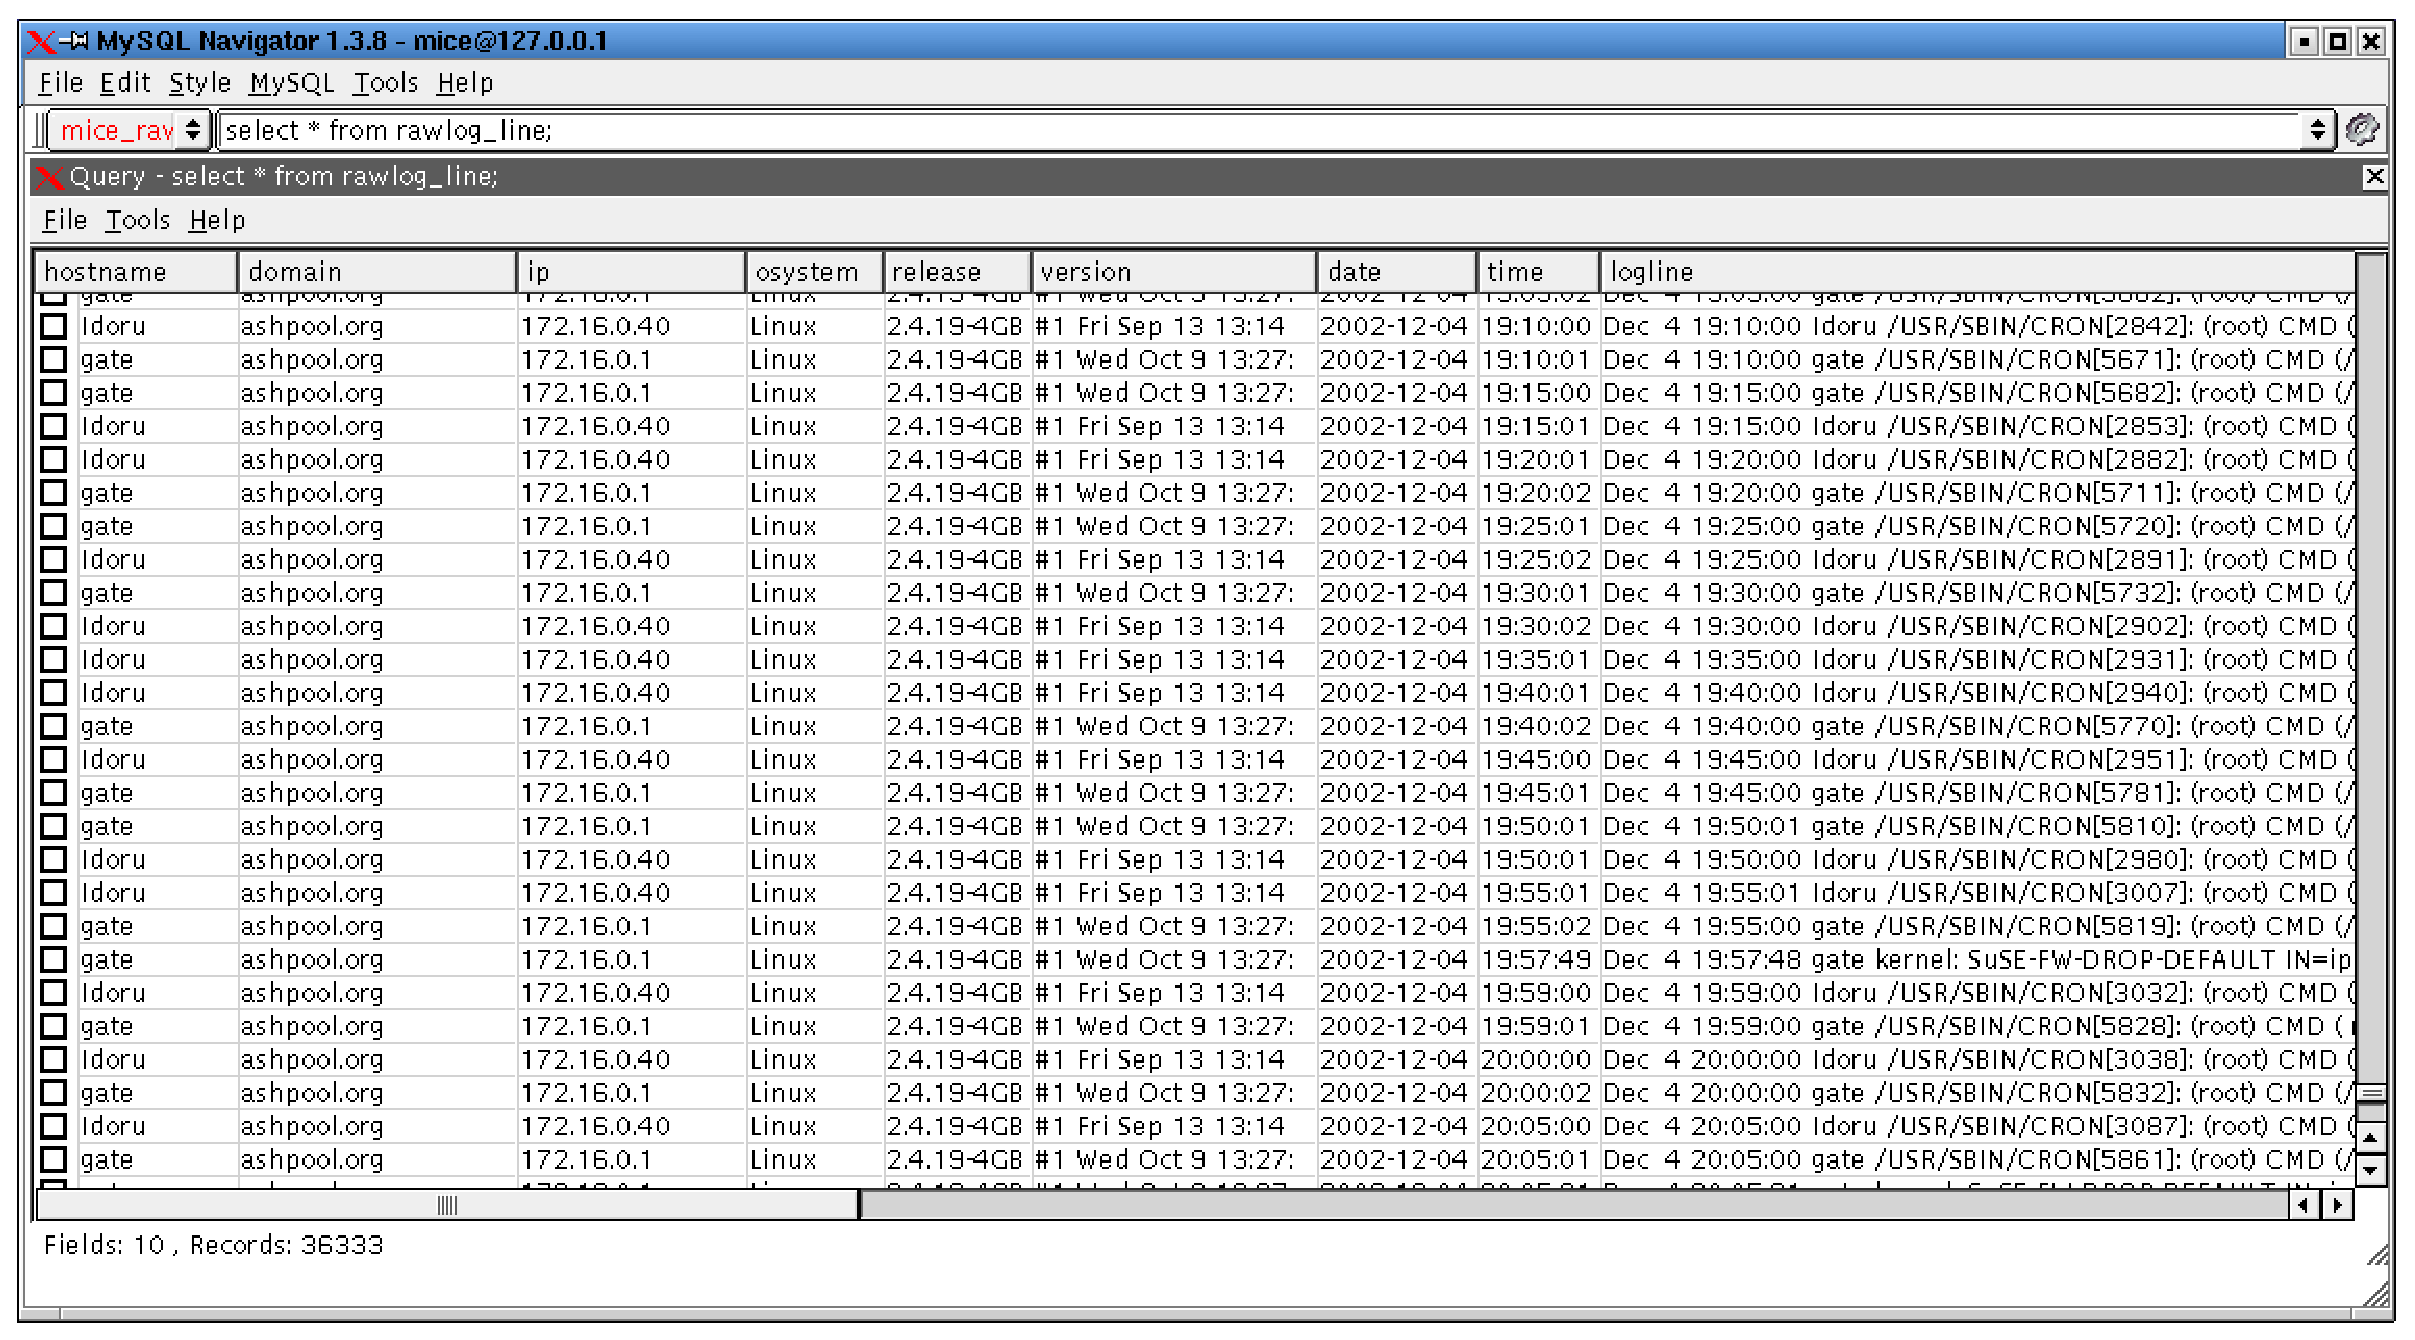
\includegraphics[scale=0.43]{snapshot-mysql-rawlog_02.eps}
	\captionof{figure}[Komplettes Auslesen der \textsf{rawlog\_line}--Tabelle]{Komplettes Auslesen der \textsf{rawlog\_line}--Tabelle}
	\vspace{0.7cm}
	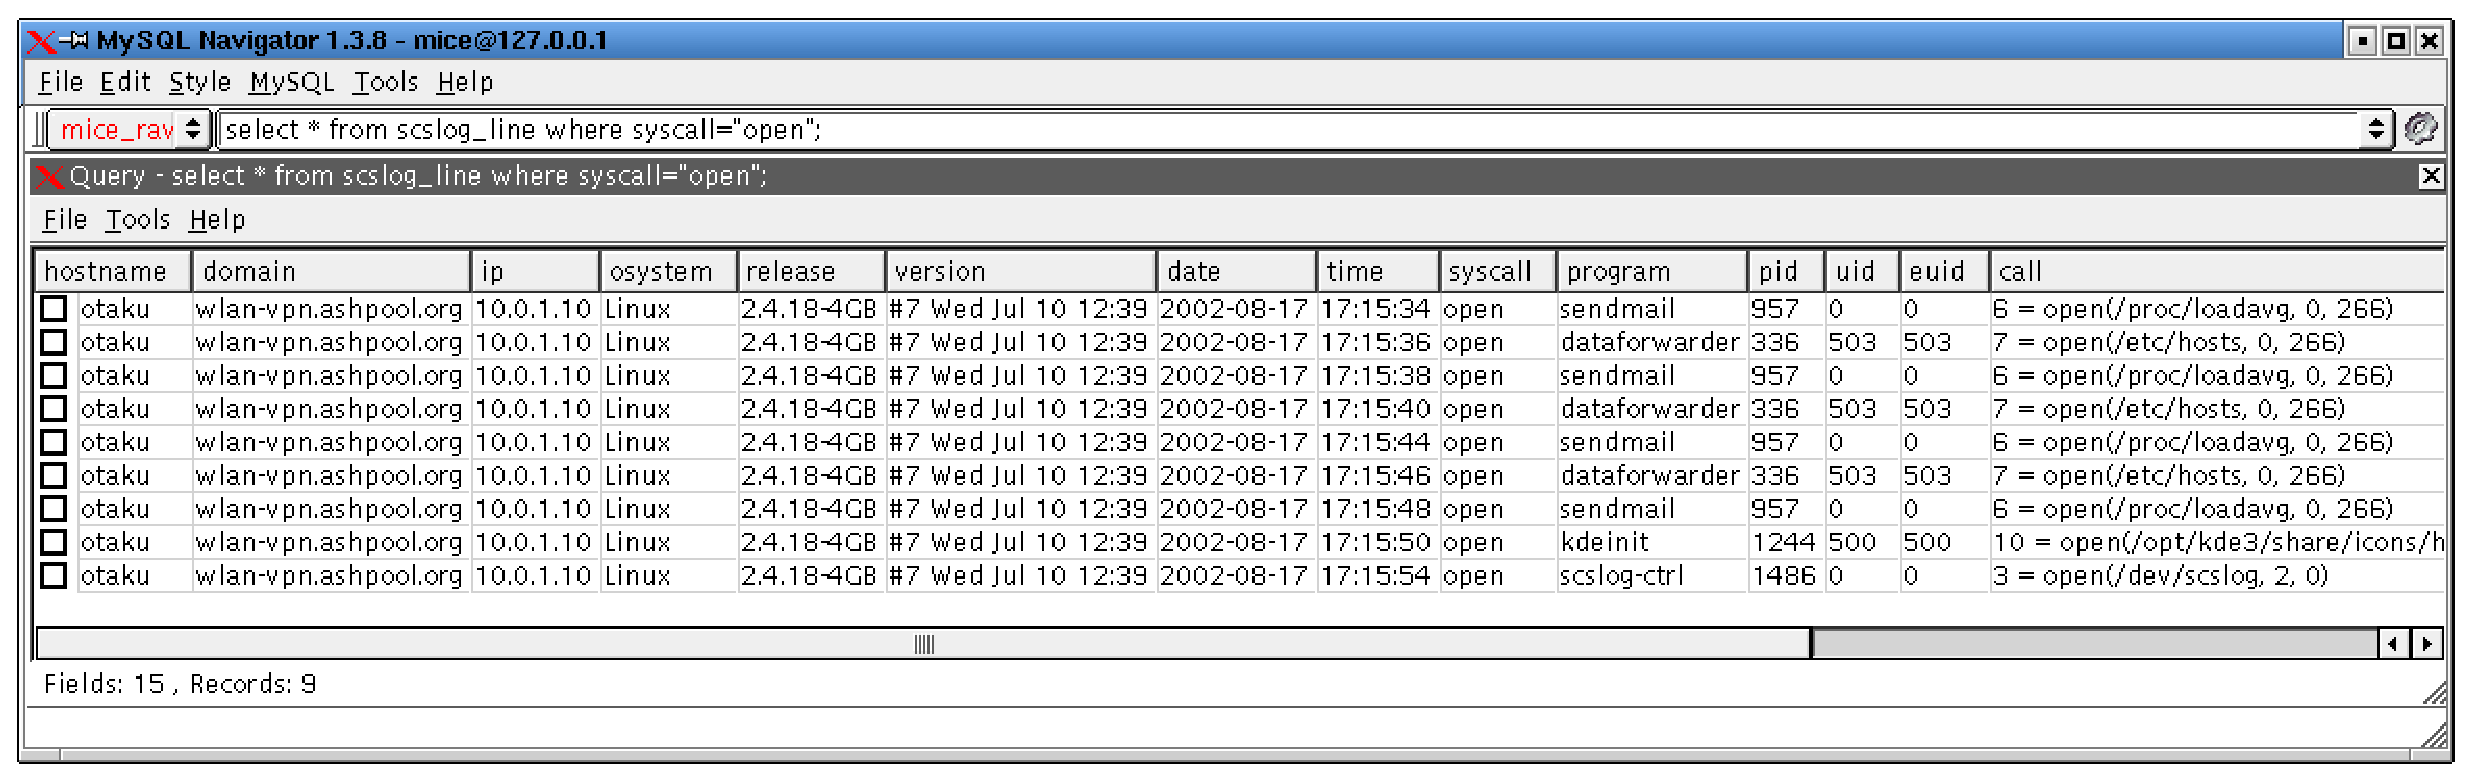
\includegraphics[scale=0.42]{snapshot-mysql-scslog_02.eps}
	\captionof{figure}[Auslesen der \textsf{scslog\_line\/}--Tabelle f"ur Syscall \texttt{open(2)}]{Auslesen der \textsf{scslog\_line\/}--Tabelle f"ur Syscall \texttt{open(2)}}
	\vspace{0.7cm}
\end{center}


\subsection{Analyseeinheit}
Das zweite Ziel der Audit--Daten ist die Analyseeinheit. Die Analyseeinheit ist "ahnlich
aufgebaut wie die Datenbank f"ur die rohen Logs, lediglich das \textit{Output Modul}
f"ur die Analyse ist ein anderes.

\pagebreak

Folgende Dateien und Verzeichnisse werden angelegt:
\begin{itemize}
	\item /var/run/M--ICE
	\item /var/log/M--ICE
	\item /lib/M--ICE
	\item /etc/M--ICE
	\item /usr/local/sbin/bufferdaemon
	\item /etc/M--ICE/bufferdaemon--aa.conf
	\item /sbin/rcMICE--bufferdaemon--aa
	\item /lib/M--ICE/mice\_mod\_aa\_regex.*
	\item /lib/M--ICE/mice\_mod\_enc\_logformat\_twofish.*
\end{itemize}

\subsubsection{Analysemodul}
Das \textit{Output Modul}  \textsf{mice\_mod\_aa\_regex} benutzt regul"are Ausdr"ucke, um die rohen
Log--Daten, die vom Client generiert wurden, nach Angriffsmustern zu durchsuchen.
Die Datei \textsf{match\_file\_aa\_regex.txt} ist Teil des Modul \textsf{mice\_mod\_aa\_regex}
und muss sp"ater auf dem Management--Host in das Verzeichnis \textsf{/etc/M--ICE/matchfiles/}
kopiert werden. Sie dient dazu, einer \textsf{AlertID} eine Beschreibung zuzuordnen.
\begin{verbatim}
[ALERT_ID]
AID = 0x1010    # RT_AUTH_S
AID = 0x1020    # RT_AUTH_F
AID = 0x2010    # RT_ROOT_W
AID = 0x2020    # RT_ROOT_O
AID = 0x2030    # RT_ROOT_R
AID = 0x2040    # RT_ROOT_S
AID = 0x2050    # RT_ROOT_E
AID = 0x3010    # RT_READ_S
AID = 0x3020    # RT_READ_F
AID = 0x4010    # RT_WRITE_S
AID = 0x4020    # RT_WRITE_F
AID = 0x5010    # RT_MONI_U
AID = 0x5020    # RT_MONI_G
AID = 0x6010    # RT_APPS_N
AID = 0x7010    # RT_EXPL
AID = 0x8010    # RT_FW_D
AID = 0x8020    # RT_FW_R
AID = 0x8030    # RT_FW_A
AID = 0x8040    # RT_FW_I


[ALERT_ID_DESCRIPTION]
AID_DESC = "Authentication Success"
AID_DESC = "Authentication Failure"
AID_DESC = "Superuser writes to File"
AID_DESC = "Superuser opens File"
AID_DESC = "Superuser reads from File"
AID_DESC = "Superuser does Operation on Socket"
AID_DESC = "Superuser executes Code"
AID_DESC = "Read Success"
AID_DESC = "Read Failure"
AID_DESC = "Write Success"
AID_DESC = "Write Failure"
AID_DESC = "Monitoring UserID"
AID_DESC = "Monitoring GroupID"
AID_DESC = "Monitoring Application"
AID_DESC = "Exploit Signature detected"
AID_DESC = "Firewall Rule: Drop"
AID_DESC = "Firewall Rule: Reject"
AID_DESC = "Firewall Rule: Accept"
AID_DESC = "Firewall Rule: Illegal"
\end{verbatim}

\vspace{1cm}

Die \textsf{AlertID} wird in der IDMEF--Nachricht in der Klasse \texttt{Classification\/} des
Elements \texttt{name\/} kodiert und wird vom Management--Host ausgewertet.
Desweiteren muss angegeben werden, welche Reaktion bei welcher \textsf{AlertID} ausgef"uhrt
wird.
\begin{verbatim}
# Write to Syslog
[RID_1]
AID_1 = 0x1010
AID_1 = 0x1020
AID_1 = 0x2010

# Send to Alert DB
[RID_2]
AID_2 = 0x5010
AID_2 = 0x5020
AID_2 = 0x6010
AID_2 = 0x7010
AID_2 = 0x8010
AID_2 = 0x8020
AID_2 = 0x8030
AID_2 = 0x8040

# Save to File
[RID_3]
AID_3 = 0x1010
AID_3 = 0x1020
AID_3 = 0x4020
AID_3 = 0x5010

# Countermeasure
[RID_4]
AID_4 = 0x6010
AID_4 = 0x7010

# EMPTY
[RID_5]
[RID_6]
[RID_7]
[RID_8]
[RID_9]
[RID_10]
\end{verbatim}

\vspace{0.5cm}

Die \textsf{Reaction ID} bezieht sich direkt auf den \textit{Reaction Process} \texttt{rid\_<nummer>\_<name>}.
In dieser Zuordnung gibt man f"ur eine Reaktion alle \textsf{AlertIDs\/} an, auf die reagiert werden soll.
Beispielsweise wird die \textsf{Reaction ID\/} 4 (Countermeasure) bei \textsf{AlertID} 0x6010
(Monitoring Applications) und 0x7010 (Exploit Patterns) ausgef"uhrt.

\vspace{0.5cm}

Die Regeln f"ur die Analyse befinden sich in der Datei \textsf{mice\_mod\_aa\_regex.conf}
im Verzeichnis \textsf{/etc/M--ICE/}. Sie sind in Kategorien, wie
\texttt{Authentication Messages}, \texttt{Root Actions}, \texttt{Syscall: read},
\texttt{Syscall: write}, \texttt{Monitoring UID, GID}, \texttt{Monitoring Application}
und \texttt{Exploit Patters}, unterteilt.
\begin{verbatim}
# Authentication Messages
[AUTH]
AuSendTo  = "M"
AuS_Rule  = ".*session started for user.*"
AuF_Rule  = ".*FAILED SU.*"
AuF_Rule  = ".*Failed password.*"
AuF_Rule  = ".*Failed rsa.*"
AuF_Rule  = ".*ROOT LOGIN REFUSED FROM.*"

# root Actions
[ROOT]
RoSendTo  = "N"
RoW_Rule  = ""
RoR_Rule  = ""
RoO_Rule  = ""
RoS_Rule  = ""
RoE_Rule  = ""

# read(2)
[READ]
ReSendTo  = "N"
ReS_Rule  = ""
ReF_Rule  = ""

# write(2)
[WRITE]
WrSendTo  = "N"
WrS_Rule  = ""
WrF_Rule  = ""

# Monitor special UID/GID
[MONITORING]
MoSendTo  = "N"
Mo_UID    = ""
Mo_GID    = ""

# Special Applications
[APPS]
ApSendTo  = "M"
Ap_Name   = ".*sshd.*"

# Exploit Patterns
[EXPLOIT]
ExSendTo = "M"
Ex_Rule = ".*crc32 compensation attack: network attack detected.*"
Ex_Rule = ".*GET /scripts/root.exe?/c+dir.*"
Ex_Rule = ".*RECV: 163129 bytes of data, 0 total lines.*"
Ex_Rule = ".*REMOTE TSI ?%.*"

# Firewall Patterns
[FIREWALL]
FwSendTo = "M"
FwD_Rule = ".*SuSE-FW-DROP.*"
FwR_Rule = ""
FwA_Rule = ".*SuSE-FW-ACCEPT.*"
FwI_Rule = ".*SuSE-FW-ILLEGAL.*"
\end{verbatim}

\subsection{Management--Host}
Der Management--Host wird ebenfalls mit Hilfe des \textit{BufferDaemons} implementiert.
Hier dient nun aber das Modul \textsf{mice\_mod\_enc\_idmef\_twofish} als \textit{Encoding Modul\/}
und \textsf{mice\_mod\_act\_generic} als \textit{Output Modul\/}.

Folgende Dateien und Verzeichnisse werden angelegt:
\begin{itemize}
	\item /var/run/M--ICE
	\item /var/log/M--ICE
	\item /lib/M--ICE
	\item /etc/M--ICE
	\item /usr/local/sbin/bufferdaemon
	\item /etc/M--ICE/bufferdaemon--mngmthost.conf
	\item /sbin/rcMICE--bufferdaemon--mngmthost
	\item /lib/M--ICE/mice\_mod\_aa\_regex.*
	\item /lib/M--ICE/mice\_mod\_enc\_idmef\_twofish.*
	\item /etc/M--ICE/rid\_1\_write\_to\_syslog.conf
	\item /usr/local/sbin/rid\_1\_write\_to\_syslog
	\item /sbin/rcMICE--rid\_1\_write\_to\_syslog
	\item /etc/M--ICE/rid\_2\_send\_to\_alert\_db.conf
	\item /usr/local/sbin/rid\_2\_send\_to\_alert\_db
	\item /sbin/rcMICE--rid\_2\_send\_to\_alert\_db
	\item /etc/M--ICE/rid\_3\_save\_to\_file.conf
	\item /usr/local/sbin/rid\_3\_save\_to\_file
	\item /sbin/rcMICE--rid\_3\_save\_to\_file
	\item /etc/M--ICE/rid\_4\_countermeasure.conf
	\item /usr/local/sbin/rid\_4\_countermeasure
	\item /sbin/rcMICE--rid\_4\_countermeasure
\end{itemize}

\vspace{1cm}
\begin{center}
	\includegraphics[scale=0.5]{MH-Datenfluss.eps}
	\captionof{figure}{Datenflussdiagramm des Management--Hosts}
\end{center}
\vspace{1cm}


\subsubsection{Act--Generic Modul}
Bei der Entwicklung dieses Moduls wurde darauf geachtet, dass es nicht nur auf IDMEF--Alarme
des RegEx--Modul reagieren kann, sondern auch auf Analyseeinheiten anderer Systeme.
Diese Funktionalit"at wird durch die sog. \textit{Match Files\/} erreicht.
Die \textsf{Analyzer ID\/}, die in der IDMEF--Nachricht kodiert ist, wird dazu benutzt,
das richtige \textit{Match File\/} ausfindig zu machen. Die Zuordnung findet in der
Konfigurationsdatei von \textsf{mice\_mod\_act\_generic.conf} statt.
\begin{verbatim}
# Every Analyzer must send an ID...
[ANALYZER_ID]
ANAID = "MICE-RegEx"

# ... to select the right file for matching Alert ID -> Reaction ID
[ANALYZER_MATCHFILE]
MF = match_file_aa_regex.txt
\end{verbatim}

\vspace{0.5cm}

In der selben Datei wird auch der Zusammenhang von \textsf{Reaction ID} und FIFO
hergestellt. An jedem FIFO lauscht ein \textit{Reaction Process\/}. Zur besseren
"Ubersicht tr"agt der FIFO den selben Namen wie der \textit{Reaction Process\/}.
\begin{verbatim}
# List of Reaction IDs
[REACTION_ID]
RID = 1
RID = 2
RID = 3
RID = 4

# and associated named pipes
[RID_PIPENAME]
PIPE = rid_1_write_to_syslog
PIPE = rid_2_send_to_alert_db
PIPE = rid_3_save_to_file
PIPE = rid_4_countermeasure
\end{verbatim}


\subsubsection{Reaktionsprozesse}
Durch die flexible Architektur des Management--Hosts l"asst sich jeder denkbare
\textit{Reaction Process\/} implementieren. Starten "uber rc--Skript:
\begin{verbatim}
root@management host# rcMICE-rid_1_write_to_syslog start
M-ICE IDS: Starting Reaction Service 'rid_1_write_to_syslog'         done
root@management host# rcMICE-rid_2_send_to_alert_db start
M-ICE IDS: Starting Reaction Service 'rid_2_send_to_alert_db'        done
root@management host# rcMICE-rid_3_save_to_file start
M-ICE IDS: Starting Reaction Service 'rid_3_save_to_file'            done
root@management host# rcMICE-rid_4_countermeasure start
M-ICE IDS: Starting Reaction Service 'rid_4_countermeasure'          done
\end{verbatim}

\subsubsection{Datenbank f"ur Alarme}
Die MySQL--Datenbank f"ur Alarme l"auft in unserem Fall direkt auf dem Management--Host
und wird vom \textit{Reaction Process\/} \textsf{rid\_2\_send\_to\_alert\_db} versorgt.

\subsubsection{Tabellen erstellen}
Diese Tabelle enth"alt alle n"otigen Informationen aus der IDMEF--Nachricht.
Um die Tabelle zu erstellen sind folgende Schritte n"otig:
\begin{itemize}
	\item Erstellen der Datenbank \textsf{alert\_db}
	\item Tabellen generieren mit \texttt{mysql mice\_rawlog\_tab $<$ create\_mysql\_tab\_for\_alert\_logs.txt}
	\item User \texttt{alertdb} einrichten
	\item INSERT-- sowie SELECT--Operation f"ur den Benutzer auf Datenbank \textsf{alert\_db} erlauben
\end{itemize}

\subsubsection{Tabellen auslesen}
Die Alarm--Datenbank kann nun mit einem MySQL Client ausgelesen werden.

\begin{center}
	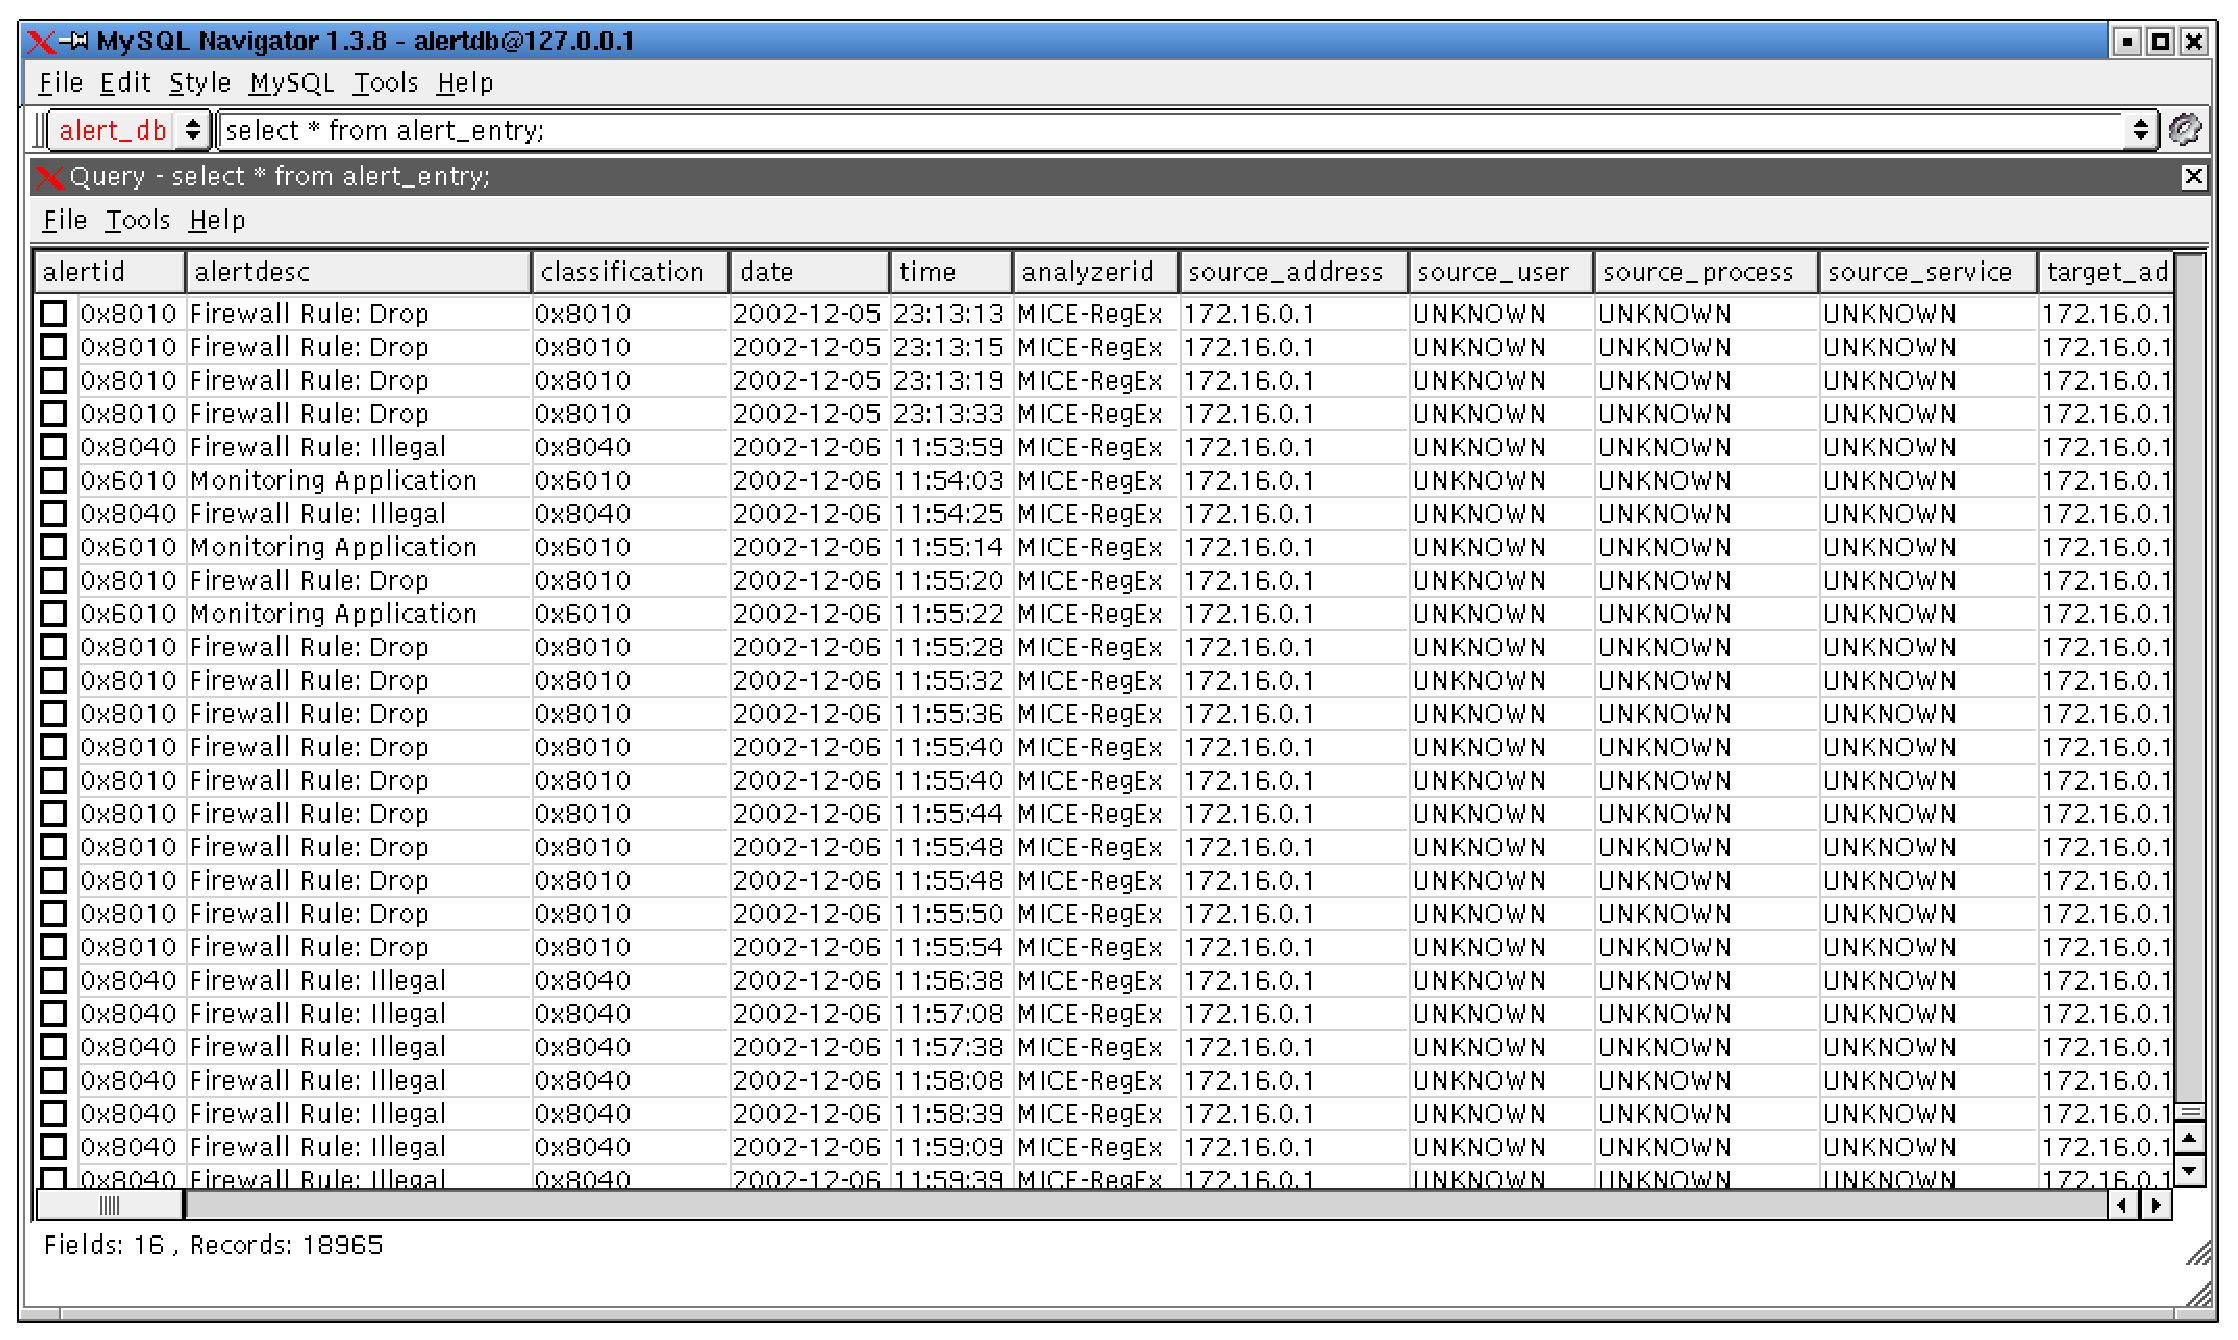
\includegraphics[scale=0.42]{snapshot-mysql-alertdb_04.eps}
	\captionof{figure}{Komplettes Auslesen der \textsf{alert\_entry} Tabelle}
	\vspace{0.7cm}
	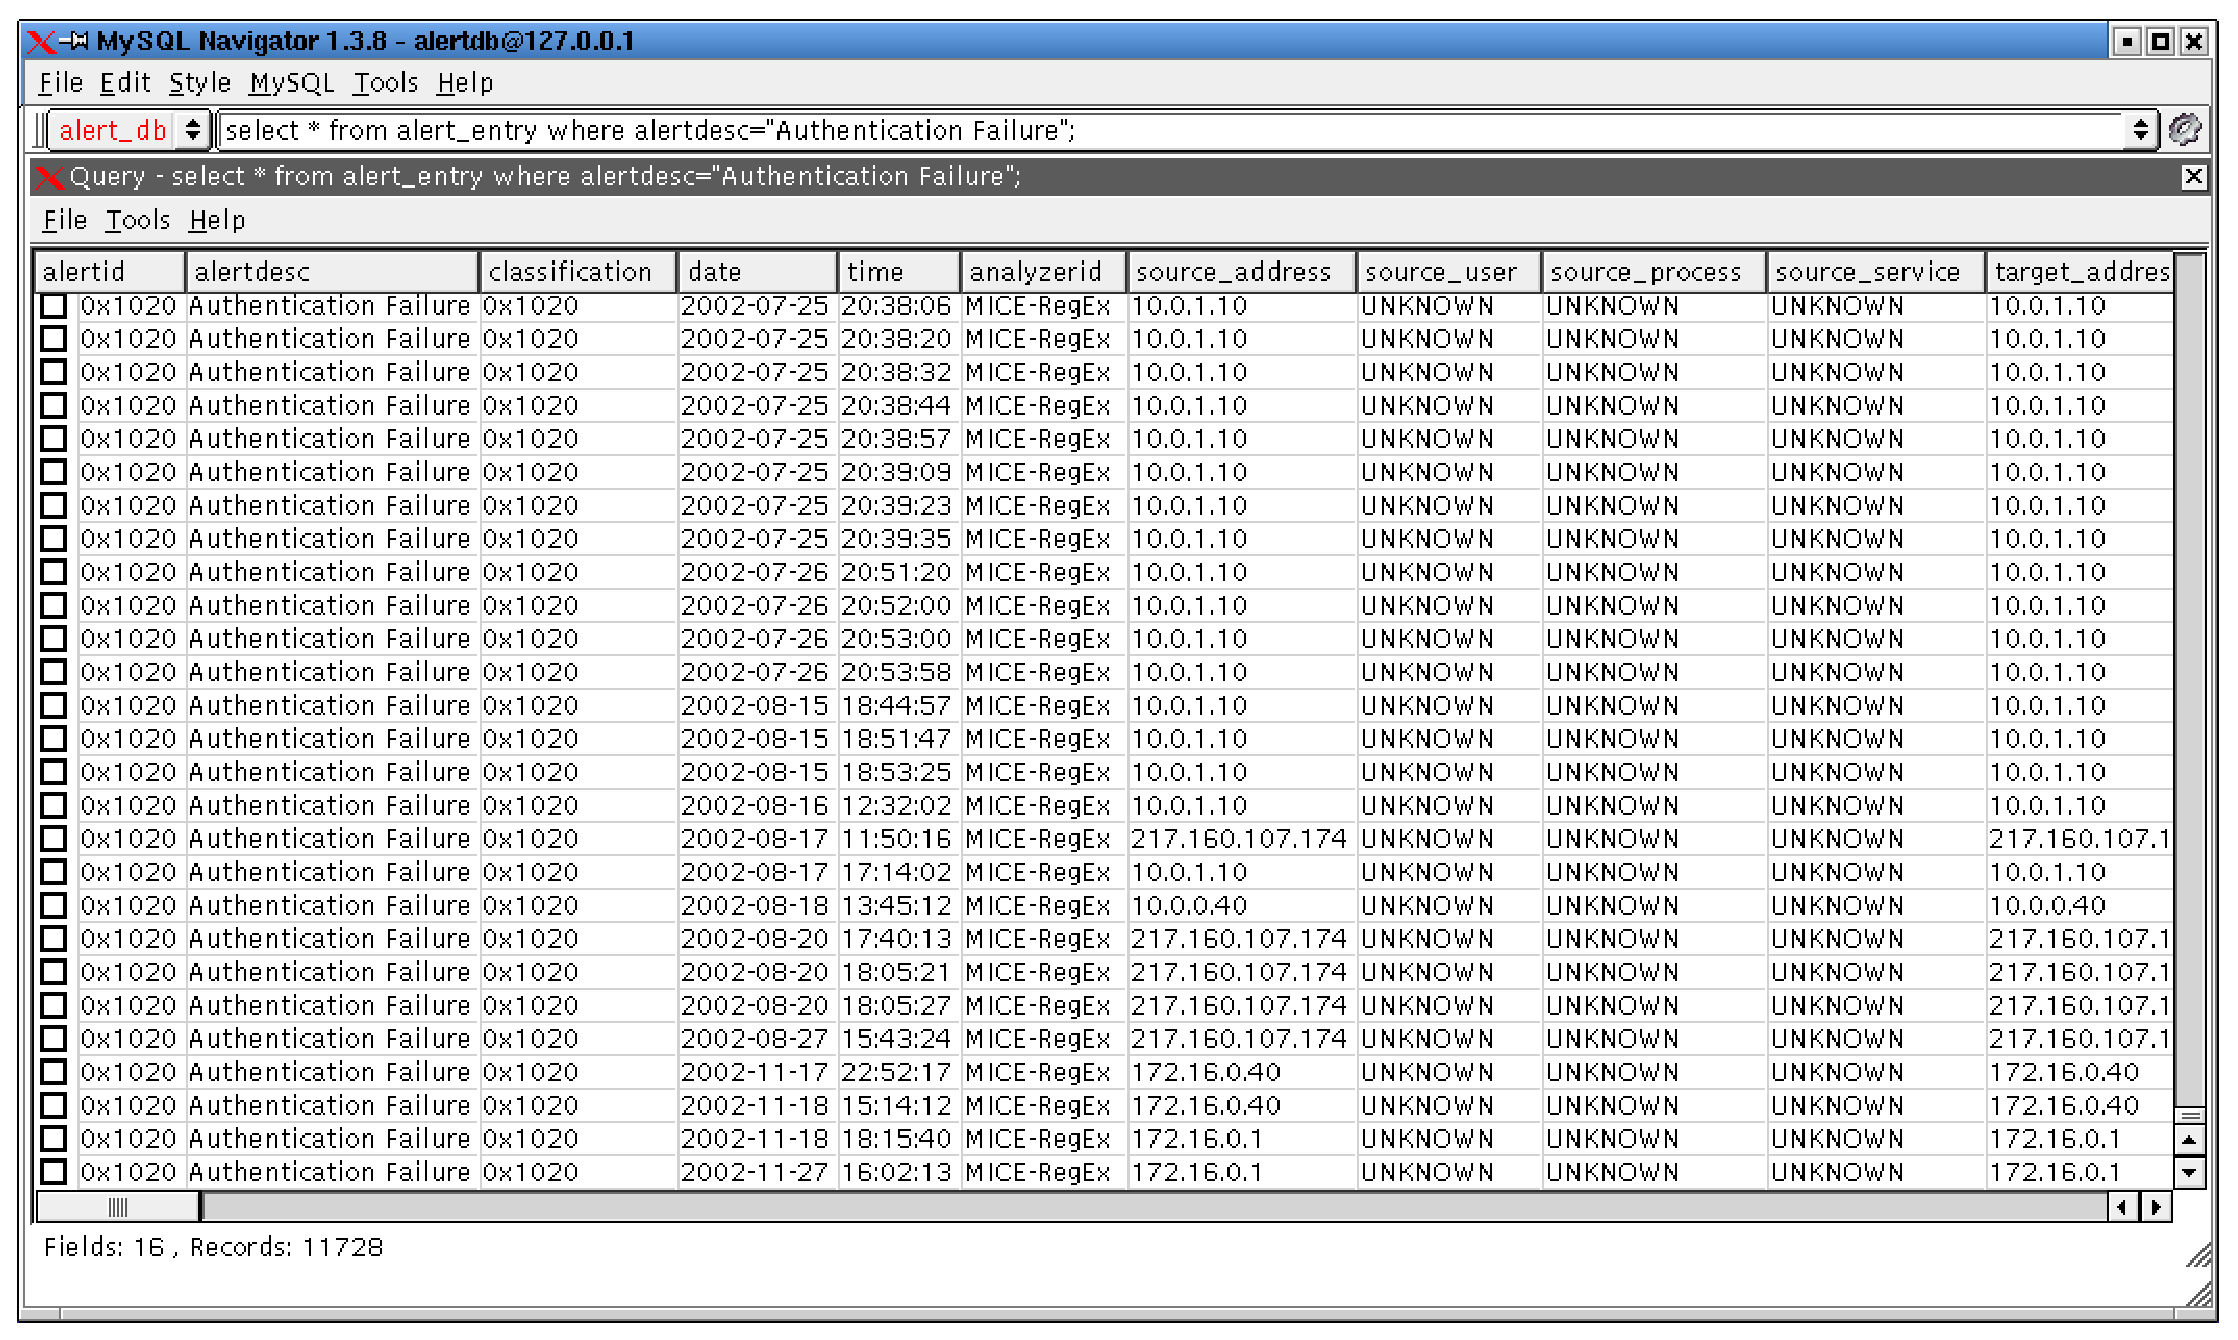
\includegraphics[scale=0.42]{snapshot-mysql-alertdb_05.eps}
	\captionof{figure}{Auslesen der \textsf{alert\_entry} Tabelle f"ur alle fehlgeschlagenen Authentifizierungen}
\end{center}



%
%% Kapitel
%
\chapter{Testergebnisse}
\textsc{M--ICE} wurde einigen Tests unterzogen, bei denen mehr auf Fehlerbehebung als auf Performanz
R"ucksicht genommen wurde. Der Grund daf"ur, ist die Tatsache, dass der Flaschenhals eines solchen
Systems beim Datentransport und bei der Datenanalyse liegt.
Der Datentransport lie"se sich neben breitbandigen Netzen und schnelleren Computersystemen, vor allem durch
bessere Aufteilung der IDS--Komponenten beschleunigen. Zudem ist die Datenanalyse, ausser zu Testzwecken,
nicht Bestandteil der Entwicklung gewesen; ein Test w"urde also keinen Sinn machen. Trotzdem sind nat"urlich
einige Ergebnisse zu Tage getreten.

Als Testumgebung diente folgender Aufbau.
\vspace{1cm}
\begin{center}
	\includegraphics[scale=0.26]{Testnetzwerk_02.eps}
	\captionof{figure}{Aufbau des Testnetzwerkes}
\end{center}
\vspace{1cm}

Bei dieser Testumgebung lief die Analyseeinheit, die Datenbanken und der Management--Host auf dem Rechner
\textsc{Wintermute}. Als Client dienten f"unf Rechner (\textsc{Idoru}, \textsc{Otaku}, \textsc{HakNam},
\textsc{Gate}, \textsc{www.uin4d.de}) in verschiedenen Netzwerken.
Folgende Tabelle zeigt die Hardware-- und Softwareausstattung der einzelnen Rechner:
\begin{center}
	\begin{tabular}{|c|c|c|c|c|}
		\hline
		\textbf{Name}		& \textbf{CPU}	& \textbf{RAM}	& \textbf{Netzanbindung}	& \textbf{Betriebssystem}	\\ \hline
		\textsc{Wintermute}	& 2 x 700 MHz	& 1 GB		& 100 Mbit (Intranet)		& SuSE Linux 8.0		\\ \hline
		\textsc{Idoru}		& 733 MHz	& 128 MB	& 100 Mbit (Intranet)		& SuSE Linux 8.0		\\ \hline
		\textsc{Otaku}		& 700 MHz	& 256 MB	& $<=$ 10 Mbit (WLAN)		& SuSE Linux 8.0		\\ \hline
		\textsc{HakNam}		& 266 MHz	& 128 MB	& 10 Mbit (DMZ)			& SuSE Linux 7.0		\\ \hline
		\textsc{Gate} (Router)	& 266 MHz	& 128 MB	& 10/100 Mbit / 64 Kbit 	& SuSE Linux 8.1		\\ \hline
		\textsc{www.uin4d.de}	& 1,2 GHz	& 256 MB	& 64 Kbit (Internet)		& SuSE Linux 7.2		\\ \hline
	\end{tabular}
\end{center}
\vspace{1cm}

Die meisten Daten werden vom \textit{DataForwarder\/} generiert, da er den Datenstrom dupliziert und
u.U. noch ins gleiche Netzsegment sendet. Um hier einen m"oglichen Engpass zu vermeiden, k"onnte man den
\textit{DataForwarder\/} so einrichten, dass er die Audit--Daten nur an die Datenbank sendet,
aber nicht an die Analyseeinheit. Das \textit{Encoding Modul\/} des Analysesystems m"usste sich nun
in gewissen Zeitintervallen die Audit--Daten von der Datenbank holen. Somit gehen die Daten zwar immernoch
zweimal "uber das Netzwerk, jedoch nicht zum selben Zeitpunkt. Desweiteren k"onnte man die Datenbank und
die Analyseeinheit auf dem selben Rechner installieren und so noch mehr Bandbreite einsparen. Ein zus"atzlicher
Vorteil f"ur die Analyse w"urde sich aus der Tatsache ergeben, dass die rohen Log--Daten bereits in
logische Teile zerlegt wurden, was die Analyse vereinfacht. Nachteil ist die Abh"angigkeit von der
Datenbank und die Aufteilung der Hardware--Ressourcen.

Gl"ucklicherweise tauchten diese theoretischen Probleme nicht in der Praxis auf. Selbst der Rechner
\textsc{www.uin4d.de}, welcher nur "uber eine ISDN--Leitung angebunden war, und auf dem ein "offentlicher
Web-- und Gameserver l"auft und durchschnittlich drei Benutzer gleichzeitig arbeiten, hat die
Bandbreite nicht saturieren k"onnen.

Die meisten Audit--Daten wurden vom Paketfilter des Routers \textsc{Gate} erzeugt. Durch die st"andigen
\textit{Scans} nach offenen SMB Ports entstanden eine Menge uninteressanter Daten. Innerhalb von 7,5 Stunden
wurden vom Paketfilter 392 Pakete abgewiesen, 332 davon waren UDP Pakete mit dem Zielport 137 (SMB).
Unser IDS ist in der Lage diese ungef"ahrlichen Angriffsversuche bereits auf dem Client auszufiltern. Dank
des Filter--Moduls im \textit{DataForwarder} und der entsprechenden Filterregel
(\texttt{.* PROTO=UDP .* DPT=137 .*}) konnte das Datenvolumen stark reduziert werden. In diesem Fall
sind es sogar ca. 80 \% weniger Daten, die gespeichert und analysiert werden m"ussen.

Die Rechner \textsc{Gate} und \textsc{Idoru} generieren innerhalb von 15 Stunden etwa 840 Eintr"age in
der \textsf{rawlog\_line}-Tabelle. Nach der Analyse befinden sich ca. 475 Eintr"age in der
\textsf{alert\_entry}--Tabelle.
Davon sind 466 Eintr"age vom Typ \texttt{Firewall Rule: Drop} und die restlichen von Typ
\texttt{Firewall Rule: Illegal}, \texttt{Authentication Success} und \texttt{Monitoring Applikation}.
Hier sieht man, wie selbst die einfache Analyse durch regul"are Ausdr"ucke, das Datenaufkommen um knapp
50 \% reduzieren kann.

Die maximale Gr"o"se eines Client--Paketes betr"agt 1710 Byte. \textsc{Gate} sendet in 15 Stunden
je 760 Pakete an die Datenbank f"ur rohe Log--Daten und an die Analyseeinheit, dass sind
weniger als 170 KByte pro Stunde. Datenmengen dieser Dimension fallen bei heutigen Vernetzungstechnologien
sogut wie gar nicht ins Gewicht. In einem 100 MBit Netzwerk, mit einer angenommenen realen
Transportgeschwindigkeit von 8 MByte/s, w"urde man ungef"ahr 170.000 Rechner, mit einem Audit--Datenvolumen,
vergleichsweise mit dem von \textsc{Gate}, ben"otigen, um das Netzwerk voll auszulasten.
Diese Zahlen machen sehr deutlich, dass der bef"urchtete Engpass nicht existiert.

Der Anstieg der Rechnerauslastung war ebenfalls kaum merkbar, selbst nicht auf \textsc{Wintermute},
der immerhin fast alle IDS--Komponenten beherbergte.

Der \textit{DataForwarder} belegte ca. 0,6 \% des Speichers auf dem Client--System \textsc{Gate}.
Dieser Wert wird haupts"achlich durch die Gr"o"se des \textit{Shared Memory Segments} bestimmt.
Zum Zeipunkt der Datenweiterleitung wurde eine Prozessorauslastung von 0,3 \% gemessen.

Im Fall der Analyseeinheit ben"otigt der \textit{BufferDaemon} im Leerlauf 0,2 \% des Speichers
und 0,0 \% der Prozessorleistung. W"ahrend der Datenanalyse stieg lediglich die Prozessorauslastung
auf 0,1 \%.


Ein weiterer wichtiger Faktor ist die Reaktionsgeschwindigkeit. Als Reaktion wird auf dem
Client (\textsc{Gate}) eine Datei im Verzeichnis \textsf{/tmp} angelegt. Um die
Geschwindigkeit der Verarbeitung bis zur Reaktion messen zu k"onnen, wurde ein kleines
Programm entwickelt, das zwei Threads startet. Ein Thread l"ost eine Aktion aus und
protokolliert die Startzeit. Die Aktion veranlasst den Management--Host (\textsc{Wintermute})
dazu, eine Reaktion auf dem Client--System auszuf"uhren. Der zweite Thread pr"uft wann die Reaktion
auftritt und misst ebenfalls die Zeit. Der Haupt--Thread berechnet dann die Differenz der beiden
Zeitwerte und gibt diese als Ergebnis aus. Es wurden mehrere Messungen durchgef"uhrt. Die
gemessende Reaktionszeit lag zwischen 51 und 71 Sekunden. Anschlie"send wurde nacheinander die
Priorit"at (\textit{Nice Value}: --10) der folgenden Prozesse erh"oht:
\begin{itemize}
	\item ReactionDaemon
	\item DataForwarder
	\item Analysis--Agent
	\item Management--Host
	\item Syslog--Daemon (Client--System)
\end{itemize}
Erstaunlicherweise brachte die Priorit"atenerh"ohung keine Beschleunigung der Reaktion.
In angesicht der Tatsache, dass das Netzwerk keinen Engpass darstellt, l"a"st das Ergebnis
nur den Schluss zu, dass die Operationen von \textsc{M--ICE} sich durch Priorit"atenerh"ohung
nicht beschleunigen lassen, oder dass die Verarbeitungszeit der \textsc{M--ICE}--Komponenten
nicht ausschlaggebend ist.


%Der einzige gro"se Performanzeinbruch wurde bei der Abfrage der Datenbanken festgestellt.
%Wenn etwa eine SQL--Anfrage abgesetzt wurde, die mehrere tausend Datenbankeintr"age zur"uckgab,
%dann stieg die Prozessorauslastung f"ur den MySQL--Server auf "uber 90 \% und das Ergebnis
%erschien erst nach einigen Minuten. Dieses Problem konnte jedoch einfach durch die Verwendung
%von Spaltenindices in der SQL--Datenbank behoben werden (\texttt{CREATE INDEX index\_name ON table column}).


%
%% Kapitel
%
\chapter{Schlussbetrachtung}
Abschlie"send kann man sagen, dass alle n"otigen Eigenschaften eines hostbasierten Intrusion--Detection
Systems implementiert werden konnten. \textsc{M--ICE} bietet die M"oglichkeit, Audit--Daten zu generieren,
zu klassifizieren, zu speichern und entsprechende Gegenreaktionen auszul"osen.
Leider konnte aufgrund von Zeitmangel die Heartbeat--Komponente und die kryptografische Signatur f"ur
die Datenbankeintr"age nicht realisiert werden.

Die vorhandene, modulare Architektur erlaubt es, mit wenig Aufwand, ein sehr leistungsf"ahiges
und professionelles IDS zu bauen. Die hier, nur zu Testzwecken, implementierte Analyseeinheit auf
Basis von regul"aren Ausdr"ucken, lie"se sich leicht durch die auf Zustandsautomaten aufbauende, freie
Analyse--Engine \textit{STAT\/} der Universit"at von Californien, Santa Barbara \cite{www-stat} ersetzen.
Zudem bietet die UCSD bereits vielf"altige Muster f"ur die Angriffserkennung an. Diese Angriffsmuster nutzen
bspw. das \textit{Common Logging Format\/} des Apache Webserver oder den Log--Output von Solaris'
\textit{Basic Security Module\/} (BSM). F"ur letzteres Format gibt es eine, leider nicht mehr
weiterentwickelte, Implementierung f"ur Linux, so dass man die BSM--Angriffsmuster f"ur \textit{SCSLog}
umschreiben m"usste.

\textsc{M--ICE} soll in Zukunft weiterentwickelt werden, da es in der Testphase vielversprechende
Ergebnisse geliefert hat und die Entwicklung sehr lehrreich war.


% leere Seite
\clearpage
\mbox {~}
\clearpage

%%
%% Anhang
%%

\appendix
%\begin{appendix}

%
%%
%
\chapter{Terminologie und Abk"urzungen}
\begin{itemize}
	\item[\textbf{BSM}]		Basic Security Module
	\item[\textbf{CERT}]		Computer Emergency Response Team
	\item[\textbf{DMZ}]		Demilitarisierte Zone, bspw. sicheres Netz zw. Internet und internem Netz
	\item[\textbf{DoS}]		Denial--of--Service
%	\item[\textbf{False Negative}]	Nicht erkannter Angriff
%	\item[\textbf{False Positive}]	Inkorrekt erkannter Angriff
	\item[\textbf{FIFO}]		First In, First Out; Named Pipe; lokale Interprozesskommunikation
	\item[\textbf{GNU}]		GNU's Not Unix!, Projekt der \textit{Free Software Foundation\/} zur Entwicklung von freien Unix--Tools
	\item[\textbf{GUI}]		Graphical User Interface
	\item[\textbf{IAP}]		Intrusion Alert Protocol
	\item[\textbf{IDXP}]		Intrusion Detection Exchange Format
	\item[\textbf{IDMEF}]		Intrusion Detection Message Exchange Format
	\item[\textbf{IDS}]		Instrusion Detection System
	\item[\textbf{IP}]		Internet Protocol, s. RFC--791 \cite{www-rfcdb}
	\item[\textbf{LKM}]		Loadable Kernel Modul
	\item[\textbf{M--ICE}]		Modular Intrusion Detection and Countermeasure Environment
	\item[\textbf{NTP}]		Network Time Protocol, s. RFC--1119 \cite{www-rfcdb}
	\item[\textbf{PGP}]		Pretty Good Privacy, eMail Verschl"usselungsprogramm
	\item[\textbf{PKI}]		Public Key Infrastructure
	\item[\textbf{RegEx}]		Regular Expressions, regul"are Ausdr"ucke
	\item[\textbf{RPC}]		Remote Procedure Call
	\item[\textbf{SMB}]		Server Message Block
	\item[\textbf{SNMP}]		Simple Network Management Protocol
	\item[\textbf{SO}]		Security Officer
	\item[\textbf{SQL}]		Structured Query Language
	\item[\textbf{SSL}]		Secure Socket Layer, Verschl"usselung auf Pr"asentationsebene
	\item[\textbf{Syslog}]		natives Unix Logsystem
	\item[\textbf{TCP}]		Transmission Control Protocol, s. RFC--793 \cite{www-rfcdb}
	\item[\textbf{UDP}]		User Datagram Protocol, s. RFC--768 \cite{www-rfcdb}
	\item[\textbf{UML}]		Unified Modeling Language
	\item[\textbf{VPN}]		Virtual Private Network
	\item[\textbf{VM}]		Virtual Machine
	\item[\textbf{XML}]		Extensible Markup Language
\end{itemize}

%
%% Abbildungsverzeichnis
%

\listoffigures

%
%% Literaturverweise
%

%\thispagestyle{empty}

\begin{thebibliography}{100}
\bibitem[1] {draft-idmef}		D. Curry, H. Debar, Intrusion Detection Message Exchange Format --- Data Model and Extensible Markup Language (XML) Document Type Definition, IDWG, February 2002
\bibitem[2] {draft-iap}			Gupta, Buchheim, Feinstein, Harvey Mudd College, Matthews, Pollock, IAP: Intrusion Alert Protocol, IDWG, March 2001
\bibitem[3] {draft-idxp}		Feinstein, Matthews, White, Harvey Mudd College, MITRE Corporation, The Intrusion Detection Exchange Protocol (IDXP), IDWG, May 2001
\bibitem[4] {paper-syscall-seq}		Hofmeyr, Forrest, Somayaji, Intrusion Detetction using Sequences of System Calls, August 1998
\bibitem[5] {paper-pseudo-1}		Biskup, Flegel, On Pseudoymization of Audit Data for Intrusion--Detection, July 2000
\bibitem[6] {paper-pseudo-2}		Sobirey, Fischer--H"ubner, Rannenberg, Pseudonymous Audit for Privacy Enhanced Intrusion--Detection, 1997
\bibitem[7] {paper-pseudo-3}		Flegel, Pseudonymizing Unix Log Files
\bibitem[8] {paper-anforderungen}	von Helden, Grundlagen, Forderungen und Markt"ubersicht f"ur Intrusion Detection Systeme (IDS) und Intrusion Response Systeme (IRS), debis IT Security Service, Studie f"ur das \textit{Bundesamt f"ur Sicherheit in der Informationtechnik\/} (BSI), 1998
\bibitem[9] {book-bace-id}		Rebecca Gurley Bace, Intrusion--Detection, MTP, 2000
\bibitem[10]{book-proctor-id-handbook}	Paul E. Proctor, The Practical Intrusion Detection Handbook, Prentice Hall, 2001
\bibitem[11]{book-crypto-1}		Bruce Schneier, Angewandte Kryptographie, Addison--Wesley, 1996
\bibitem[12]{www-cert-stats}		CERT Statistiken: \url{http://www.cert.org/stats/cert_stats.html}
\bibitem[13]{www-cidf}			Common Intrusion Detection Framework (CIDF), \url{http://www.gidos.org}
\bibitem[14]{paper-bishop}		Matt Bishop, Standard Audit Trail Format, 1995 National Information Systems Security Conference, pages 136--145
\bibitem[15]{paper-cisl}		Common Intrusion Specification Language (CISL), \url{http://www.gidos.org/drafts/language.txt}
\bibitem[16]{www-nids}			Next Generation IDS (NIDS), \url{http://www.sdl.sri.com/nides/index.html}
\bibitem[17]{www-aid}			AID, \url{http://www-rnks.informatik.tu-cottbus.de/de/security/aid.html}
\bibitem[18]{www-specter}		Specter, \url{http://www.specter.ch/}
\bibitem[19]{www-snort}			Snort, \url{http://www.snort.org}
\bibitem[20]{www-packetmonster}		Packet Monster, \url{http://www.inas.mag.keio.ac.jp/ids/pakemon/}
\bibitem[21]{www-prelude}		Prelude, \url{http://prelude-ids.org/}
\bibitem[22]{www-dtk}			Deception ToolKit, \url{http://www.all.net/dtk/}
\bibitem[23]{www-aafid}			Autonomous Agents for Intrusion Detection (AAFID), \url{http://www.cerias.purdue.edu/coast/projects/aafid.html}
\bibitem[24]{www-emerald}		Emerald, \url{http://www.sdl.sri.com/emerald/}
\bibitem[25]{www-honeynet}		The Honeynets Project, \url{http://project.honeynet.org}
\bibitem[26]{www-clips}			CLIPS, \url{http://www.unet.univie.ac.at/~a9715573/res/clips.html}
\bibitem[27]{www-psionic}		Psionic Software, \url{http://www.psionic.com/}
\bibitem[28]{www-idwg}			IDWG, \url{http://www.silicondefense.com/idwg/}
\bibitem[29]{paper-evasion}		Thomas H. Ptacek und Timothy N. Newsham, Inseration, Evasion and Denial of Service: Eluding Newtork Intrusion--Detection,\url{http://www.robertgraham.com/mirror/Ptacek-Newsham-Evasion-98.html}
\bibitem[30]{www-kerberos}		MIT Kerberos, \url{http://web.mit.edu/kerberos/www/}
\bibitem[31]{www-needham}		RM Needham, MD Schrieder, \grqq Using Encryption for Authentication in Large Networks of Computers\grqq, in \textit{Communications of the ACM}, v21 no 12 (Dec 1978), pp 993--999
\bibitem[32]{www-libtool}		Libtool, \url{http://www.gnu.org/software/libtool/}
\bibitem[33]{www-libidmef}		LibIDMEF, \url{http://www.silicondefense.com/idwg/libidmef/index.htm}
\bibitem[34]{www-stat}		    	STAT, \url{http://www.cs.ucsb.edu/~rsg/STAT/}
\bibitem[35]{www-libiap}	    	LibIAP, \url{http://snortnet.scorpions.net/}
\bibitem[36]{www-libmcrypt}		LibMCrypt, \url{http://mcrypt.hellug.gr}
\bibitem[37]{www-rfcdb}			RFC Datenbank, \url{http://www.rfc-editor.org/}
\bibitem[38]{www-rsasec}		RSA Security, \url{http://www.rsasecurity.com/}
\bibitem[39]{www-libidxp}		LibIDXP, \url{http://idxp.codefactory.se/}
\end{thebibliography}


% leere Seite
\clearpage
\mbox {~}
\clearpage


%
%% �26(1) DPO
%
\chapter{Erkl"arung gem"a"s \S26 (1) DPO}
Hiermit erkl"are ich, dass die Diplomarbeit von mir selbstst"andig verfasst und angefertigt
wurde, nur die angegebenen Quellen und Hilfsmittel benutzt wurden und Zitate kenntlich gemacht
wurden.

\vspace{3cm}

\hspace{9cm} -------------------------------------- \\
\vspace{2mm}
\hspace{10cm} \small{Unterschrift (Thomas Biege)}

%\end{appendix}

\end{document}
